\documentclass[journal]{IEEEtran}
\usepackage[a5paper, margin=10mm]{geometry}
%\usepackage{lmodern} % Ensure lmodern is loaded for pdflatex
\usepackage{tfrupee} % Include tfrupee package


\setlength{\headheight}{1cm} % Set the height of the header box
\setlength{\headsep}{0mm}     % Set the distance between the header box and the top of the text


%\usepackage[a5paper, top=10mm, bottom=10mm, left=10mm, right=10mm]{geometry}

%
\usepackage{gvv-book}
\usepackage{gvv}
%\setlength{\intextsep}{10pt} % Space between text and floats

\makeindex

\begin{document}
\bibliographystyle{IEEEtran}
\onecolumn


\title{
	%\begin{flushleft}
	\begin{center}
	%MATRICES \\ In Geometry
	Algebra
%	Progressions
	\\
\rule{0.4\columnwidth}{0.4pt}
%\end{flushleft}
\end{center}
}
\author{
\vspace{11cm}
	%\begin{flushleft}
	\begin{center}
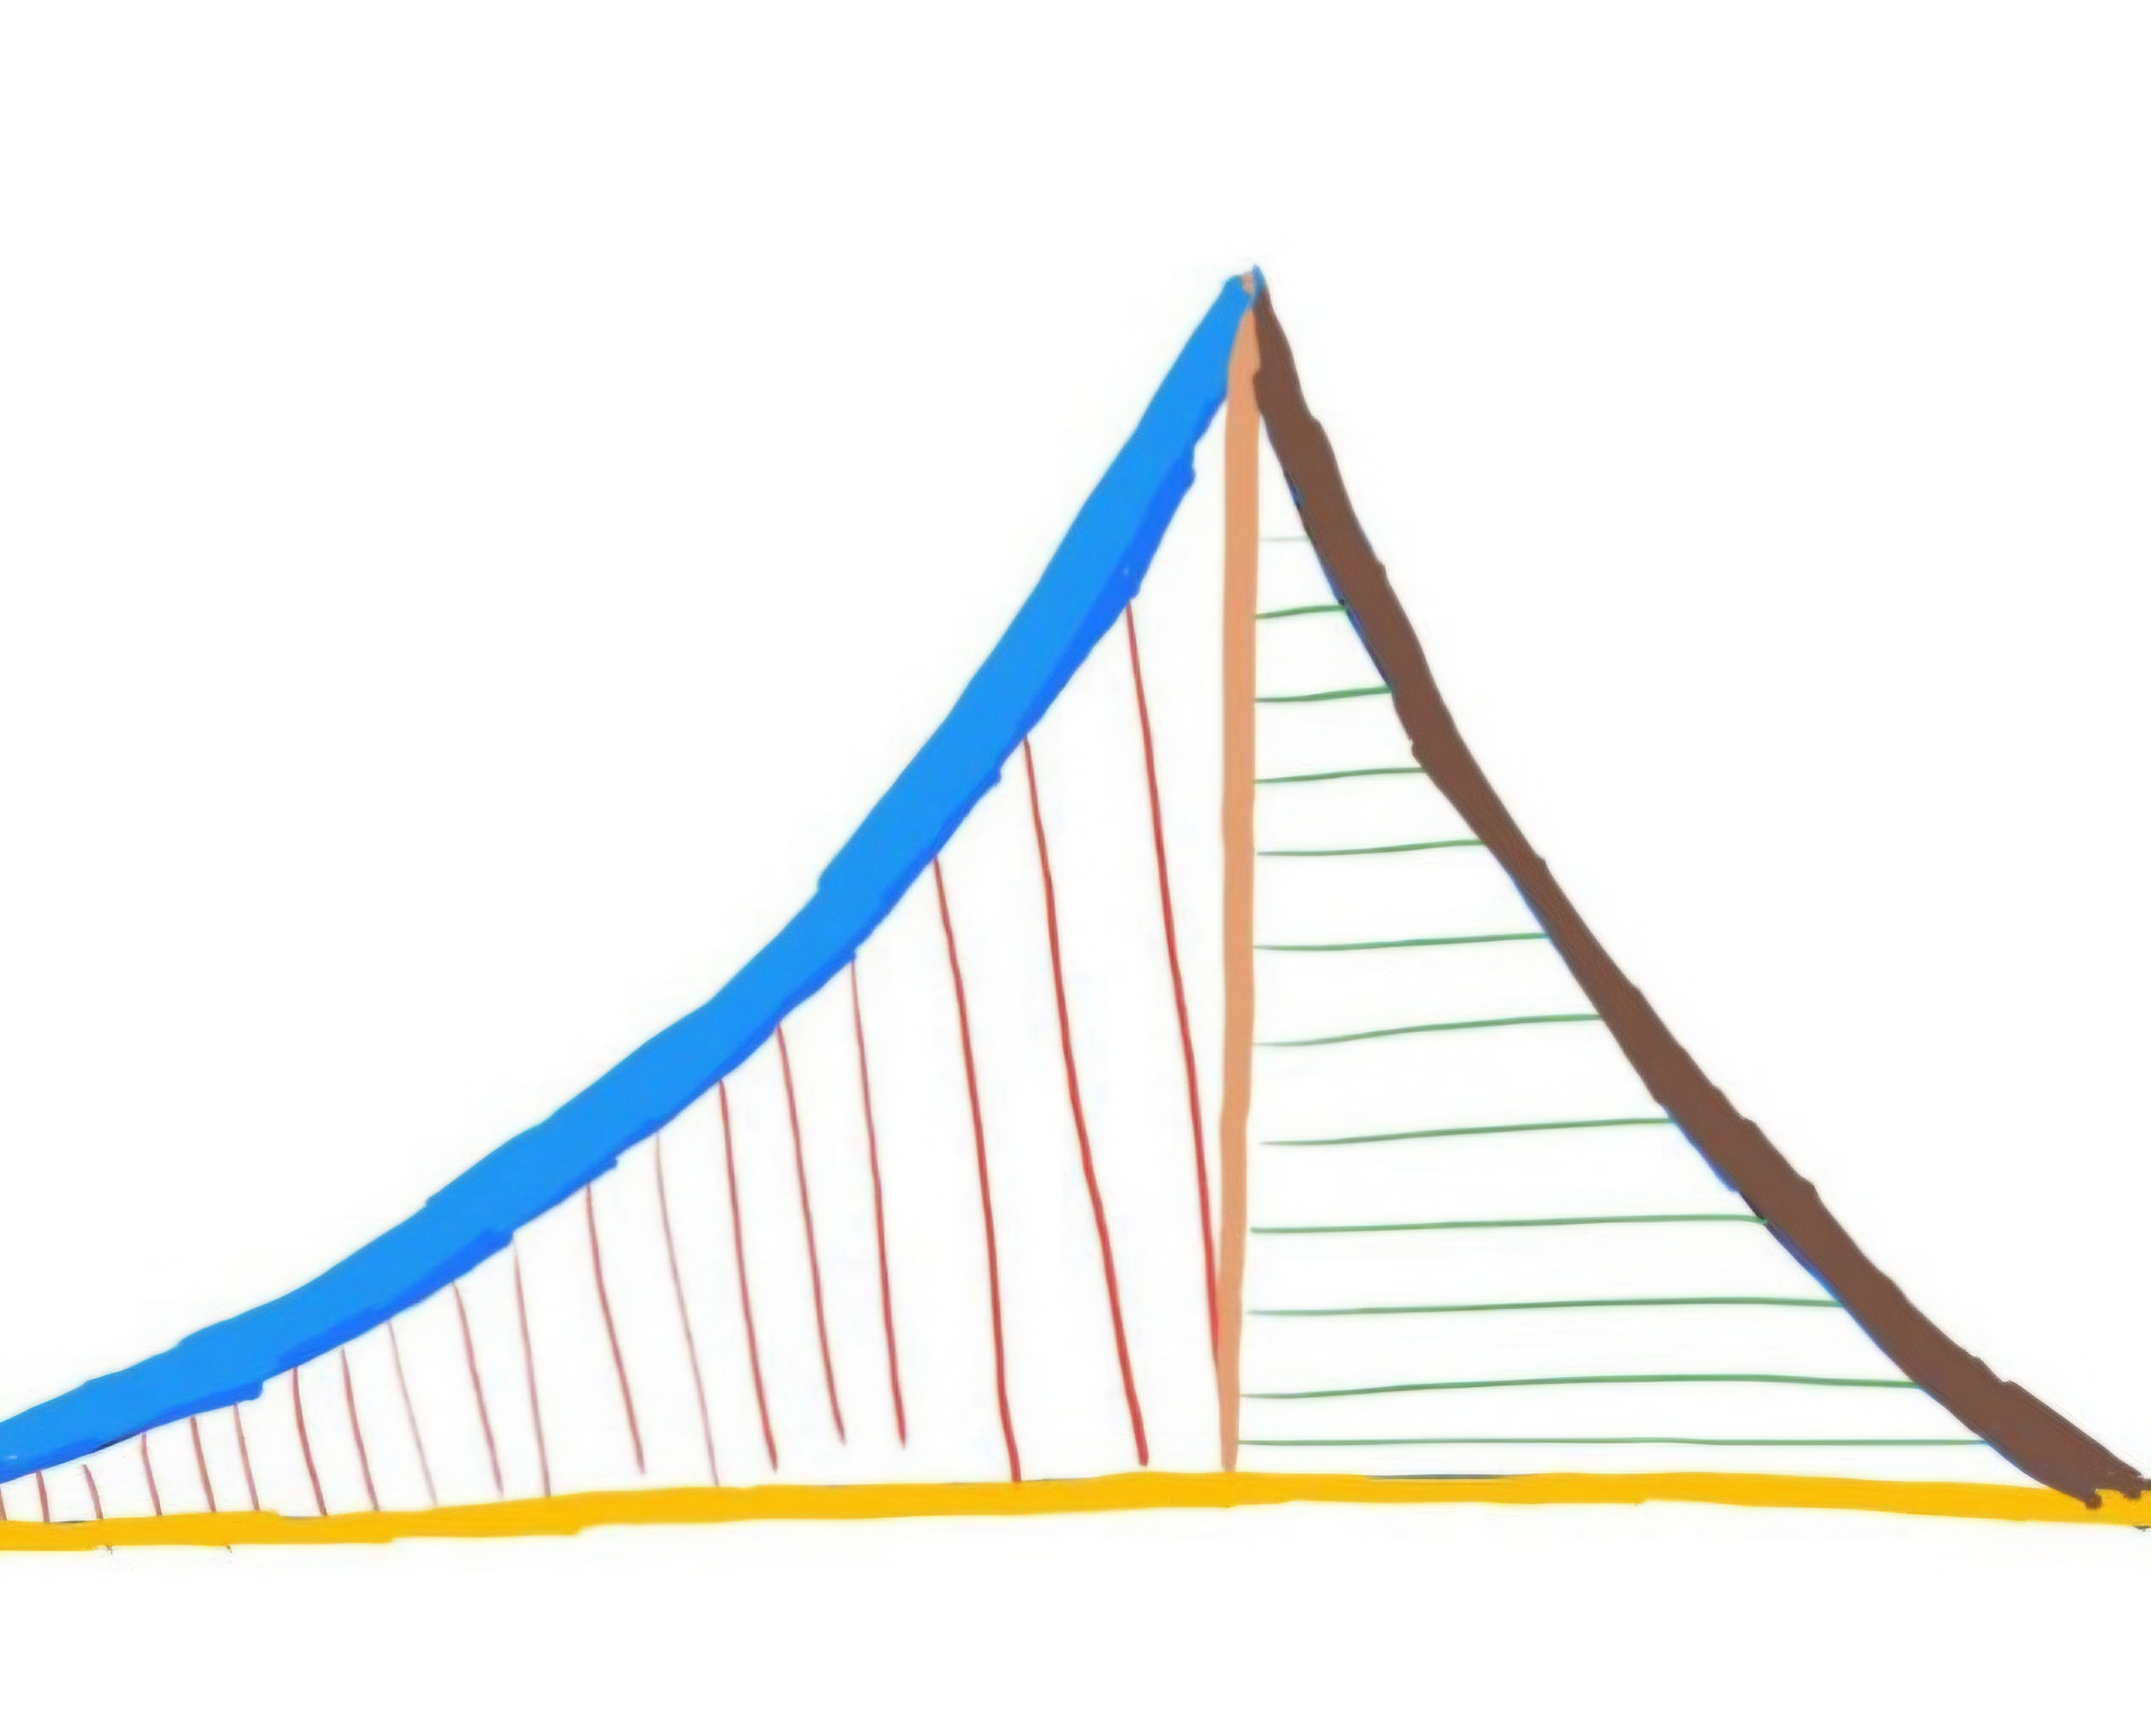
\includegraphics[width=0.2\columnwidth]{figs/logo.jpg}
\\
		{\huge	G. V. V. Sharma}\\Associate Professor,\\Department of Electrical Engineering, \\ IIT Hyderabad
	\end{center}
	%\end{flushleft}
%\IEEEpubid{\makebox[\columnwidth]{978-1-7281-5966-1/20/\$31.00 ©2020 IEEE \hfill} \hspace{\columnsep}\makebox[\columnwidth]{ }}
}
\maketitle

\newpage
\section*{About this Book}

This book introduces quadratic equations, complex numbers and other concepts in algebra.   
 All problems in the book are from NCERT mathematics textbooks from Class 9-12.  Exercises are from CBSE and JEE exam papers.   

There is no copyright, so readers are free to print and share.  

%This book is dedicated to my Hindi teacher in school, Shri Mandavi.
\begin{flushright}
\today
\end{flushright}
Github: https://github.com/gadepall/algebra
		\\
License: https://creativecommons.org/licenses/by-sa/3.0/
\\
and
\\
https://www.gnu.org/licenses/fdl-1.3.en.html

\newpage


\tableofcontents

\newpage
%\twocolumn
\onecolumn


%\renewcommand{\theequation}{\theenumi}
\numberwithin{equation}{enumi}
%\numberwithin{figure}{enumi}
\numberwithin{figure}{subsection}
%\renewcommand{\thefigure}{\theenumi}
\renewcommand{\thetable}{\theenumi}

\section{Identities}
\subsection{NCERT}
Verify
\begin{enumerate}[label=\thesubsection.\arabic*.,ref=\thesubsection.\theenumi,resume*]
	\item $x^3+y^3 = \brak{x+y}\brak{x^2-xy+y^2}$
	\item $x^3-y^3 = \brak{x-y}\brak{x^2+xy+y^2}$
	\item $x^3+y^3+z^3-3xyz = \frac{1}{2}\brak{x+y+z}\sbrak{\brak{x-y}^{2}+\brak{y-z}^{2}+\brak{z-x}^{2}}$
\end{enumerate}
Factorize each of the following
\begin{enumerate}[label=\thesubsection.\arabic*.,ref=\thesubsection.\theenumi]
	\item $8a^3+b^3+12a^2b+6ab^2$
	\item $8a^3-b^3-12a^2b+6ab^2$
	\item $27-125a^3-135a+225a^2$
	\item $64a^3-27b^3-144a^2b+108ab^2$
	\item $27p^3-\frac{1}{216}-\frac{9}{2}p^2 + \frac{p}{4}$
	\item $27y^3+125z^3$ 
	\item $64m^3-343n^3$
	\item $27x^3+y^3+z^3-9xyz$
\end{enumerate}
Find the value of each of the following 
\begin{enumerate}[label=\thesubsection.\arabic*.,ref=\thesubsection.\theenumi,resume*]
	\item $\brak{-12}^3+\brak{7}^3+\brak{5}^3$
	\item $\brak{28}^3+\brak{-15}^3+\brak{-13}^3$
\end{enumerate}
Give possible expressions for the length and breadth of each of the following rectangles, in which their areas are given
\begin{enumerate}[label=\thesubsection.\arabic*.,ref=\thesubsection.\theenumi,resume*]
	\item $25a^2-35a+12$
	\item $35a^2+13y-12$
\end{enumerate}
What are the possible expressions for the dimensions of the cuboids whose volumes are given below
\begin{enumerate}[label=\thesubsection.\arabic*.,ref=\thesubsection.\theenumi,resume*]
	\item $3x^2-12x$
	\item $12ky^2+8ky-20k$
\end{enumerate}

\section{Polynomials}
\subsection{NCERT}
\begin{enumerate}[label=\thesubsection.\arabic*, ref=\thesubsection.\theenumi,resume*]
%
\item Divide $p(x)$ by $g(x)$, where $p(x) = x + 3x^2– 1$ and $g(x) = 1 + x$.
\item Divide the polynomial $p(x) = 3x^4-4x^3-3x-1 $ by $x-1$.
\item Find the value of $k$, if $x – 1$ is a factor of $p(x) = 4x^3+ 3x^2 - 4x + k$.
%
\item Divide $2x^2+3x+1$ by $x+2$.
\item Divide $3x^3+x^2+2x+5$ by $1+2x+x^2$.
\item Find all the zeroes of $2x^4-3x^3-3x^2+6x-2$, if you know that two of its zeroes are $\sqrt{2}$ and $-\sqrt{2}$.
\item Find the remainder when $x^3-ax^2 +6x-a$ is divided by $x-a$.
\item Find the value of k, if x – 1 is a factor of p(x) in each of the following cases: 
\begin{enumerate}
\item $p(x) = x^2 + x + k$
\item $p(x) = kx^2-\sqrt{2}x+1$
\item $p(x) = 2x^2 + kx + \sqrt{2}$
\item $p(x) = kx^2  - 3x + k$
\end{enumerate}
\item Divide the polnyomial $p(x)$ by the polynomial $g(x)$ and find the quotient and remainder in each of the following:
\begin{enumerate}
\item $p(x) = x^3-3x^2+5x-3, g(x) = x^2-2$.
\item $p(x) = x^4-3x^2+4x+5, g(x) = x^2+1-x$.
\item $p(x) = x^4-5x+6, g(x) = 2-x^2$.
\end{enumerate}
\item Check whether the first polynomial is a factor of the second polynomial by dividing the second polynomial by the first polynomial:
\begin{enumerate}
\item $t^2-x,2t^4+3t^3-2t^2-9t-12$.
\item $x^2+3x+1, 3x^4+5x^3-7x^2+2x+2$.
\item $x^3-3x+1, x^5-4x^3+x^2+3x+1$.
\end{enumerate}
%
\item Obtain all the other zeroes of $3x^4+6x^3-2x^2-10x-5$, if two of its zeroes are $\sqrt{\frac{5}{3}}$and $-\sqrt{\frac{5}{3}}$.
\item On dividing $x^3-3x^2+x+2$ by a polynomial $g(x)$, the quotient and remainder were $x-2$ and $-2x+4$respectively.  Find $g(x)$.
\item Verify that the numbers given alongside the cubic polynomials below are their zeroes.  Also verify if the relationship between the zeroes and the coefficients in each case:
\begin{enumerate}
\item $2x^3+x^2-5x+2; \frac{1}{2}, 1, -2$
\item $x^3-4x^2+5x-2; 2, 1, 1$
\end{enumerate}
\item Find a cubic polynomial with the sum, sum of the product of its zeroes taken two at a time, and the product of its zeroes as 2, -7, -4 respectively.
\item If two zeroes of the polynomial $x^4-6x^3-26x^2+138x-35$ are $2\pm \sqrt{3}$, find the other zeroes.\item If the polynomial $x^4-6x^3+16x^2-25x+10$ is divided by another polynomial $x^2-2x+k$, the remainder comes out to be $x+a$, find $k$ and $a$.

\end{enumerate}

\section{Roots}
\subsection{NCERT}
Find the roots of the following equations graphically or otherwise.
\begin{enumerate}[label=\thesubsection.\arabic*, ref=\thesubsection.\theenumi]
	\begin{multicols}{2}
	\item $x^2-2x=0$
	\item $x^3-x^2+2=0$
	\item $x^5-x^4+3=0$
	\item $2-y^2-y^3+2y^8=0$
	\item $x-x^3=1$
	\item $5x^3+4x^2+7x=0$
	\item $4-y^2=0$
	\item $x^2+x+2 = 0$
	\item $4x^2-3x+7 = 0$
	\item $y^2+\sqrt{2} = 0$
	\item $3\sqrt{t}+t\sqrt{2} = 1$
	\item $y+\frac{2}{y} = 1$
	\item $x^2+x = 1$
	\item $y+{y}^2+4 = 0$
	\item $y(x)=5x^2-3x+7 = 0$.  Find $y(1).$
	\item $3y^3-4y+\sqrt{11}=0$.  Find $y(2).$
	\item $4t^4+5t^3-t^2+6=0$
	\item $5x^3-2x^2+3x-2=0$.  Find $y(1), y(0)$ and $y(-1)$.
	\item $5x-4x^2+3=0$.  Find $y(2), y(0)$ and $y(-1)$.
	\item $\brak{x-2}^2+1 = 2x-3$
	\item $x\brak{2x+3} = x^2+1$
	\item $\brak{x+2}^3 = x^3-4$
	\item $\brak{x+1}^2 = 2\brak{x-3}$
	\item $x^2-2x = -2\brak{3-x}$
	\item $\brak{2x-1}\brak{x-3} = \brak{x+5}\brak{x-1}$
	\item $\brak{x+2}^{3} = 2x\brak{x^2-1}$
	\item ${x}^{3}-4x^2-x+1 = \brak{x-2}^3$
	\item $2{x}^{2}-5x+3 = 0$
	\item $6{x}^{2}-x-2 = 0$
	\item $3{x}^{2}-2\sqrt{6}x+2 = 0$
	\item ${x}^{2}-3x-10 = 0$
	\item $2{x}^{2}+x-6 = 0$
	\item $\sqrt{2}{x}^{2}+7x+5\sqrt{2} = 0$
	\item $2{x}^{2}-x+\frac{1}{8} = 0$
	\item $100{x}^{2}-20x+1 = 0$
	\item $5{x}^{2}-6x-2 = 0$
	\item $4{x}^{2}+3x+5 = 0$
	\item $3{x}^{2}-5x+2 = 0$
	\item ${x}^{2}+4x+5 = 0$
	\item $2{x}^{2}-2\sqrt{2}x+1 = 0$
	\item $x+\frac{1}{x}=3, x\neq{0}$
\item $\frac{1}{x}-\frac{1}{x-2} = 3, x\neq 0,2$
\item $3x^2-2x+\frac{1}{3} = 0$. 
\item $x^2-4x+3 = 0$.
\item $2x^2-4x+3 = 0$.
\item $x-\frac{1}{x}=3, x\neq{0}$
\item
$\frac{1}{x+4}-\frac{1}{x-7}=\frac{11}{30}, x\neq{-4,7}$
\item $2x^2-3x+5=0$
\item $3x^2-4 \sqrt 3x+4=0$
\item $2x^2-6x+3=0$
	\end{multicols}
\end{enumerate}
Find $p(0), p(1)$ and $p(2)$ for each of the following polynomials.
\begin{enumerate}[label=\thesubsection.\arabic*, ref=\thesubsection.\theenumi,resume*]
	\begin{multicols}{2}
	\item $p(y)=y^2-y+1$
	\item $p(t)=2+t+2t^2-t^3$
	\item $p(x)=x^3$
	\item $p(x)=\brak{y-1}\brak{y+1}$
	\end{multicols}
\end{enumerate}
Find the values of $k$ for each of the following quadratic equations, so that they have two equal roots
\begin{enumerate}[label=\thesubsection.\arabic*, ref=\thesubsection.\theenumi,resume*]
\item 	$2x^2+kx+3 = 0$
\item 	$kx\brak{x-2}+6= 0$
\end{enumerate}
Verify whether the following are zeroes of the polynomial, indicated against them.
\begin{enumerate}[label=\thesubsection.\arabic*, ref=\thesubsection.\theenumi,resume*]
	\item $p(x) = x^2-1, \quad x=-1, 1$.
	\item $p(x) = \brak{x-2}\brak{x+1}, \quad x=-1, 2$.
	\item $p(x) = 3x^2-1, x=-\frac{1}{\sqrt{3}},\frac{2}{\sqrt{3}}$.
\end{enumerate}

\section{Quadratic Equations}
\subsection{NCERT}
\begin{enumerate}[label=\thesubsection.\arabic*,ref=\thesubsection.\theenumi]
%
	\item Janak and Jivanti together have 45 marbles. Both of them lost 5 marbles each, and the product of the number of marbles they now have is 124. We would like to find out how many marbles they had to start with.
\item  A cottage industry produces a certain number of toys in a day. The cost of production of each toy (in rupees) was found to be 55 minus the number of toys produced in a day. On a particular day, the total cost of production was \rupee 750. We would like to find out the number of toys produced on that day.
\item The product of Sunita’s age (in years) two years ago and her age four years from now is one more than twice her present age. What is her present age?
\item Find two consecutive odd positive integers, sum of whose squares is 290.
\item A motor boat whose speed is 18 km/h in still water takes 1 hour more to go 24 km upstream than to return downstream to the same spot. Find the speed of the stream.
%
\item The product of two consecutive positive integers is 306. We need to find the integers.
\item Rohan’s mother is 26 years older than him. The product of their ages (in years) 3 years from now will be 360. We would like to find Rohan’s present age.
\item A train travels a distance of 480 km at a uniform speed. If the speed had been 8 km/h less, then it would have taken 3 hours more to cover the same distance. We need to find the speed of the train.
\item Find two numbers whose sum is 27 and product is 182. 
\item  Find two consecutive positive integers, sum of whose squares is 365. 
\item  A cottage industry produces a certain number of pottery articles in a day. It was observed on a particular day that the cost of production of each article (in rupees) was 3 more than twice the number of articles produced on that day. If the total cost of production on that day was \rupee 90, find the number of articles produced and the cost of each article.\item The sum of the reciprocals of Rehman’s ages, (in years) 3 years ago and 5 years from now is $\frac{1}{3}$.  Find his present age.
\item In a class test, the sum of Shefali’s marks in Mathematics and English is 30. Had she got 2 marks more in Mathematics and 3 marks less in English, the product of their marks would have been 210. Find her marks in the two subjects.
\item The difference of squares of two numbers is 180. The square of the smaller number is 8 times the larger number. Find the two numbers.
\item A train travels 360 km at a uniform speed. If the speed had been 5 km/h more, it would have taken 1 hour less for the same journey. Find the speed of the train.
\item Two water taps together can fill a tank in 9$\frac{3}{ 8}$
hours. The tap of larger diameter takes 10
hours less than the smaller one to fill the tank separately. Find the time in which each tap can separately fill the tank.
\item An express train takes 1 hour less than a passenger train to travel 132 km between Mysore and Bangalore (without taking into consideration the time they stop at intermediate stations). If the average speed of the express train is 11km/h more than that of the passenger train, find the average speed of the two trains.
\item Sum of the areas of two squares is 468 $m^22$ find the sides of the two squares.
\item Is the following situation possible? If so, determine their present ages. The sum of the ages of two friends is 20 years. Four years ago, the product of their ages in years was 48.
%
\end{enumerate}

\iffalse
\subsection{Formulae}
\begin{enumerate}[label=\thesubsection.\arabic*,ref=\thesubsection.\theenumi]
	\item Find the sum
\begin{align}
	\label{eq:ap-sum10}
	S = 1 + 2 + \dots + 10
\end{align}
\solution Reversing the sum in
	\eqref{eq:ap-sum10}
	as
\begin{align}
	\label{eq:ap-sum10-rev}
	S = 10 + 9 + \dots + 1
\end{align}
and adding 
	\eqref{eq:ap-sum10}
	and
	\eqref{eq:ap-sum10-rev},
\begin{align}
	\label{eq:ap-sum10-add}
	2S &= 11 + 11 + \dots + 11 \quad 10 \text{ times}
	\\
	\implies S &= \frac{11 \times 10}{2} = 55
\end{align}
\item The sum of the first $n$ natural numbers is
\begin{align}
	\sum_{k=1}^{n}k &= 1+ 2 + \dots + n
	\\
	&= \frac{n\brak{n+1}}{2}
	\label{eq:ap-sumn}
\end{align}
\item The $n^{th}$ term of an arithmetic progression (AP) is
\begin{align}
	\label{eq:ap-nthterm}
	x(n) = x(0) + nd, \quad n = 0, 1, \dots
\end{align}
\item 
\begin{align}
	\label{eq:ap-nsum}
	 y(n)=\sum_{k=0}^{n}x(k) = \frac{n+1}{2}\brak{x(0) + \frac{dn}{2}}
\end{align}
\solution
From
	\eqref{eq:ap-nthterm}
	and
	\eqref{eq:ap-nsum},
\begin{align}
	\label{eq:ap-nthsum}
	 \sum_{k=0}^{n}x(k) &= 
\sum_{k=0}^{n}
	 \brak{x(0) + kd} 
	 \\
	 &= 
\sum_{k=0}^{n}x(0) + 
d\sum_{k=1}^{n}k
	  = \brak{n+1}x(0) + d\frac{n\brak{n+1}}{2}
\end{align}
upon substituting from
	\eqref{eq:ap-sumn}, yielding
	\eqref{eq:ap-nthsum}
	upon simplification.
\end{enumerate}

\subsection{CBSE}
\begin{enumerate}[label=\thesubsection.\arabic*,ref=\thesubsection.\theenumi,itemsep=1pt]
 \item In an AP, if $d=2, n=5$ and $a_n=0$, then value of $a$ is
    \hfill (10,  2011)
\begin{multicols}{4}
    \begin{enumerate}
         \item 10
         \item 5
         \item -8
         \item 8
    \end{enumerate}
\end{multicols}
 \item Find whether -150 is a term of the AP: $17, 12, 7, 2,\dots$?
    \hfill (10,  2011) \item Find the value of the middle term of the following AP: $- 6, -2, 2,\dots, 58.$
   \hfill (10,  2011) \item Determine the AP whose fourth term is 18 and the difference of the ninth term from the fifteenth term is 30.
\hfill (10,  2011) \item Find how many two-digit numbers are divisible by $6$.
 How many multiples of $4$ lie between $10$ and $250$ ? Also find their sum.
    \hfill (10,  2011)
         \item The ratio of the $11\textsuperscript{th}$ term to $17\textsuperscript{th}$ term of an AP is $3:4$. Find the ratio of $5\textsuperscript{th}$ to $21\textsuperscript{th}$ of the same AP. Also, find the ratio of the sum of first $5$ terms to that of first $21$ terms
        \hfill (10,  2023) \item $250$ logs are stacked in the following manner:
        $22$ logs in the bottom row, $21$ in the next row, $20$ in the row next to it and so on. In how many rows are the $250$ logs placed and how many logs are there in top row ?
\hfill (10,  2023)
 \item If $-\frac{5}{7}$, $a$, $2$ are consecutive terms in an Arthimetic Progression, then the value of $a$ is 
    \hfill (10,  2022)
    \begin{multicols}{4}
\begin{enumerate}    
\item $\frac{9}{7}$
 \item $\frac{9}{14}$
 \item $\frac{19}{7}$
 \item $\frac{19}{14}$
    \end{enumerate}
\end{multicols}
 \item Find the sum of first $16$ terms of an Arithmetic Progression whose $4^{\text{th}}$ and $9^{\text{th}}$ terms are $-15$ and $-30$ respectively.
        \hfill (10,  2022) \item If the sum of first $14$ terms of an Arithmetic Progression is $1050$ and its fourth term is $40$, find its $20^{\text{th}}$ term.
\hfill (10,  2022)
         \item Find the sum of the first twelve $2$-digit numbers which are 
multiples of $6$.
\hfill (10,  2022)
         \item In an AP, if $a_2=26$ and $a_{15} = -26$, then write the AP.
\hfill (10,  2022)
         \item In Mathematics, relations can be expressed in various ways. The 
matchstick patterns are based on linear relations. Different strategies 
can be used to calculate the number of matchsticks used in different 
		\figref{fig:ap} 
One such pattern is shown below. Observe the pattern and answer the 
following questions using Arithmetic Progression 

    \hfill (10,  2022) 
\begin{figure}[H]
    \centering
	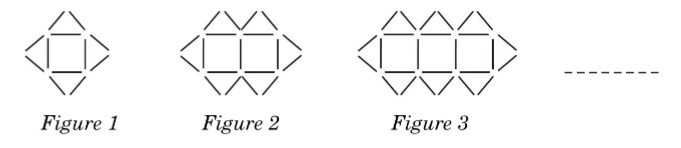
\includegraphics[width=\columnwidth]{figs/ap/ap.jpg}
	\caption{}
    \label{fig:ap}
\end{figure}
    \begin{enumerate}
	 \item Write the AP for the number of triangles used in the \figref{fig:ap}. Also, 
write the nth term of this AP.
 \item Which figure has $61$ matchsticks ? 
    \end{enumerate} 
 \item In an AP if the sum of third and seventh term is zero, find its $5^{\text{th}}$ term.
        \hfill (10,  2022)
  \item Determine the AP whose third term is $5$ and seventh term is $9$.
        \hfill (10,  2022) \item Find the sum of the first $20$ terms of an AP whose $n^{\text{th}}$ term is given as $a_n=5-2n$

%
        \hfill (10,  2022) \item Find the common difference $d$ of an AP whose first term is $10$ and the sum of the first $14$ terms is $1505$.
        \hfill (10,  2022) \item For what value of $n$, are the $n^{\text{th}}$ terms of the APs: $9,7,5,\dots$ and $15,12,9,\dots$ the same?
    \hfill (10,  2022)
	 \item Write the common difference of the AP: $\frac{1}{5}, \frac{4}{5}, \frac{7}{5}, \frac{10}{5}, \cdots$
	\hfill (10,  2021) \item Find the $8^{th}$ term of the AP whose first term is $-2$ and common difference is $3$.

%
	\hfill (10, 2021) \item
	Roshini being a plant lover decides to start a nursery. She bought few plants with pots. She placed the pots in such a way that the number of pots in the first row is $2$, in the second is $5$, in the third row is $8$ and so on as shown in 
			\figref{fig:Plants}.
		\begin{figure}[H]
			\centering	
			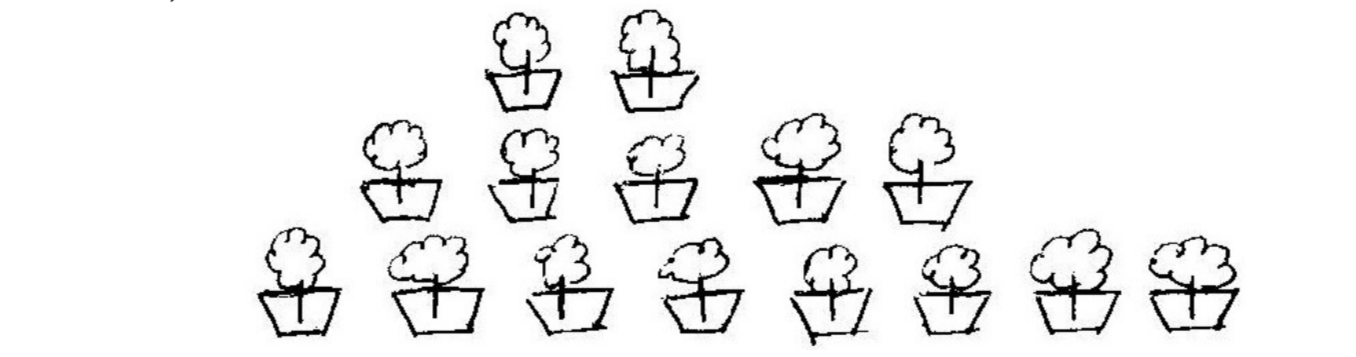
\includegraphics[width=\columnwidth]{figs/ap/Plant.png}
			\caption{}
			\label{fig:Plants}
		\end{figure}
		Based on the above, answer the following questions 
\hfill (10, 2021)
		\begin{enumerate}
\item How many pots were placed in the $7^{th}$ row ?
				\begin{multicols}{4}
\begin{enumerate}    
					 \item $20$
					 \item $23$
					 \item $77$
					 \item $29$
				\end{enumerate}
\end{multicols}
 \item If Roshini wants to place $100$ pots in total, then total number of rows formed in the arrangement will be ?
				\begin{multicols}{4}
\begin{enumerate}    
					 \item $8$
					 \item $9$
					 \item $10$
					 \item $12$
				\end{enumerate}
\end{multicols}
 \item How many pots are placed in the last row ?
				\begin{multicols}{4}
\begin{enumerate}    
					 \item $20$
					 \item $23$
					 \item $26$
					 \item $29$
				\end{enumerate}
\end{multicols}
			 \item If Roshini has sufficient space for $12$ rows, then how many total number of pots are placed by her wih the same arrangement ?
				\begin{multicols}{4}
\begin{enumerate}    
					 \item $222$
					 \item $155$
					 \item $187$
					 \item $313$
				\end{enumerate}
\end{multicols}
		\end{enumerate} 
	 \item The sum of the first $4$ terms of an AP is zero and its $4^{th}$ term is $2$. Find the AP.

	\hfill (10, 2021) \item If the sum of the first $n$ terms of an AP is given by $S_n = 4n - n^2$, then find its $n^{th}$ term. Hence, find the $25^{th}$ term and the sum if the first 25 terms of this AP.

\hfill (10, 2021)
	 \item Find the mean of first $10$ composite numbers.
	\hfill (10, 2021) \item If $S_n$ denotes the sum of first $n$ terms of an AP, prove that $S_{12} = 3(S_8 - S_4)$.

%
	\hfill (10, 2021) \item After how many decimal places will the decimal expansion of the rational number $\frac{14587}{1250}$ terminate ?			
\hfill (10, 2021)
	 \item If the $6^{th}$ and $14^{th}$ terms of an AP are 29 and 69 respectively, then find the $10^{th}$ term of the AP.
	\hfill (10, 2021) \item If the first three consecutive terms of an AP are $3y-1, 3y+5$ and $5y+1$ find the value of $y$. 
\hfill (10, 2021)
 \item Which of the following is not an AP? 
\hfill (10, 2020)
\begin{multicols}{2}
\begin{enumerate}    
               \item $-1.2,0.8,2.8,\dots$ 
	        \item $3,3+\sqrt2,3+2\sqrt2,3+3\sqrt2,\dots$ 
	        \item $\frac{4}{3},\frac{7}{3},\frac{9}{3},\frac{12}{3},\dots$ 
	        \item $\frac{-1}{5},\frac{-2}{5},\frac{-3}{5},\dots$ 
\end{enumerate}
\end{multicols}
 \item Find the sum of the first $100$ natural numbers.	
	\hfill (10, 2020)
 \item Find the sum
\hfill (10, 2020)
\begin{align*}
	\brak{-5} + \brak{-8} + \brak{-11} + \dots + \brak{-230}
\end{align*}
 \item Find the number of terms in the AP 
    $18,15\frac{1}{2},13, \dots, 47.$
\hfill (10, 2019) \item Determine the AP whose third term is $16$ and $7^{th}$ term exceeds the $5^{th}$ term by $12$.

%
\hfill (10, 2019) \item Find the value of $x$, when in the AP given below
\hfill (10, 2019)
\begin{align*}
2 + 6 + 10 + \dots + x = 1800.    
\end{align*}
 \item Which term of the AP $-4, - 1, 2, \dots$ is $ 101$?
\hfill (10, 2019) \item In an AP, the first term is $- 4$, the last term is $29$ and the sum of all its terms is $150$. Find its common difference.
\hfill (10, 2019) \item Find the $21^{st}$ term of the AP $-4 \frac{1}{2},-3,-1\frac{1}{2}, \dots $
\hfill (10, 2019) \item Find the common difference of the AP 
\hfill (10, 2019)
\begin{align*}
\frac{1}{a} , \frac{3-a}{3a},\frac{3-2a}{3a} , \dots (a \neq 0)
\end{align*}
 \item Which term of the Arithmetic Progression $-7, -12, -17, -22, \dots$ will be $-82$? Is $-100$ any term of the AP? Give reason for your answer.
\hfill (10, 2019) \item How many terms of the Arithmetic Progression $45, 39, 33,  \dots  $ must be taken so that their sum is $180$ ? Explain the double answer.
\hfill (10, 2019) \item Find after how many places of decimal the decimal form of the number $\frac {27}{2^35^43^2}$ will terminate.
\hfill (10, 2019) \item Find the sum of first $10$ multiples of $6$

\hfill (10, 2019) \item If $m$ times the $m^{th}$ term of an Arithmetic Progression is equal to $n$ times
its $n^{th}$ term and $m \neq n$, show that the $\brak{m + n}^{th}$ term of the A.P is zero
\hfill (10, 2019) \item The sum of the first three numbers in an Arithmetic Progression is $18$. If the product of the first and the third term is $5$ times the common
difference, find the three numbers.
 \item Find the sum of all the two digit numbers which leave the remainder $2$ when divided by $5$.
\hfill (10, 2019) \item If in an AP, $a=15$, $d=-3$ and $a_n=0$, then find the value of $n$.
\hfill (10, 2019) \item If ${S_n}$, the sum of the first ${n}$ terms of an AP is given by ${S_n = 2n^2 + n}$, then find its $n^{th}$ term. 
\hfill (10, 2019) \item If the $17^{th}$ term of an AP exceeds its $10^{th}$ term by $7$, find the common difference.

\hfill (10, 2019) \item If the sum of the first $p$ terms of an AP is $q$ and the sum of the first $q$ terms is $p$, then show that the sum of the first $\brak{p + q}$ terms is $\cbrak {-\brak {p + q}}$.
%
\hfill (10, 2019) \item Write the common difference of the AP${\sqrt3} , {\sqrt12} , {\sqrt27} , {\sqrt48}$ ,  \dots  
%
\hfill (10, 2019) \item In an AP, the $n^{th}$ term is ${\frac{1}{m}}$ and the $m^{th}$ term is $\frac{1}{n}$. Find 
\hfill (10, 2019)
\begin{enumerate}
      \item  $\brak{mn}^{th}$ term,
      \item sum of first $\brak{mn}$ terms.
\end{enumerate}
%
 \item The first term of an AP is 3, the last term is 83 and the sum of all its terms is 903. Find the number of terms and the common difference of the AP.
 \hfill (10, 2019) \item If the sum of first $n$ terms of an  AP  is $n^2$, then find its $10^{th} $term.
\hfill (10, 2019) \item Which term of the AP: $3, 15, 27, 39, \dots$ will be $120$ more than its $21$st term?

\hfill (10, 2019) \item If $S_n$, the sum of first $n$ terms of an  AP  is given by $S_n=3n^2-4n$, find the $n^{th}$ term.

\hfill (10, 2019) \item If the sum of first four terms of an  AP  is $40$ and that of first $14$ terms is $280$. Find the sum of its first $n$ terms.
\hfill (10, 2019)
%
			 \item In an  AP , if the common difference $d = -4$, and the seventh term $a_7$ is $4$, then find the first term.		
			\hfill (10, 2018) \item The sum of four consecuive numbers in an AP is $32$ and the ratio of the product of the first and the last term to the product of two middle term is $7:15$. Find the numbers.
	\hfill (10, 2018) \item Find the sum of $8$ multiples of $3$.
\hfill (10, 2018)
%
			 \item In an  AP , if the common difference $d = -4$, and the seventh term $a_7$ is $4$, then find the first term.		
			\hfill (10, 2018) \item The sum of four consecuive numbers in an AP is $32$ and the ratio of the product of the first and the last term to the product of two middle term is $7:15$. Find the numbers.
%
	\hfill (10, 2018) \item Find the sum of $8$ multiples of $3$.
\hfill (10, 2018)
 \item The $5^{th}$ and $15^{th}$ terms of an AP are $13$ and $-17$ respectively. Find the sum of first $21$ terms of the AP.
\hfill (10, 2018)
%
 \item The sum of the first $n$ terms of an AP is $5n^{2}+3n$. If its $m^{th}$ terms is $168$, find the value of $m$. Also find the $20^{th}$ term of the AP.
\hfill (10, 2018) \item The $4^{th}$ and the last terms of an AP are $11$ and $89$ respectively. If there are $30$ terms in the AP, find the A.P and its $23^{rd}$ term.
\hfill (10, 2018) \item Write the $m^{th}$ term of the AP $$\frac{1}{k},\dfrac{1+k}{k},\dfrac{1+2k}{k},\dots$$
\hfill (10, 2018)
 \item Which term of the AP: $8,14,20,26,\dots$ will be $72$ more than its $41^{st}$ term ?

\hfill (10, 2017) \item If the $10^{th}$ term of an AP is $52$ and the $17^{th}$ term is $20$ more than the $13^{th}$ term, find the AP
\hfill (10, 2017) \item If the ratio of the sum of the first n terms of two A.Ps is $\brak{7n + 1}$ : $\brak{4n + 27}$, then find the ratio of their $9^{th}$ terms.
\hfill (10, 2017) \item For what value of $n$, are the $n^{th}$ terms of two APs $63,65,67,\dots$ and $3,10, 17,\dots$ equal?
\hfill (10, 2017) \item How many terms of an AP: $9,17,254,\dots$ must be taken to  give a sum of $636$?

\hfill (10, 2017) \item What is the common difference of an A.P in which $a_{21} - a_7 = 84$ ?
\hfill (10, 2017) \item Which term of the progression $20,19\frac{1}{4},18\frac{1}{2},17\frac{3}{4},\dots$ is the first negative term ?

\hfill (10, 2017) \item The first term of an AP is $5$, the last term is $45$ and the sum of all its terms is $400$. Find the number of terms and the common difference of the AP.
\hfill (10, 2017)
 \item For what value of $k$ will $k+9, 2k-1$ and $2k+7$ are the consecutive terms of an AP ?
 \hfill (10, 2016) \item  The $4^{th}$ term of an AP is zero. Prove that the $25^{th}$ term of the AP is three times its $11^{th}$ term.
 \hfill (10, 2016) \item  If the ratio of the sum of first $n$ terms of two APs is $\brak{7n + 1} : \brak{4n + 27}$, find the ratio of their $m^{th}$ terms.
\hfill (10, 2016) \item The sums of first $n$ terms of three arithmetic progressions are $S_1, S_2$ and $S_3$ respectively. The first term of each AP is $1$ and their common differences are $1, 2$ and $3$ respectively. Prove that $S_1+S_3=S_2$.

\hfill (10, 2016) \item The digits of a positive number of three digits are in AP and their sum is $15$. The number obtained by reversing the digits is $594$ less than the original number. Find the number.
\hfill (10, 2016) \item The houses in a row are numbered consecutively from $1$ to $49$. Show that there exists a value of $X$ such that sum of numbers of houses preceeding the house numbered $X$ is equal to sum of the numbers of houses following $X$.
\hfill (10, 2016)
 \item In an AP, if $S_5 + S_7$ = $167$ and $S_10$ = $235$, then find the AP, where $S_n$ denotes the sum of its first n terms.
\hfill (10, 2015) \item The $14^{th}$ term of an AP is twice its $8^{th}$ term. If its $6^{th}$ term is – $8$, then find the sum of its first $20$ terms.
\hfill (10, 2015) \item Find the $60^{th}$ term of the AP $8, 10,  12,  \dots ,$ if it has a total of 60 terms and hence find the sum of its last $10$ terms.
\hfill (10, 2015) \item The $16^{th}$ term of an {AP} is five times its third term. If its $10^{th}$ term is $41$, then find the sum of its first fifteen terms.
\hfill (10, 2015)
 \item An arithmetic progression $5, 12, 19,  \dots $ has $50$ terms. Find its last term. Hence find the sum of its last $15$ terms.
%
\hfill (10, 2015) \item The $13^{th}$ term of an AP is four times its $3^{rd}$ term. If its fifth term is $16$, then find the sum of its first ten terms.
\hfill (10, 2015)
 \item If the $n^{th}$ term of an AP is $\brak{2n+1}$, then sum of its first three terms is 
\hfill (10, 2012)
\begin{multicols}{4}
\begin{enumerate}
 \item $6n + 3$ 
 \item $15$ 
 \item $12$ 
 \item $21$ 
\end{enumerate}
\end{multicols}
 \item The next term of AP: $\sqrt {18}, \sqrt {50}, \sqrt {98}, \dots$ is \hfill (10, 2012)
\begin{multicols}{4}
\begin{enumerate}
 \item $\sqrt {146}$ 
 \item $\sqrt {128}$ 
 \item $\sqrt {162}$ 
 \item $\sqrt {200}$ 
\end{enumerate}
\end{multicols}
%discrete
 \item Find the common difference of an AP whose first term is $5$ and the sum of its first four terms is half the sum of the next four terms. 
%discrete
 \hfill (10, 2012) \item The $17th$ term of an AP is $5$ more than twice its $8^{th}$ term. If the $11th$ term of the AP is $43$, then find the $n^{th}$ term. 
%
\hfill (10, 2012) \item Sum of the first $14$ terms of an  AP  is $1505$ and its first term is $10$. Find its $25^{th}$ term. 
\hfill (10, 2012) \item In an  AP , the first term is $12$ and the common difference is $6$. If the last term of the  AP  is $252$, find its middle term. 
\hfill (10, 2012) \item If $4$ times the fourth term of an  AP  is equal to $18$ times its $18^{th}$ term, then find its $22^{th}$ term. 
\hfill (10, 2012) \item The sum of $4^{th}$ and $8^{th}$ term terms of an  AP  is $24$ and the sum of its $6^{th}$ and $10^{th}$ terms is $44$. Find the sum of first ten terms of the  AP  
\hfill (10, 2012)
\item In an AP, if $d=2, n=5$ and $a_n=0$, then value of $a$ is
    \hfill (10, 2011)
    \begin{multicols}{4}
\begin{enumerate}
%
\item 10
%
\item 5
%
\item -8
%
\item 8
    \end{enumerate}
\end{multicols}
\item Find whether -150 is a term of the AP: $17, 12, 7, 2,\dots$?
    \hfill (10, 2011)
\item Find the value of the middle term of the following AP: $- 6, -2, 2,\dots, 58.$
   \hfill (10, 2011)
\item Determine the AP whose fourth term is 18 and the difference of the ninth term from the fifteenth term is 30.
    \hfill (10, 2011)
\item
	{Assertion ($A$):} $a,b,c$ are in  AP  if and if only if $2b = a + c$.
%
{Reason($R$):} The sum of first $n$ natural numbers is $n^2$.
\hfill (10, 2023)
\begin{enumerate}
\item Both Assertion $\brak{A}$ and Reason $\brak{R}$ are true and Reason $\brak{R}$ is the correct explanation of Assertion $\brak{A}$.
\item Both Assertion $\brak{A}$ and Reason $\brak{R}$ are true and Reason $\brak{R}$ is not the correct explanation of Assertion $\brak{A}$.
\item Assertion $\brak{A}$ is true but Reason $\brak{R}$ is false.
\item Assertion $\brak{A}$ is false but Reason $\brak{R}$ is true.
\end{enumerate}
\item
How many terms are there in  AP  whsoe first and fifth term are $-14$ and $2$, respectively and the last term is $62$.
\hfill (10, 2023)
\item
Which term of the AP: $65,61,57,53, \dots$ is the first negative term?
\hfill (10, 2023)
\item Three bells ring at intervals of  6, 12 and 18 minutes. If all the three bells rang at  6 a.m., when will they ring together again ?
\hfill (10, 2023)
\item For what value of $k$ will $(k+9), (2k-1)$ and $( 2k+7)$ be consecutive terms of an AP?

\hfill (10, 2016)
\item The sums of the first $n$ terms of three arithmetic progressions are $S_0, S_2$ and $S_3$ respectively. The first term of each AP is $1$ and their common differences are $1, 2$ and $3$ respectively. Prove that $S_1 + S_3 = 2S_2$.
								\hfill (10, 2016)
\item The $5^{\text{th}}$ term of an Arithmetic Progression (AP) is 26 and the 10th term is 51. Determine the $15^{\text{th}}$ term of the AP.
    \hfill (10, 2006)
\item Find the sum of all the natural numbers less than 100 which are divisible by 6.

    \hfill (10, 2006)
\item Find how many two-digit numbers are divisible by $6$.
    \hfill (10, 2011)
\item  How many multiples of $4$ lie between $10$ and $250$ ? Also find their sum.
    \hfill (10, 2011)
\item The sum of first 20 odd natural numbers is : 
    \hfill (10, 2012)
    \begin{multicols}{4}
\begin{enumerate}
\item $100$ 
\item $210$ 
\item $400$ 
\item $420$ 
\end{enumerate}
\end{multicols}
\item How many two-digit numbers are divisible by 3? 
    \hfill (10, 2012)
\item Find the sum of all multiples of 7 lying between $500$ and $900$. 
    \hfill (10, 2012)
\item Find the sum of all three digit natural numbers, which are multiples of $11$. 
    \hfill (10, 2012)
\item Find the sum of first 40 positive integers divisible by $6$. 
    \hfill (10, 2012)
\item How many multiples of $4$ lie between $10$ and $205$?   
    \hfill (10, 2019)
\item Find the number of terms in the following AP
 \hfill (10, 2022) 
            \begin{align*}
                5,11,17,\dots,203
            \end{align*}
	\item While buying an expensive item like a house or a car, it becomes easier for a middle-class person to take a loan from a bank and then repay the loan along with interest in easy instalments. 
          Aman buys a car by taking a loan of \rupee 2,36,000 from the bank and starts repaying the loan in monthly instalments. He pays \rupee 2,000 as the first instalment and then increases the instalment by \rupee 500 every month. 
\hfill (10, 2022)
        \begin{enumerate}
         \item Find the amount he pays in the $25^{\text{th}}$ installment.
 \item Find the total amount paid by him in the first $25$ installments.
        \end{enumerate}
 \item The sum of the first three terms of an AP is $33$. If the product of first and third term exceeds the second term by $29$, find the AP.
         \hfill (10, 2022)    
 \item If $p-1$, $p+1$ and $2p+3$ are in AP, then the value of $p$ is
        \hfill (10, 2023)
        \begin{enumerate}
		\begin{multicols}{4}
       \item $-2$
       \item $4$
       \item $0$
       \item $2$
		\end{multicols}
      \end{enumerate}
    \hfill (10, 2023) 
\item The next term of the AP: $\sqrt{7}, \sqrt{28}, \sqrt{63}$ is 
\hfill (10, 2023)
    \begin{enumerate}
		\begin{multicols}{4}
       \item $\sqrt{70}$
       \item $\sqrt{80}$
       \item $\sqrt{97}$
       \item $\sqrt{112}$
		\end{multicols}
    \end{enumerate}
\item In an A.P., if the first term $a = 7, n^{th}$ term $a_{n} = 84$, and the sum of the first $n$ terms $S_{n} = \frac{2093}{2}$, then $n$ is equal to
\hfill (10, 2024)
\begin{enumerate}
    \item $22$
    \item $24$
    \item $23$
    \item $26$
\end{enumerate}
\item  The sum of first and eighth term of an AP is $32$ and their product is $60$. Find the first term  and common difference of the AP. Hence,also find the sum of its first $20$ terms.
\hfill (10, 2024)
\item In an AP of $40$ terms, the sum of first $9$ terms is $153$ and the sum of last $6$ terms is $687$.
Determine the first term and common difference of AP. Also, find the sum of all the terms of the AP.
\hfill (10, 2024)
\end{enumerate}
%

\subsection{JEE}
\begin{enumerate}    [label=\thesubsection.\arabic*, ref=\thesubsection.\theenumi]
%
\item  The sum of integers from $1$ to $100$ that are divisible by $2$ or $5$ is \rule{1cm}{0.1pt}.\hfill{(1984)}
%
   \item A pack contains $n$ cards numbered from 1 to $n$,  two consecutive numbered cards are removed from the pack and then the sum of the numbers on the remaining cards is 1224. If the smaller of the numbers on the removed cards is $k$,  then $k - 20=\rule{1cm}{0.1pt}.$ \hfill(2013)
   \item Suppose all the numbers of an (AP) are natural numbers. If the ratio of the sum of the first seven terms to the sum of the first eleven terms is 6 : 11 and the seventh term lies between 130 and 140,  then the common difference of the AP is \rule{1cm}{0.1pt}.
    \hfill(2015)
%
   \item The sides of a right angled triangle are in  AP . If the triangle has area 24,  what is the length of its smallest side? 
%   
   \hfill(2018)
%
   \item Let $X$ be the set consisting of the first 2018 terms of the  AP  1,  6,  11,  \dots  and $Y$ be the set consisting of the first 2018 terms of the  AP  9,  16,  23,  \dots Then,  the number of elements in the set $ X \cup Y $ is \rule{1cm}{0.1pt}.\hfill(2018)
   \item Let AP $\brak{a; d}$ denote the set of all the terms of an infinite  AP  with the first term $a$ and the common difference $d>0$. If $$AP\brak{1; 3}\cap AP\brak{2; 5}\cap AP\brak{3; 7} = AP\brak{a; d}$$ then $a + d$ equals \rule{1cm}{0.1pt}.\hfill(2019)
%   
    \item  A person is to count $4500$ currency notes. Let $a_n$ denote the number of notes he counts in the $n^{th}$ minute. If $a_1=a_2=\dots=a_{10}=150$ and $a_{10}, a_{11}, \dots$ are in an AP with common difference $-2$,  then the time taken by him to count all notes is   
%     
    \hfill(2010)
%    
    \begin{multicols}{4}
\begin{enumerate}    
    \item$34$ minutes
    \item$125$ minutes
    \item$135$ minutes
    \item$24$ minutes 
    \end{enumerate}
\end{multicols}
%
%22
    \item A man saves \rupee$200$ in each of the first three months of his service. In each of the subsequent months his saving increases by \rupee$40$ more than the saving of immediately previous month. His total saving from the start of service will be \rupee$11040$ after    
%    
    \hfill(2011)
%    
    \begin{multicols}{4}
\begin{enumerate}    
    \item$19$ months
    \item$20$ months
    \item$21$ months
    \item$18$ months
%
    \end{enumerate}
\end{multicols}
%
  \item Let $a_{1}, a_{2}, \dots, a_{30}$ be an AP. $S=\sum_{i=1}^{30}a_{i}$ and $T=\sum_{i=2}^{15}a_{(2i-1)}$. If $a_{5}=27$
	  and $S-2T=75$,  then $a_{10}$ is equal to \null \hfill{(2019)}
\begin{multicols}{4}
\begin{enumerate}    
  \item {52} \item{57}
  \item{47}
  \item{42}
  \end{enumerate}
\end{multicols}
  \item Let the sum of the first $n$ terms of a non-constant AP: $a_{1}, a_{2}, a_{3}, \dots $ be $50n + \frac{n(n-7)}{2}A$,  where $A$ is a constant. If $d$ is the common difference of this AP then ordered pair ($d$, $a_{50}$) is equal to \hfill{(2019)} 
	  \begin{multicols}{4}
\begin{enumerate}    
	\item {(50,  $50+46A$)} \item{(50,  $50+45A$)}
  \item{($A$,  $50+45A$)}
  \item{($A$,  $50+46A$)}
  \end{enumerate}
\end{multicols}
%
\item Let ${a_1, a_2, \dots a_{10}}$ be in AP and ${h_1, h_2,  \dots h_{10}}$ be in HP. If ${a_1}={h_1}=2$ and ${a_{10}}={h_{10}}=3$,  then ${a_4h_7}$ is \hfill(1992)
    \begin{multicols}{4}
\begin{enumerate}    
        \item 2
        \item 3
        \item 5
        \item 6
        \end{enumerate}
        \end{multicols}
\item The harmonic mean of the roots of the equation
        $$(5+\sqrt{2})x^2-(4+\sqrt{5})x+8+2\sqrt{5}=0$$ is 
        \hfill(1999)
%            
%        
        \begin{multicols}{4}
\begin{enumerate}    
            \item 2
            \item 4
            \item 6
            \item 8
        \end{enumerate}
        \end{multicols}
\item If the sum of the first $2n$ terms of the AP: $2, 5, 8, \dots, $ is equal to the sum of the first $n$ terms of the AP: $ 57, 59, 61, \dots, $ then $n$ equals \hfill(2001)
        \begin{multicols}{4}
\begin{enumerate}    
            \item 10
            \item 12
            \item 11
            \item 13
            \end{enumerate}
            \end{multicols}
%
\item The interior angles of a polygon are in  AP . The smallest angle is $120\degree$ and the common difference is $5\degree$. Find the number of sides of the polygon.
%
\hfill\brak{1980}
%
%    
\item     Five numbers are in AP, whose sum is 25 and product is 2520. If one of these five numbers is $-\frac{1}{2}$, then the greatest number among them is
\hfill \brak{2020}
%
\begin{multicols}{4}
\begin{enumerate}    
\item     $\frac{21}{2}$
\item     $27$
\item     $16$
\item     $7$
\end{enumerate}
\end{multicols}
%
%     
%
\item     Let $l_1,l_2,\dots,l_{100}$ be consecutive terms of an  AP  with common difference $d_1$, and let $w_1, w_2, \dots , w_{100}$ be consecutive terms of another  AP  with common difference $d_2 $, where $d_1d_2$ = 10. For each $i = 1, 2,\dots,100$, let $R_i$ be a rectangle with length $L_i$, width $W_i$ and area $A_i$. If $A_{51}-A_{50}=1000$, then the value of $A_{100}-A_{90}$ is \rule{1cm}{0.1pt}.
	\hfill \brak{2022}
\item If the sum of the first 40 terms of the series: 3 + 4 + 8 + 9 + 13 + 14 + 18 + 19 + \dots is $102m$, then $m$ is equal to
	\hfill \brak{2024}
		\begin{multicols}{4}
\begin{enumerate}
   \item $20$
   \item $5$
   \item $10$
   \item $25$
\end{enumerate}
                                         \end{multicols} 
					 \item If the $10^{\text{th}}$ term of an  AP  is $\frac{1}{20}$ and its $20^{\text{th}}$ term is $\frac{1}{10}$, then the sum of its first 200 terms is
	\hfill \brak{2020}
		\begin{multicols}{4}
\begin{enumerate}
    \item $50 \frac{1}{4}$
    \item $100 \frac{1}{2}$
    \item $50$
    \item $100$
\end{enumerate}
                                         \end{multicols} 
\item If the sum of the first 40 terms of the series:\begin{align*}3 + 4 + 8 + 9 + 13 + 14 + 18 + 19 + \dots\end{align*}is $(102)m$, then $m$ is equal to
	\hfill \brak{2020}
		\begin{multicols}{4}
\begin{enumerate}
   \item $20$
   \item $5$
   \item $10$
   \item $25$
\end{enumerate}
                                         \end{multicols} 
\end{enumerate}

\section{Geometric Progression}
\subsection{Formulae}
\begin{enumerate}[label=\thesubsection.\arabic*,ref=\thesubsection.\theenumi]
	\item The $n^{th}$ term of a GP is given by 
\begin{align}
	\label{eq:gp-nthterm}
	x(n)= x(0)r^n, n = 0,1,2, \dots 
\end{align}
where $r$
		is defined to be the {\em common ratio}.
\item Find the sum 
\begin{align}
	\label{eq:gp-sum10}
	S = 1 + 2 + 2^2 + 2^3 + 2^4
\end{align}
	\solution
Mulitpying the sum in
	\eqref{eq:gp-sum10}
	as
\begin{align}
	\label{eq:gp-sum10-rev}
	2S =  2 + 2^2 + 2^3 + 2^4+ 2^5
\end{align}
and  subtracting
	\eqref{eq:gp-sum10}
	from
	\eqref{eq:gp-sum10-rev},
\begin{align}
	\label{eq:gp-sum10-add}
	S = 2^5 - 1
\end{align}
\item The sum of a GP is 
\begin{align}
	 y(n)=\sum_{k=0}^{n-1}x(k)  
	= x(0)\brak{\frac{1-r^{n}}{1-r}}
	\label{eq:gp-sumn}
\end{align}
\item  For an infinite GP, 
\begin{align}
	\lim_{r\to\infty}	y(n) = 
	 \brak{\frac{x(0)}{1-r}},\quad \abs{r} < 1
	\label{eq:gp-sumn-infty}
\end{align}
\end{enumerate}

\subsection{NCERT}
\begin{enumerate}[label=\thesubsection.\arabic*.,ref=\thesubsection.\theenumi]
\item Find the $20^{th}$ and $n^{th}$ terms of the GP: $\frac{5}{2}, \frac{5}{4}, \frac{5}{8},\dots, $
	\\
	\solution
\begin{align}
	x_0 &= \frac{5}{2}, r = \frac{1}{2}
	\\
	\implies x_{19} &=\frac{5}{2}\brak{\frac{1}{2}}^{19}=\frac{5}{2^{20}}
	\\
	x_{n-1} &= \frac{5}{2^n}
\end{align}
using
	\eqref{eq:gp-nthterm}.
\item The $4^{th}$ term of a GP  is square of its second term, and the first term is -3. Determine its $7^{th}$ term.
	\\
	\solution  From the given information, 
\begin{align}
	x_3 &= x_1^2, x_0 = -3
	\\
	\implies x_0r^3&= x_0^2r^2
	\\
	\text{or, } r &= x_0
	\\
	\therefore x_6 &= x_0^7= \brak{-3}^7
\end{align}
\item Which term of the following sequences
\begin{enumerate}
	\item 2, 2 $\sqrt{2}$, 4,\dots,  is 128 ?
	\item $\sqrt{3}, 3, 3\sqrt{3},\dots,$  is 729?
	\item $\frac{1}{3}, \frac{1}{9}, \frac{1}{27}, \dots,$  is $\frac{1}{19683}$?
\end{enumerate}
	\solution
\begin{enumerate}
	\item 
\begin{align}
	x_0&= 2, r = \sqrt{2}
	\\
	x_n &= x_0r^n = 128
	\\
		\implies 2\brak{\sqrt{2}}^n &= 128
		\\
		\text{or, } n &= 2\brak{\frac{\log 128}{\log 2}-1}=12
\end{align}
\end{enumerate}
\item For what values of $x$, the numbers $-\frac{2}{7}, x, -\frac{7}{2}$ are in GP?
\\
	Find the sum to indicated number of terms in each of the geometric progressions.
\item 0.15, 0.015, 0.0015,\dots,  20 terms.
\item $\sqrt{7}, \sqrt{21}, \sqrt[3]{7}, \dots,  n$ terms.
\item $1, -a, a^2, -a^2, a^3,\dots,  n$ terms $\brak{a \neq -1}$.
\item $x^3, x^5, x^7,\dots,  n$ terms $\brak{x \neq \pm 1}$.
\item Evaluate $$\sum _{k=1}^{11} \brak{2 + 3^k}.$$
	\\
	\solution  The summation can be expressed as
\begin{align}
\sum _{k=1}^{11} 2 +\sum _{k=1}^{11} 3^k
	=2\times 11 +\sum _{k=0}^{10} 3^{k+1}
	\\
	=22+3\sum _{k=0}^{10} 3^{k}=22+3\brak{\frac{3^{11}-1}{2}}
\end{align}
\item The sum of first three terms of a GP  is $\frac{39}{10}$ and their product is 1. Find the 
common ratio and the terms.
	\\
	\solution
\begin{align}
	x_0\brak{1+r+r^2}=\frac{39}{10}
	\\
	x_0^3r^3=1 \implies x_0r = 1
	\\
	\therefore
	{10}\brak{1+r+r^2}={39}r
\end{align}
yielding the quadratic
\begin{align}
	{10}r^2-29r + 10&=0
	\\
	\implies \brak{5r - 2}\brak{2r-5}&=0
	\\
	\text{or, }
	r = \frac{5}{2},&\frac{2}{5}
\end{align}
\item How many terms of GP  3, $3^2, 3^3$, \dots,  are needed to give the sum 120?
\item The sum of first three terms of a GP  is 16 and the sum of the next three terms is 128. Determine the first term, the common ratio and the sum to $n$ terms of the GP 
\item Given a GP  with $a = 729$ and $7^{th}$ term 64, determine $y_6$.
\item The number of bacteria in a certain culture doubles every hour. If there were 30 bacteria present in the culture originally, how many bacteria will be present at the end of $2^{nd}$ hour, 
$4^{th}$ hour and $n^{th}$ hour ?
\item What will Rs 500 amount to in 10 years after its deposit in a bank which pays annual interest rate of 10\% compounded annually?
\item If AM  and GM  of roots of a quadratic equation are 8 and 5, respectively, then obtain the quadratic equation.
	\\
	\solution If the roots are $a, b$,
\begin{align}
	\frac{a+b}{2} = 8, \implies a+b = 16,
	\\
	\sqrt{ab} = 5 \implies ab = 25
	\\
	\therefore 
	x^2-16x + 25=0
\end{align}
is the desired quadratic equation.
\item The sum of some terms of GP  is 315 whose first term and the common ratio are 5 and 2, respectively. Find the last term and the number of terms.
\item  The first term of a GP  is 1. The sum of the third term and fifth term is 90. Find the common ratio of the GP.
\item The sum of three numbers in GP  is 56. If we subtract 1, 7, 21 from these numbers in that order, we obtain an arithmetic progression. Find the numbers.
\item A person writes a letter to four of his friends. He asks each one of them to copy
the letter and mail to four different persons with instruction that they move the
chain similarly. Assuming that the chain is not broken and that it costs 50 paise to
mail one letter. Find the amount spent on the postage when $8^{th}$ set of letter is
mailed. 
\item A manufacturer reckons that the value of a machine,  which costs him Rs. 15625,  will depreciate each year by 20\%. Find the estimated value at the end of 5 years. 
\item 150 workers were engaged to finish a job in a certain number of days. 4 workers dropped out on second day,  4 more workers dropped out on third day and so on.It took 8 more days to finish the work. Find the number of days in which the work was completed.
	\item Find the $10^{th}$ and $n^{th}$ and  terms of the GP: $5, 25, 125, \dots$
	\item Which term of the GP: $2, 8, 32, \dots $ upto $n$ terms is 131072.
	\item In a GP the $3^{rd}$ term is 24 and the $6^{th}$ term is 192.  Find the $10^{th}$ term.
	\item Find the sum of the first $n$ terms and the sum of the first 5 terms of the series 
		$$ 1 + \frac{2}{3}+\frac{4}{9}+\dots$$
	\item How many terms of the GP: 
		$$ 3 + \frac{3}{2}+\frac{3}{4}+\dots$$
		are needed to give the sum $\frac{3069}{512}$.
	\item The sum of the first 3 terms of a GP is 
$\frac{13}{12}$ and their product is -1.  Find the common ratio and the terms.
\item A person has 2 parents, 4 grandparents, 8 great grand parents and so on.  Find the number of his ancestors during the ten generations preceeding his own.
\item Insert 3 numbers between 1 and 256 so that the resulting sequence is a GP.
\item If the AM and GM of two positive numbers $a$ and $b$ are 10 and 8 respectively, find the numbers.
\item Find the $12^{th}$ term of a GP  whose $8^{th}$ term is 192 and the common ratio is 2.
\item Find a GP  for which sum of the first two terms is -4 and the fifth term is 4 times the third term.
\item Find four numbers forming a geometric progression in which the third term is greater than the first term by 9, and the second term is greater than the $4^{th}$ by 18.
\end{enumerate}

\subsection{JEE}
\begin{enumerate}[label=\thesubsection.\arabic*.,ref=\thesubsection.\theenumi]
\item Find the $20^{th}$ and $n^{th}$ terms of the GP: $\frac{5}{2}, \frac{5}{4}, \frac{5}{8},\dots, $
	\\
	\solution
\begin{align}
	x_0 &= \frac{5}{2}, r = \frac{1}{2}
	\\
	\implies x_{19} &=\frac{5}{2}\brak{\frac{1}{2}}^{19}=\frac{5}{2^{20}}
	\\
	x_{n-1} &= \frac{5}{2^n}
\end{align}
using
	\eqref{eq:gp-nthterm}.
\item The $4^{th}$ term of a GP  is square of its second term, and the first term is -3. Determine its $7^{th}$ term.
	\\
	\solution  From the given information, 
\begin{align}
	x_3 &= x_1^2, x_0 = -3
	\\
	\implies x_0r^3&= x_0^2r^2
	\\
	\text{or, } r &= x_0
	\\
	\therefore x_6 &= x_0^7= \brak{-3}^7
\end{align}
\item Which term of the following sequences
\begin{enumerate}
	\item 2, 2 $\sqrt{2}$, 4,\dots,  is 128 ?
	\item $\sqrt{3}, 3, 3\sqrt{3},\dots,$  is 729?
	\item $\frac{1}{3}, \frac{1}{9}, \frac{1}{27}, \dots,$  is $\frac{1}{19683}$?
\end{enumerate}
	\solution
\begin{enumerate}
	\item 
\begin{align}
	x_0&= 2, r = \sqrt{2}
	\\
	x_n &= x_0r^n = 128
	\\
		\implies 2\brak{\sqrt{2}}^n &= 128
		\\
		\text{or, } n &= 2\brak{\frac{\log 128}{\log 2}-1}=12
\end{align}
\end{enumerate}
\item For what values of $x$, the numbers $-\frac{2}{7}, x, -\frac{7}{2}$ are in GP?
\\
	Find the sum to indicated number of terms in each of the geometric progressions.
\item 0.15, 0.015, 0.0015,\dots,  20 terms.
\item $\sqrt{7}, \sqrt{21}, \sqrt[3]{7}, \dots,  n$ terms.
\item $1, -a, a^2, -a^2, a^3,\dots,  n$ terms $\brak{a \neq -1}$.
\item $x^3, x^5, x^7,\dots,  n$ terms $\brak{x \neq \pm 1}$.
\item Evaluate $$\sum _{k=1}^{11} \brak{2 + 3^k}.$$
	\\
	\solution  The summation can be expressed as
\begin{align}
\sum _{k=1}^{11} 2 +\sum _{k=1}^{11} 3^k
	=2\times 11 +\sum _{k=0}^{10} 3^{k+1}
	\\
	=22+3\sum _{k=0}^{10} 3^{k}=22+3\brak{\frac{3^{11}-1}{2}}
\end{align}
\item The sum of first three terms of a GP  is $\frac{39}{10}$ and their product is 1. Find the 
common ratio and the terms.
	\\
	\solution
\begin{align}
	x_0\brak{1+r+r^2}=\frac{39}{10}
	\\
	x_0^3r^3=1 \implies x_0r = 1
	\\
	\therefore
	{10}\brak{1+r+r^2}={39}r
\end{align}
yielding the quadratic
\begin{align}
	{10}r^2-29r + 10&=0
	\\
	\implies \brak{5r - 2}\brak{2r-5}&=0
	\\
	\text{or, }
	r = \frac{5}{2},&\frac{2}{5}
\end{align}
\item How many terms of GP  3, $3^2, 3^3$, \dots,  are needed to give the sum 120?
\item The sum of first three terms of a GP  is 16 and the sum of the next three terms is 128. Determine the first term, the common ratio and the sum to $n$ terms of the GP 
\item Given a GP  with $a = 729$ and $7^{th}$ term 64, determine $y_6$.
\item The number of bacteria in a certain culture doubles every hour. If there were 30 bacteria present in the culture originally, how many bacteria will be present at the end of $2^{nd}$ hour, 
$4^{th}$ hour and $n^{th}$ hour ?
\item What will Rs 500 amount to in 10 years after its deposit in a bank which pays annual interest rate of 10\% compounded annually?
\item If AM  and GM  of roots of a quadratic equation are 8 and 5, respectively, then obtain the quadratic equation.
	\\
	\solution If the roots are $a, b$,
\begin{align}
	\frac{a+b}{2} = 8, \implies a+b = 16,
	\\
	\sqrt{ab} = 5 \implies ab = 25
	\\
	\therefore 
	x^2-16x + 25=0
\end{align}
is the desired quadratic equation.
\item The sum of some terms of GP  is 315 whose first term and the common ratio are 5 and 2, respectively. Find the last term and the number of terms.
\item  The first term of a GP  is 1. The sum of the third term and fifth term is 90. Find the common ratio of the GP.
\item The sum of three numbers in GP  is 56. If we subtract 1, 7, 21 from these numbers in that order, we obtain an arithmetic progression. Find the numbers.
\item A person writes a letter to four of his friends. He asks each one of them to copy
the letter and mail to four different persons with instruction that they move the
chain similarly. Assuming that the chain is not broken and that it costs 50 paise to
mail one letter. Find the amount spent on the postage when $8^{th}$ set of letter is
mailed. 
\item A manufacturer reckons that the value of a machine,  which costs him Rs. 15625,  will depreciate each year by 20\%. Find the estimated value at the end of 5 years. 
\item 150 workers were engaged to finish a job in a certain number of days. 4 workers dropped out on second day,  4 more workers dropped out on third day and so on.It took 8 more days to finish the work. Find the number of days in which the work was completed.
	\item Find the $10^{th}$ and $n^{th}$ and  terms of the GP: $5, 25, 125, \dots$
	\item Which term of the GP: $2, 8, 32, \dots $ upto $n$ terms is 131072.
	\item In a GP the $3^{rd}$ term is 24 and the $6^{th}$ term is 192.  Find the $10^{th}$ term.
	\item Find the sum of the first $n$ terms and the sum of the first 5 terms of the series 
		$$ 1 + \frac{2}{3}+\frac{4}{9}+\dots$$
	\item How many terms of the GP: 
		$$ 3 + \frac{3}{2}+\frac{3}{4}+\dots$$
		are needed to give the sum $\frac{3069}{512}$.
	\item The sum of the first 3 terms of a GP is 
$\frac{13}{12}$ and their product is -1.  Find the common ratio and the terms.
\item A person has 2 parents, 4 grandparents, 8 great grand parents and so on.  Find the number of his ancestors during the ten generations preceeding his own.
\item Insert 3 numbers between 1 and 256 so that the resulting sequence is a GP.
\item If the AM and GM of two positive numbers $a$ and $b$ are 10 and 8 respectively, find the numbers.
\item Find the $12^{th}$ term of a GP  whose $8^{th}$ term is 192 and the common ratio is 2.
\item Find a GP  for which sum of the first two terms is -4 and the fifth term is 4 times the third term.
\item Find four numbers forming a geometric progression in which the third term is greater than the first term by 9, and the second term is greater than the $4^{th}$ by 18.
\end{enumerate}

\section{$Z$ Transform}
\subsection{Formulae}
\begin{enumerate}[label=\thesubsection.\arabic*,ref=\thesubsection.\theenumi]
\item 
	The $Z$-transform of $x(n)$ is defined as
\begin{align}
X(z) = \sum_{n=-\infty}^{\infty}x(n)z^{-n}
\label{eq:ztrans}
\end{align}
\item The unit step function is defined as
\begin{align}
	u(n) = 
	\begin{cases}
		1 & n \ge 0
		\\
		0 & \text{otherwise}
	\end{cases}
	\label{eq:unit-step}
\end{align}
\item For a Geometric progression 
\begin{align}
	       \label{eq:gpn}
	x\brak{n} &=r^nu\brak{n},
	\\
         \implies      X\brak{z} &= \sum_{n=-\infty}^{\infty}x\brak{n}z^{-n}
               =\sum_{n=0}^{\infty}r^nz^{-n}\\
                &=\sum_{n=0}^{\infty}\brak{rz^{-1}}^n\\
               &= \frac{1}{1-rz^{-1}}, \quad \abs{z}>\abs{r} 
	       \label{eq:gpz}
\end{align}
from 
	\eqref{eq:gp-sumn-infty}.
\item 	       Substituting $r = 1$ in \eqref{eq:gpz},
\begin{align}
	u(n) \system{Z}	U(z) = 
                \frac{1}{1-z^{-1}}, \quad \abs{z}>1
	       \label{eq:uz}
\end{align}
\item From 
\eqref{eq:xzder}
	       and 
	       \eqref{eq:uz},
\begin{align}
nu(n) &\system{Z}\frac{z^{-1}}{(1-z^{-1})^{2}}, \quad \abs{z} > 1 
	       \label{eq:uzder}
\end{align}
\item 
From \eqref{eq:xzder}
\begin{align}
	nx(n) \system{Z} -zX^{\prime}(z)
\label{eq:xzder}
\end{align}
yielding
\begin{align}
    n u\brak{n} & \system{Z} \frac{z^{-1}}{\brak{1-z^{-1}}^2} ,   \abs{z} >1 \label{eq:11.9.5.26.2}\\
         n^2 u\brak{n} & \system{Z} \frac{z^{-1}\brak{z^{-1}+1}}{\brak{1-z^{-1}}^3} ,  \abs{z} > 1\label{eq:11.9.5.26.3}\\
         n^3 u\brak{n} & \system{Z} \frac{z^{-1}\brak{1+4z^{-1}+z^{-2}}}{\brak{1-z^{-1}}^4} ,   \abs{z} >1\label{eq:11.9.5.26.4} \\
       n^4 u\brak{n} & \system{Z} \frac{z^{-1}\brak{1+11z^{-1}+11z^{-2}+z^{-3}}}{\brak{1-z^{-1}}^5},\abs{z}>1
	\label{eq:11.9.5.26.5}  
\end{align} 
\item The convolution sum is defined as
\begin{align}
	y(n) &= x(n)* h(n) = \sum_{k=-\infty}^{\infty}x\brak{k}h\brak{n-k}
	\label{eq:conv}
\end{align}
\item 
\begin{align}
	x(n-k) &\system{Z} z^{-k}X(z)
\label{eq:shiftk}
\end{align}
\item Using \eqref{eq:shiftk}:
 \begin{align}
         nu\brak{n-1}&\system{Z} z\frac{2z^{-2}}{\brak{1-z^{-1}}^2}
    \end{align}
 Now , 
    \begin{align}
         \frac{\brak{n-1}}{2}u\brak{n-2} & \system{Z} \frac{z^{-2}}{\brak{1-z^{-1}}^2} \\
         \frac{\brak{n-1}\brak{n-2}}{6}u\brak{n-3}&\system{Z} \frac{z^{-3}}{\brak{1-z^{-1}}^3}\\
         \vdots \notag \\
          \frac{\brak{n-1}\brak{n-2}\ldots \brak{n-k+1}}{k!}u\brak{n-k}&\system{Z} \frac{z^{-k}}{\brak{1-z^{-1}}^k}
	  \label{eq:11.9.5.26.8}
    \end{align}
\item
\begin{align}
	%\label{Z_trans_pair}\\
	\delta\brak{n} &\system{Z} 1 \\
	\delta\brak{n+k} &\system{Z}z^{k} ,\forall k\in \mathbb{R} \label{11027_delta_func}
\end{align}
\item If 
\begin{align}
	y(n) &= x(n)*h(n),
	\\
	Y(z)&=X(z)H(z)
\label{eq:prodz}
\end{align}
\item For 
$x(n) = 0, n < 0$,
	\begin{align}
	\sum_{0}^{n}x(k) = x(n)*u(n)
	\label{eq:sumn}
	\end{align}
	\solution 
\begin{align}
	  \sum_{k=-\infty}^{\infty}u\brak{k}x\brak{n-k}
	 = \sum_{k=0}^{\infty}x\brak{n-k}
	 \\
	 = \sum_{k=-\infty}^{n}x\brak{k}
\end{align}
yielding 
	\eqref{eq:sumn}.
\end{enumerate}

\subsection{NCERT}
\begin{enumerate}[label=\thesubsection.\arabic*,ref=\thesubsection.\theenumi]
\item 
	The $Z$-transform of $x(n)$ is defined as
\begin{align}
X(z) = \sum_{n=-\infty}^{\infty}x(n)z^{-n}
\label{eq:ztrans}
\end{align}
\item The unit step function is defined as
\begin{align}
	u(n) = 
	\begin{cases}
		1 & n \ge 0
		\\
		0 & \text{otherwise}
	\end{cases}
	\label{eq:unit-step}
\end{align}
\item For a Geometric progression 
\begin{align}
	       \label{eq:gpn}
	x\brak{n} &=r^nu\brak{n},
	\\
         \implies      X\brak{z} &= \sum_{n=-\infty}^{\infty}x\brak{n}z^{-n}
               =\sum_{n=0}^{\infty}r^nz^{-n}\\
                &=\sum_{n=0}^{\infty}\brak{rz^{-1}}^n\\
               &= \frac{1}{1-rz^{-1}}, \quad \abs{z}>\abs{r} 
	       \label{eq:gpz}
\end{align}
from 
	\eqref{eq:gp-sumn-infty}.
\item 	       Substituting $r = 1$ in \eqref{eq:gpz},
\begin{align}
	u(n) \system{Z}	U(z) = 
                \frac{1}{1-z^{-1}}, \quad \abs{z}>1
	       \label{eq:uz}
\end{align}
\item From 
\eqref{eq:xzder}
	       and 
	       \eqref{eq:uz},
\begin{align}
nu(n) &\system{Z}\frac{z^{-1}}{(1-z^{-1})^{2}}, \quad \abs{z} > 1 
	       \label{eq:uzder}
\end{align}
\item 
From \eqref{eq:xzder}
\begin{align}
	nx(n) \system{Z} -zX^{\prime}(z)
\label{eq:xzder}
\end{align}
yielding
\begin{align}
    n u\brak{n} & \system{Z} \frac{z^{-1}}{\brak{1-z^{-1}}^2} ,   \abs{z} >1 \label{eq:11.9.5.26.2}\\
         n^2 u\brak{n} & \system{Z} \frac{z^{-1}\brak{z^{-1}+1}}{\brak{1-z^{-1}}^3} ,  \abs{z} > 1\label{eq:11.9.5.26.3}\\
         n^3 u\brak{n} & \system{Z} \frac{z^{-1}\brak{1+4z^{-1}+z^{-2}}}{\brak{1-z^{-1}}^4} ,   \abs{z} >1\label{eq:11.9.5.26.4} \\
       n^4 u\brak{n} & \system{Z} \frac{z^{-1}\brak{1+11z^{-1}+11z^{-2}+z^{-3}}}{\brak{1-z^{-1}}^5},\abs{z}>1
	\label{eq:11.9.5.26.5}  
\end{align} 
\item The convolution sum is defined as
\begin{align}
	y(n) &= x(n)* h(n) = \sum_{k=-\infty}^{\infty}x\brak{k}h\brak{n-k}
	\label{eq:conv}
\end{align}
\item 
\begin{align}
	x(n-k) &\system{Z} z^{-k}X(z)
\label{eq:shiftk}
\end{align}
\item Using \eqref{eq:shiftk}:
 \begin{align}
         nu\brak{n-1}&\system{Z} z\frac{2z^{-2}}{\brak{1-z^{-1}}^2}
    \end{align}
 Now , 
    \begin{align}
         \frac{\brak{n-1}}{2}u\brak{n-2} & \system{Z} \frac{z^{-2}}{\brak{1-z^{-1}}^2} \\
         \frac{\brak{n-1}\brak{n-2}}{6}u\brak{n-3}&\system{Z} \frac{z^{-3}}{\brak{1-z^{-1}}^3}\\
         \vdots \notag \\
          \frac{\brak{n-1}\brak{n-2}\ldots \brak{n-k+1}}{k!}u\brak{n-k}&\system{Z} \frac{z^{-k}}{\brak{1-z^{-1}}^k}
	  \label{eq:11.9.5.26.8}
    \end{align}
\item
\begin{align}
	%\label{Z_trans_pair}\\
	\delta\brak{n} &\system{Z} 1 \\
	\delta\brak{n+k} &\system{Z}z^{k} ,\forall k\in \mathbb{R} \label{11027_delta_func}
\end{align}
\item If 
\begin{align}
	y(n) &= x(n)*h(n),
	\\
	Y(z)&=X(z)H(z)
\label{eq:prodz}
\end{align}
\item For 
$x(n) = 0, n < 0$,
	\begin{align}
	\sum_{0}^{n}x(k) = x(n)*u(n)
	\label{eq:sumn}
	\end{align}
	\solution 
\begin{align}
	  \sum_{k=-\infty}^{\infty}u\brak{k}x\brak{n-k}
	 = \sum_{k=0}^{\infty}x\brak{n-k}
	 \\
	 = \sum_{k=-\infty}^{n}x\brak{k}
\end{align}
yielding 
	\eqref{eq:sumn}.
\end{enumerate}

\subsection{JEE}
\begin{enumerate}[label=\thesubsection.\arabic*,ref=\thesubsection.\theenumi]
\item 
	The $Z$-transform of $x(n)$ is defined as
\begin{align}
X(z) = \sum_{n=-\infty}^{\infty}x(n)z^{-n}
\label{eq:ztrans}
\end{align}
\item The unit step function is defined as
\begin{align}
	u(n) = 
	\begin{cases}
		1 & n \ge 0
		\\
		0 & \text{otherwise}
	\end{cases}
	\label{eq:unit-step}
\end{align}
\item For a Geometric progression 
\begin{align}
	       \label{eq:gpn}
	x\brak{n} &=r^nu\brak{n},
	\\
         \implies      X\brak{z} &= \sum_{n=-\infty}^{\infty}x\brak{n}z^{-n}
               =\sum_{n=0}^{\infty}r^nz^{-n}\\
                &=\sum_{n=0}^{\infty}\brak{rz^{-1}}^n\\
               &= \frac{1}{1-rz^{-1}}, \quad \abs{z}>\abs{r} 
	       \label{eq:gpz}
\end{align}
from 
	\eqref{eq:gp-sumn-infty}.
\item 	       Substituting $r = 1$ in \eqref{eq:gpz},
\begin{align}
	u(n) \system{Z}	U(z) = 
                \frac{1}{1-z^{-1}}, \quad \abs{z}>1
	       \label{eq:uz}
\end{align}
\item From 
\eqref{eq:xzder}
	       and 
	       \eqref{eq:uz},
\begin{align}
nu(n) &\system{Z}\frac{z^{-1}}{(1-z^{-1})^{2}}, \quad \abs{z} > 1 
	       \label{eq:uzder}
\end{align}
\item 
From \eqref{eq:xzder}
\begin{align}
	nx(n) \system{Z} -zX^{\prime}(z)
\label{eq:xzder}
\end{align}
yielding
\begin{align}
    n u\brak{n} & \system{Z} \frac{z^{-1}}{\brak{1-z^{-1}}^2} ,   \abs{z} >1 \label{eq:11.9.5.26.2}\\
         n^2 u\brak{n} & \system{Z} \frac{z^{-1}\brak{z^{-1}+1}}{\brak{1-z^{-1}}^3} ,  \abs{z} > 1\label{eq:11.9.5.26.3}\\
         n^3 u\brak{n} & \system{Z} \frac{z^{-1}\brak{1+4z^{-1}+z^{-2}}}{\brak{1-z^{-1}}^4} ,   \abs{z} >1\label{eq:11.9.5.26.4} \\
       n^4 u\brak{n} & \system{Z} \frac{z^{-1}\brak{1+11z^{-1}+11z^{-2}+z^{-3}}}{\brak{1-z^{-1}}^5},\abs{z}>1
	\label{eq:11.9.5.26.5}  
\end{align} 
\item The convolution sum is defined as
\begin{align}
	y(n) &= x(n)* h(n) = \sum_{k=-\infty}^{\infty}x\brak{k}h\brak{n-k}
	\label{eq:conv}
\end{align}
\item 
\begin{align}
	x(n-k) &\system{Z} z^{-k}X(z)
\label{eq:shiftk}
\end{align}
\item Using \eqref{eq:shiftk}:
 \begin{align}
         nu\brak{n-1}&\system{Z} z\frac{2z^{-2}}{\brak{1-z^{-1}}^2}
    \end{align}
 Now , 
    \begin{align}
         \frac{\brak{n-1}}{2}u\brak{n-2} & \system{Z} \frac{z^{-2}}{\brak{1-z^{-1}}^2} \\
         \frac{\brak{n-1}\brak{n-2}}{6}u\brak{n-3}&\system{Z} \frac{z^{-3}}{\brak{1-z^{-1}}^3}\\
         \vdots \notag \\
          \frac{\brak{n-1}\brak{n-2}\ldots \brak{n-k+1}}{k!}u\brak{n-k}&\system{Z} \frac{z^{-k}}{\brak{1-z^{-1}}^k}
	  \label{eq:11.9.5.26.8}
    \end{align}
\item
\begin{align}
	%\label{Z_trans_pair}\\
	\delta\brak{n} &\system{Z} 1 \\
	\delta\brak{n+k} &\system{Z}z^{k} ,\forall k\in \mathbb{R} \label{11027_delta_func}
\end{align}
\item If 
\begin{align}
	y(n) &= x(n)*h(n),
	\\
	Y(z)&=X(z)H(z)
\label{eq:prodz}
\end{align}
\item For 
$x(n) = 0, n < 0$,
	\begin{align}
	\sum_{0}^{n}x(k) = x(n)*u(n)
	\label{eq:sumn}
	\end{align}
	\solution 
\begin{align}
	  \sum_{k=-\infty}^{\infty}u\brak{k}x\brak{n-k}
	 = \sum_{k=0}^{\infty}x\brak{n-k}
	 \\
	 = \sum_{k=-\infty}^{n}x\brak{k}
\end{align}
yielding 
	\eqref{eq:sumn}.
\end{enumerate}

\section{Miscellaneous}
\subsection{NCERT}
\begin{enumerate}[label=\thesubsection.\arabic*,ref=\thesubsection.\theenumi]

\item Let $a_{1},  a_{2},  a_{3}\dots a_{100}$ be an  AP  with $a_{1}= 3$ and $$S_{p} =\sum\limits_{i=1}^{p} a_{i}, 1\leq p\leq 100.$$ For any integer $n$ with $1 \leq n \leq 20, $ let $m= 5n$. If $\frac{S_{m}}{S_{n}}$ does not depend on $n$,  then $a_{2}$ is \rule{1cm}{0.1pt}.\hfill(2011)

		  \item  Let $p$ and $q$ be the roots of the equation                    $${x^2-2x+A=0}$$ and $r$ and $s$ be the roots of the                     equation ${x^2-18x+B=0}$. If ${p<q<r<s}$ are                                      in  AP ,  then find $A$ and $B$. \hfill{(1977)}
	\item {If $ 1,  \log_9 \brak{3^{1-x} +2},  \log_3 \brak{4\cdot3^x -1}$ are in AP then $x$ equals}
{\hfill{\brak{2002}}}
\begin{multicols}{4}
\begin{enumerate}    
\item  {$\log_3 4$}
 \item {$1-\log_3 4$}
 \item {$1-\log_4 3$}
 \item {$\log_4 3$}
\end{enumerate}
\end{multicols}
%
\item {Let $T_r$ be the $r^{th}$ term of an AP whose first term is a and common difference is $d$. If for some positive integers $m, n,  m\neq n,  T_m = \frac{1}{n}$ and $T_n = \frac{1}{m}$,  then $a-d$ equals} 
{\hfill{\brak{2004}}}
\begin{multicols}{4}
\begin{enumerate}    
\item  {$\frac{1}{m}+\frac{1}{n}$}
\item  {$1$}
\item  {$\frac{1}{mn}$}
\item  {$0$}
\end{enumerate}
\end{multicols}
\item Let $a_1,  a_2,  a_3 \dots$ be terms of an AP. If $\frac{a_1+a_2+\dots a_p}{a_1+a_2+\dots a_q}= \frac{p^2}{q^2},  p \neq q$,  then $\frac{a_6}{a_{21}}$ equals
\hfill \brak{2006}
\begin{multicols}{4}
\begin{enumerate}    
\item  {$\frac{41}{11}$}
\item  {$\frac{7}{2}$}
\item  {$\frac{2}{7}$}
\item  {$\frac{11}{41}$}
\end{enumerate}
\end{multicols}
    \item If $a_1, a_2, \dots, a_n$ are in HP,  then the expression $a_1a_2+a_2a_3+\dots+a_{n-1}a_n$ is equal to

%    
    \hfill(2006)
%
    \begin{multicols}{4}
\begin{enumerate}    
    \item$n(a_1-a_n)$
    \item$(n-1)(a_1-a_n)$
    \item$na_1a_n$
    \item$(n-1)a_1a_n$ 
    \end{enumerate}
\end{multicols}
%    
%
  \item Let $a, b, c \in R$. If $f(x)=ax^2+bx+c$ is such that $a+b+c=3$ and $$f(x+y)=f(x)+f(y) \forall x, y \epsilon R,$$  then $\sum _{n=1}^{10}  f(n)$  is  equal  to \hfill (2017)
	 \begin{multicols}{4}
\begin{enumerate}    
  \item{255}
  \item{330}
  \item{165}
  \item{190}
  \end{enumerate}
  \end{multicols}
\item Let $T_r$ be the $r^{th}$ term of an AP,  for $r=1, 2, 3, \dots$ If for some positive integers $m, n$ we have
$T_m=\frac{1}{n}$ and $T_n=\frac{1}{m}$ , then $T_{mn}$ equals \hfill\brak{1998}
%
\begin{multicols}{4}
\begin{enumerate}    
\item $\frac{1}{mn}$
\item $\frac{1}{m} + \frac{1}{m}$
\item $1$
\item $0$
\end{enumerate}
\end{multicols}
\item Let ${a_1, a_2, a_3, \dots}$ be in harmonic progression with ${a_1}=5$ and ${a_{20}}=25$. The least positive integer $n$ for which ${a_n<0}$ is \hfill(2012)
                \begin{multicols}{4}
\begin{enumerate}    
                    \item 22
                    \item 23
                    \item 24
                    \item 25
                    \end{enumerate}
                    \end{multicols}
\item Let ${b_i}>1$ for $i=1, 2, \dots, 101$. Suppose ${\log_e}{b_1}, {\log_e}{b_2}, \dots, {\log_e}{b_{101}}$ are in  AP   with the common difference ${\log_e}2$. Suppose ${a_1, a_2, \dots, a_{101}}$ are in AP such that ${a_1=b_1}$ and ${a_{51}=b_{51}}$. If $t={b_1+b_2+\dots+b_{51}}$ and $s={a_1+a_2+\dots+a_{53}}$,  then \hfill ( 2016)
                    \begin{multicols}{2}
\begin{enumerate}    
%                    
                        \item $s>t$ and ${a_{101}>b_{101}}$
                        \item $s>t$ and ${a_{101}<b_{101}}$
                        \item $s<t$ and ${a_{101}>b_{101}}$
                        \item $s<t$ and ${a_{101}<b_{101}}$
                        \end{enumerate}
                        \end{multicols}
%    
\item[]
 Let $ V_{r} $ denote the sum of first $r$ terms of an  AP   whose first term is $r$ and the common difference is $\brak{2r-1}$. Let $ T_{r}=V_{r+1}-V_{r}-2 $ and $ Q_{r}=T_{r+1}-T_{r}$ for $r=1, 2, \dots$
% 
%
 \item The sum  $  V_{1}+V_{2}+\dots+V_{n} $  is 
% 
	 \hfill \brak{2007 }                            
     \begin{multicols}{2}
\begin{enumerate}    
%         
	     \item $\frac{1}{12}n\brak{n+1}\brak{3n^{2}-n+1}$
	     \item $\frac{1}{12}n\brak{n+1}\brak{3n^{2}+n+2}$
	     \item $\frac{1}{2}n\brak{2n^{2}-n+1}$
	     \item $\frac{1}{3}\brak{2n^{3}-2n+3}$
    \end{enumerate}
\end{multicols} 
%
  \item $T_{r}$ is always 
%                           
	  \hfill \brak{2007 }                    
                  \begin{multicols}{2}      
\begin{enumerate}     
%	
       \item an odd number 
       \item an even number
	\item a prime number 
        \item composite number
%
	  \end{enumerate}
   \end{multicols}
    \item Which one of the following is a correct statement? 
%          
	    \hfill \brak{2007 }                                  
\begin{enumerate}    
	\item $Q_{1}, Q_{2}, Q_{3}, \dots$ are in AP with common difference 5 
	\item $Q_{1}, Q_{2}, Q_{3}, \dots$ are in AP with common difference 6
	\item $Q_{1}, Q_{2}, Q_{3}, \dots$ are in AP with common difference 11
	\item $Q_{1}=Q_{2}=Q_{3}=\dots$
	\end{enumerate}
%       
%
%	    
	     \item If $ \log_{3}{2}, \log_{3}{2^{x}-3} $ and $ \log_{3}{\brak{2^{x}-\frac{7}{2}}} $ are in  AP , determine the value of $x$.  
%     
	      \hfill \brak{1990 }
%      
%
      \item Let $p$ be the first of $n$ arithmetic means between two numbers and $q$ the first of $n$ harmonic means between the same numbers . Show that $q$ does not lie between $p$ and $\brak{\frac{n+1}{n-1}}^{2}p$ 
%       
	      \hfill \brak{1991 }
%      
%
%       
%
		\item  The real numbers $ x_{1}, x_{2}, x_{3} $ satisfying the equation $ x^{3}-x^{2}+\beta x+\gamma=0 $ are in AP. Find the intervals in which $ \beta $ and $\gamma$ lie.
%       
			\hfill \brak{1996 }
%      
%
%
      \item The fourth power of the common difference of an  AP  with integer entries is added to the product of any four consecutive terms of it. Prove that the resulting sum is the square of an integer.
%      
	      \hfill \brak{2000 }
\item     Let $p,q$ amd $r$  be nonzero real numbers that are the $10^{th}, 100^{th},$ and $1000^{th}$ terms of a harmonic progression, respectively. Consider the following system of linear equations

	\hfill \brak{2022}
\begin{align*}
x + y + z &= 1
\\
10x + 100y + 1000z &= 0
\\
qr x + pr y + pq z &= 0
\end{align*}

		\begin{multicols}{2}
			\begin{enumerate}[label=(\Roman*)]		
%\begin{enumerate}		
\item     If $ \frac{q}{r} = 10 $, then the system of linear equations has 

\item      If $ \frac{p}{r} \neq 100 $, then the system of linear equations has 

\item      If $ \frac{p}{q} \neq 10 $, then the system of linear equations has 
\item      If $ \frac{p}{q} = 10 $, then the system of linear equations has 
\end{enumerate}
\columnbreak
					\begin{enumerate}[label=(\Alph*)]		
\item     $ x = 0,  y = \frac{10}{9}, z = -\frac{1}{9} $ as a solution  
\item     $ x = \frac{10}{9},  y = -\frac{1}{9},  z = 0 $ as a solution 
\item     infinitely many solutions                               
\item     no solution 
\end{enumerate}
                                         \end{multicols} 

\begin{enumerate}		
\item     $(I)\to(T);(II)\to(C);(III)\to(D);(IV)\to(T)$
\item     $(I)\to(B);(II)\to(D);(III)\to(D);(IV)\to(C)$   
\item     $(I)\to(B);(II)\to(C);(III)\to(A);(IV)\to(C)$
\item     $(I)\to(T);(II)\to(D);(III)\to(A);(IV)\to(T)$
\end{enumerate}
\item Suppose four positive numbers $a_{1},a_{2},a_{3},a_{4}$ are in GP. Let $b_{1} = a_{1}, b_{2} = b_{1} + a_{2}, b_{3} = b_{2} + a_{3}$ and $b_{4} = b_{3} + a_{4}$.

STATEMENT-1 : The numbers $b_{1},b_{2},b_{3},b_{4}$ are neither in AP nor in GP and STATEMENT-2 : The numbers $b_{1},b_{2},b_{3},b{4}$ are in H.P.\hfill(2008)

\begin{enumerate}
    

\item STATEMENT-1 is True, STATEMENT-2 is True; STATEMENT-2 is the correct explanation for STATEMENT-1

\item STATEMENT-1 is True, STATEMENT-2 is True;

STATEMENT-2 is NOT a correct explanation for STATEMENT-1

\item STATEMENT-1 is True, STATEMENT-2 is False

\item STATEMENT-1 is False, STATEMENT-2 is True
\end{enumerate}
		  \item Let the harmonic mean and geometric mean of two positive numbers be the ratio $4:5$. Then the two numbers are in 
			  ratio \dots\hfill{(1992)}
          

   \item Let $a,b,c$ be positive integers such that $\frac{b}{a}$ is an integer. If $a$,$b,c$ are in geometric progression and the arithmetic mean of $a,b,c$ is $b + 2$, then the value of $\frac{a^{2} + a - 14}{a + 1}$ is \rule{1cm}{0.1pt}.
	   \hfill(2014)

\item {$l, m, n$ are the $p^{th}, q^{th}$ and $r^{th}$ term of a GP all positive, then $\mydet{\log l & p & 1 \\ \log m & q & 1 \\ \log n & r & 1 }$ equals}

	{\hfill{\brak{2002}}} 
\begin{enumerate}
\begin{multicols}{4}
\item{$1$}
\item{$2$}
\item{$1$}
\item{$0$}
\end{multicols}
\end{enumerate}
    \item If $m$ is the AM of two distinct real numbers $l$ and $n$ $(l, n>1)$ and $G_1$,  $G_2$ and $G_3$ are three geometric means between $l$ and $n$,  then $G_1^4+2G_2^4+G_3^4$ equals 
%    
    \hfill(2015)
    \begin{multicols}{4}
\begin{enumerate}    
    \item$4lmn^2$
    \item$4l^2m^2n^2$
    \item$4l^2mn$
    \item$4lm^2n$ 
    \end{enumerate}
\end{multicols}
%
    \item If the $2^{nd}$,  $5^{th}$ and $9^{th}$ terms of a non-constant AP are in GP,  then the common ratio of this GP is
    \hfill(2016)
    \begin{multicols}{4}
\begin{enumerate}    
    \item $1$
    \item $\frac{7}{4}$
    \item $\frac{8}{5}$
    \item $\frac{4}{3}$
    \end{enumerate}
\end{multicols}
%    
\item[]  
%
Let $A_{1},  G_{1},  H_{1} $ denote the arithmetic,  geometric and harmonic means,  respectively,  of two distinct positive numbers. For $n\geq 2$,  Let $A_{n-1}$ and $H_{n-1}$ have arithmetic,  geometric and harmonic means as $A_{n}, G_{n}, H_{n}$ respectively. \hfill(2007)
\begin{enumerate}    
%      
%  
 \item Which one of the following statements is correct ?
\begin{enumerate}    
%
% 
	\item$G_{1}>G_{2}>G_{3}>\dots$ 
%
 \item$G_{1}<G_{2}<G_{3}<\dots$
%
\item$G_{1}=G_{2}=G_{3}=\dots$
%
\item$G_{1}<G_{3}<G_{5}<\dots$ and $G_{2}>G_{4}>G_{6}>\dots$
\end{enumerate}
%
\item Which one of the following statements is correct ?
\begin{enumerate}    
%    
\item $A_{1}>A_{2}>A_{3}>\dots$ 
%
\item $A_{1}<A_{2}<A_{3}<\dots$
%
\item $A_{1}>A_{3}>A_{5}>\dots$ and $A_{2}<A_{4}<A_{6}<\dots$
%
\item $A_{1}<A_{3}<A_{5}<\dots$ and $A_{2}>A_{4}>A_{6}>\dots$
\end{enumerate}
%
\item Which one of the following statements is correct ?
\begin{enumerate}    
%
	\item $H_{1}>H_{2}>H_{3}>\dots$ 
%
 \item $H_{1}<H_{2}<H_{3}<\dots$
%
\item $H_{1}>H_{3}>H_{5}>\dots$ and $H_{2}<H_{4}<H_{6}<\dots$
%
\item $H_{1}<H_{3}<H_{5}<\dots$ and $H_{2}>H_{4}>H_{6}>\dots$
\end{enumerate}
\end{enumerate}
%
      \item Let $ a_{1}, a_{2}, \dots, a_{n} $ be positive real numbers in geometric progression. For each $n$, let $ A_{n}, G_{n}, H_{n} $ be respectively,  the arithmetic mean,  geometric mean and harmonic mean of $ a_{1}, a_{2}, \dots, a_{n}.$ Find an expression for the geometric mean of $ G_{1}, G_{2}, \dots, G_{n} $ in terms of $ A_{1}, A_{2}, \dots, A_{n}, H_{1}, H_{2}, \dots, H_{n}.$ 
%      
	      \hfill \brak{2001 }                              
%       
       \item Let $a, b$ be positive real numbers. If $ a, A_{1}, A_{2}, b $ are in arithmetic progression,  $ a, G_{1}, G_{2}, b $ are in geometric progression and $ a, H_{1}, H_{2}, b $ are in harmonic progression,  show that 
	       $$ \frac{G_{1}G_{2}}{H_{1}H_{2}}=\frac{A_{1}+A_{2}}{H_{1}+H_{2}}=\frac{\brak{2a+b}\brak{a+2b}}{9ab} $$ 
%
		\hfill \brak{2002 }                             
	\item If $a, b, c$ are in AP, $a^{2}, b^{2}, c^{2} $ are in HP,  then prove that either $ a=b=c $ or $a, b, -\frac{c}{2}$ form a GP.
%		                    
		\hfill \brak{2003 }                            
  \item{If $a,  b$ and $c$ be three distinct real numbers in GP and $a+b+c=xb$,  then $x$ cannot be \hfill{(2019)}
\begin{multicols}{4}
\begin{enumerate}    
  \item {-2} \item{4}
  \item{-3}
  \item{2}
  \end{enumerate}
\end{multicols}}
	\item If the first and the $\brak{2n-1}^{th}$ terms of an AP,  a GP and an HP are equal and their $n^{th}$ terms are $a,  b \;  \text{and} \;  c$ respectively,  then \hfill\brak{1988}
%
\begin{multicols}{4}
\begin{enumerate}    
\item $a=b=c$
\item $a \geq b \geq c$
\item $a+b=c$
\item $ac-b^2=0$
\end{enumerate}
\end{multicols}
%
\item If $x>1, y>1, z>1$ are in GP, then $\frac{1}{1+\ln x}, \frac{1}{1+\ln y}, \frac{1}{1+\ln z}$ are in 
\hfill\brak{1998}
\begin{multicols}{4}
\begin{enumerate}    
\item AP
\item HP
\item GP
\item None of these
\end{enumerate}
\end{multicols}
%
\item  If $x$, $y$ and $z$ are $p^{th}, q^{th}$ and $r^{th}$ terms respectively of an AP and also of a GP,  then ${x^{y-z} y^{z-x} z^{x-y}}$ 
		    is equal to \hfill{(1982)}
\begin{multicols}{4}
\begin{enumerate}     
  \item $xyz$ 
  \item $0$
  \item $1$ 
  \item none of these
  \end{enumerate}
\end{multicols}
%
\item If $\log_e(a+c), \log_e(a-c), \log_e(a-2b+c)$ are in AP, then \hfill (1994)
    \begin{multicols}{2}
%        
\begin{enumerate}    
        \item $a, b, c$ are in AP
        \item $a^2, b^2, c^2$ are in AP
        \item $a, b, c$ are in GP
        \item $a, b, c$ are in HP
    \end{enumerate}
    \end{multicols}
\item Let $\alpha$, $\beta$ be the roots of $x^2-x+p=0$ and $\gamma$, $\delta$ be the roots of $x^2-4x+q=0$. If $\alpha$, $\beta$, $\gamma$, $\delta$ are in GP, then the integral values of $p$ and $q$ respectively are \hfill(2001)
            \begin{multicols}{4}
\begin{enumerate}    
                \item $-2, -32$
                \item $-2, 3$
                \item $-6, 3$
                \item $6, -32$
%        
    \end{enumerate}
    \end{multicols}
\item Let the positive numbers $a, b, c, d$ be in AP. Then $abc, abd, acd, bcd$ are \hfill(2001)
    \begin{multicols}{2}
\begin{enumerate}    
        \item NOT in AP/GP/H.P
        \item in AP
        \item in GP
        \item  in HP
        \end{enumerate}
\end{multicols}
\item Suppose $a, b, c$ are in AP and $a^2, b^2, c^2$ are in GP if $a<b<c$ and $a+b+c=3/2$,  then the value of $a$ is \hfill(2002)
            \begin{multicols}{4}
\begin{enumerate}    
             \item $\frac{1}{2\sqrt{2}}$
             \item $\frac{1}{2\sqrt{3}}$
             \item $\frac{1}{2}-\frac{1}{\sqrt{3}}$
             \item $\frac{1}{2}-\frac{1}{\sqrt{2}}$
            \end{enumerate}
            \end{multicols}
\item In the quadratic equation $ax^2+bx+c=0, \triangle=b^2-4ac$ and $\alpha$+$\beta$, $\alpha^2$+$\beta^2$, $\alpha^3$+$\beta^3$ are in GP where $\alpha$, $\beta $ are roots of $ax^2+bx+c=0$, then \hfill(2005)
                \begin{multicols}{4}
\begin{enumerate}    
                    \item $\triangle\neq0$
                    \item $b\triangle=0$
                    \item $c\triangle=0$
                    \item $\triangle=0$
                \end{enumerate}
                \end{multicols}
      \item  Let $ a, b, c, d $ be real numbers in GP. If $u, v, w$ satisfy the system of equations  
%    
	      \hfill \brak{1999 }
%      
\begin{align*}
	u+2v+3w&=6  
	  \\
	  4u+5v+6w&=12 
	  \\
	  6u+9v&=4 
\end{align*}
      then show that the roots of the equations 
		$$\brak{\frac{1}{u}+\frac{1}{v}+\frac{1}{w}}x^{2}+\sbrak{\brak{b-c}^{2}+\brak{c-a}^{2}+\brak{d-b}^{2}}x+u+v+w=0 $$ and $$ 20x^{2}+10\brak{a-d}^{2}x-9=0 $$ are reciprocals of each other.
 \item For any three positive real numbers $a, b$ and $c$,  $$9(25a^2+b^2)+ 25(c^2-3ac) = 15b(3a+c).$$ Then \hfill (2017)
	 \begin{multicols}{2}
\begin{enumerate}    
  \item$a, b$ and $c$ are in AP
  \item{$b, c$ and $a$ are in GP}
  \columnbreak
  \item $b, c$ and $a$ are in AP
  \item{$a, b$ and $c$ are in GP}
  \end{enumerate}
  \end{multicols}
\item       Let $a_1, a_2, a_3, \dots $ be a sequence of positive integers in arithmetic progression with common difference 2. Also, let $b_1, b_2, b_3, \dots $ be a sequence of positive integers in geometric progression with common ratio 2. If $a_1 = b_1 = c$, then the number of all possible values of $c$ for which the equality 

\begin{align*}
     2(a_1 + a_2 + \dots + a_n) = b_1 + b_2 + \dots + b_n
\end{align*}
    holds for some positive integer $n$, is \rule{1cm}{0.1pt}.
\hfill \brak{2020}
\item If the system of linear equations
\begin{align*}
    2x + 2ay + az &= 0, \\
    2x + 3by + bz &= 0, \\
    2x + 4cy + cz &= 0,
\end{align*}
where $a, b, c$ are non-zero and distinct, has a non-zero solution, then
\hfill \brak{2020}
\begin{multicols}{2}
\begin{enumerate}
    \item $a, b, c$ are in A.P.
    \item $a + b + c = 0$
    \item $a, b, c$ are in G.P.
    \item $\frac{1}{a}, \frac{1}{b}, \frac{1}{c}$ are in A.P.
\end{enumerate}
\end{multicols}
\item If the variance of the first $n$ natural numbers is 10 and the variance of the first $m$ even natural numbers is 16, then $m+n$ is equal to \rule{1cm}{0.1pt}.
\hfill \brak{2020}
\end{enumerate}



\subsection{JEE}
\begin{enumerate}[label=\thesubsection.\arabic*,ref=\thesubsection.\theenumi]

\item Let $a_{1},  a_{2},  a_{3}\dots a_{100}$ be an  AP  with $a_{1}= 3$ and $$S_{p} =\sum\limits_{i=1}^{p} a_{i}, 1\leq p\leq 100.$$ For any integer $n$ with $1 \leq n \leq 20, $ let $m= 5n$. If $\frac{S_{m}}{S_{n}}$ does not depend on $n$,  then $a_{2}$ is \rule{1cm}{0.1pt}.\hfill(2011)

		  \item  Let $p$ and $q$ be the roots of the equation                    $${x^2-2x+A=0}$$ and $r$ and $s$ be the roots of the                     equation ${x^2-18x+B=0}$. If ${p<q<r<s}$ are                                      in  AP ,  then find $A$ and $B$. \hfill{(1977)}
	\item {If $ 1,  \log_9 \brak{3^{1-x} +2},  \log_3 \brak{4\cdot3^x -1}$ are in AP then $x$ equals}
{\hfill{\brak{2002}}}
\begin{multicols}{4}
\begin{enumerate}    
\item  {$\log_3 4$}
 \item {$1-\log_3 4$}
 \item {$1-\log_4 3$}
 \item {$\log_4 3$}
\end{enumerate}
\end{multicols}
%
\item {Let $T_r$ be the $r^{th}$ term of an AP whose first term is a and common difference is $d$. If for some positive integers $m, n,  m\neq n,  T_m = \frac{1}{n}$ and $T_n = \frac{1}{m}$,  then $a-d$ equals} 
{\hfill{\brak{2004}}}
\begin{multicols}{4}
\begin{enumerate}    
\item  {$\frac{1}{m}+\frac{1}{n}$}
\item  {$1$}
\item  {$\frac{1}{mn}$}
\item  {$0$}
\end{enumerate}
\end{multicols}
\item Let $a_1,  a_2,  a_3 \dots$ be terms of an AP. If $\frac{a_1+a_2+\dots a_p}{a_1+a_2+\dots a_q}= \frac{p^2}{q^2},  p \neq q$,  then $\frac{a_6}{a_{21}}$ equals
\hfill \brak{2006}
\begin{multicols}{4}
\begin{enumerate}    
\item  {$\frac{41}{11}$}
\item  {$\frac{7}{2}$}
\item  {$\frac{2}{7}$}
\item  {$\frac{11}{41}$}
\end{enumerate}
\end{multicols}
    \item If $a_1, a_2, \dots, a_n$ are in HP,  then the expression $a_1a_2+a_2a_3+\dots+a_{n-1}a_n$ is equal to

%    
    \hfill(2006)
%
    \begin{multicols}{4}
\begin{enumerate}    
    \item$n(a_1-a_n)$
    \item$(n-1)(a_1-a_n)$
    \item$na_1a_n$
    \item$(n-1)a_1a_n$ 
    \end{enumerate}
\end{multicols}
%    
%
  \item Let $a, b, c \in R$. If $f(x)=ax^2+bx+c$ is such that $a+b+c=3$ and $$f(x+y)=f(x)+f(y) \forall x, y \epsilon R,$$  then $\sum _{n=1}^{10}  f(n)$  is  equal  to \hfill (2017)
	 \begin{multicols}{4}
\begin{enumerate}    
  \item{255}
  \item{330}
  \item{165}
  \item{190}
  \end{enumerate}
  \end{multicols}
\item Let $T_r$ be the $r^{th}$ term of an AP,  for $r=1, 2, 3, \dots$ If for some positive integers $m, n$ we have
$T_m=\frac{1}{n}$ and $T_n=\frac{1}{m}$ , then $T_{mn}$ equals \hfill\brak{1998}
%
\begin{multicols}{4}
\begin{enumerate}    
\item $\frac{1}{mn}$
\item $\frac{1}{m} + \frac{1}{m}$
\item $1$
\item $0$
\end{enumerate}
\end{multicols}
\item Let ${a_1, a_2, a_3, \dots}$ be in harmonic progression with ${a_1}=5$ and ${a_{20}}=25$. The least positive integer $n$ for which ${a_n<0}$ is \hfill(2012)
                \begin{multicols}{4}
\begin{enumerate}    
                    \item 22
                    \item 23
                    \item 24
                    \item 25
                    \end{enumerate}
                    \end{multicols}
\item Let ${b_i}>1$ for $i=1, 2, \dots, 101$. Suppose ${\log_e}{b_1}, {\log_e}{b_2}, \dots, {\log_e}{b_{101}}$ are in  AP   with the common difference ${\log_e}2$. Suppose ${a_1, a_2, \dots, a_{101}}$ are in AP such that ${a_1=b_1}$ and ${a_{51}=b_{51}}$. If $t={b_1+b_2+\dots+b_{51}}$ and $s={a_1+a_2+\dots+a_{53}}$,  then \hfill ( 2016)
                    \begin{multicols}{2}
\begin{enumerate}    
%                    
                        \item $s>t$ and ${a_{101}>b_{101}}$
                        \item $s>t$ and ${a_{101}<b_{101}}$
                        \item $s<t$ and ${a_{101}>b_{101}}$
                        \item $s<t$ and ${a_{101}<b_{101}}$
                        \end{enumerate}
                        \end{multicols}
%    
\item[]
 Let $ V_{r} $ denote the sum of first $r$ terms of an  AP   whose first term is $r$ and the common difference is $\brak{2r-1}$. Let $ T_{r}=V_{r+1}-V_{r}-2 $ and $ Q_{r}=T_{r+1}-T_{r}$ for $r=1, 2, \dots$
% 
%
 \item The sum  $  V_{1}+V_{2}+\dots+V_{n} $  is 
% 
	 \hfill \brak{2007 }                            
     \begin{multicols}{2}
\begin{enumerate}    
%         
	     \item $\frac{1}{12}n\brak{n+1}\brak{3n^{2}-n+1}$
	     \item $\frac{1}{12}n\brak{n+1}\brak{3n^{2}+n+2}$
	     \item $\frac{1}{2}n\brak{2n^{2}-n+1}$
	     \item $\frac{1}{3}\brak{2n^{3}-2n+3}$
    \end{enumerate}
\end{multicols} 
%
  \item $T_{r}$ is always 
%                           
	  \hfill \brak{2007 }                    
                  \begin{multicols}{2}      
\begin{enumerate}     
%	
       \item an odd number 
       \item an even number
	\item a prime number 
        \item composite number
%
	  \end{enumerate}
   \end{multicols}
    \item Which one of the following is a correct statement? 
%          
	    \hfill \brak{2007 }                                  
\begin{enumerate}    
	\item $Q_{1}, Q_{2}, Q_{3}, \dots$ are in AP with common difference 5 
	\item $Q_{1}, Q_{2}, Q_{3}, \dots$ are in AP with common difference 6
	\item $Q_{1}, Q_{2}, Q_{3}, \dots$ are in AP with common difference 11
	\item $Q_{1}=Q_{2}=Q_{3}=\dots$
	\end{enumerate}
%       
%
%	    
	     \item If $ \log_{3}{2}, \log_{3}{2^{x}-3} $ and $ \log_{3}{\brak{2^{x}-\frac{7}{2}}} $ are in  AP , determine the value of $x$.  
%     
	      \hfill \brak{1990 }
%      
%
      \item Let $p$ be the first of $n$ arithmetic means between two numbers and $q$ the first of $n$ harmonic means between the same numbers . Show that $q$ does not lie between $p$ and $\brak{\frac{n+1}{n-1}}^{2}p$ 
%       
	      \hfill \brak{1991 }
%      
%
%       
%
		\item  The real numbers $ x_{1}, x_{2}, x_{3} $ satisfying the equation $ x^{3}-x^{2}+\beta x+\gamma=0 $ are in AP. Find the intervals in which $ \beta $ and $\gamma$ lie.
%       
			\hfill \brak{1996 }
%      
%
%
      \item The fourth power of the common difference of an  AP  with integer entries is added to the product of any four consecutive terms of it. Prove that the resulting sum is the square of an integer.
%      
	      \hfill \brak{2000 }
\item     Let $p,q$ amd $r$  be nonzero real numbers that are the $10^{th}, 100^{th},$ and $1000^{th}$ terms of a harmonic progression, respectively. Consider the following system of linear equations

	\hfill \brak{2022}
\begin{align*}
x + y + z &= 1
\\
10x + 100y + 1000z &= 0
\\
qr x + pr y + pq z &= 0
\end{align*}

		\begin{multicols}{2}
			\begin{enumerate}[label=(\Roman*)]		
%\begin{enumerate}		
\item     If $ \frac{q}{r} = 10 $, then the system of linear equations has 

\item      If $ \frac{p}{r} \neq 100 $, then the system of linear equations has 

\item      If $ \frac{p}{q} \neq 10 $, then the system of linear equations has 
\item      If $ \frac{p}{q} = 10 $, then the system of linear equations has 
\end{enumerate}
\columnbreak
					\begin{enumerate}[label=(\Alph*)]		
\item     $ x = 0,  y = \frac{10}{9}, z = -\frac{1}{9} $ as a solution  
\item     $ x = \frac{10}{9},  y = -\frac{1}{9},  z = 0 $ as a solution 
\item     infinitely many solutions                               
\item     no solution 
\end{enumerate}
                                         \end{multicols} 

\begin{enumerate}		
\item     $(I)\to(T);(II)\to(C);(III)\to(D);(IV)\to(T)$
\item     $(I)\to(B);(II)\to(D);(III)\to(D);(IV)\to(C)$   
\item     $(I)\to(B);(II)\to(C);(III)\to(A);(IV)\to(C)$
\item     $(I)\to(T);(II)\to(D);(III)\to(A);(IV)\to(T)$
\end{enumerate}
\item Suppose four positive numbers $a_{1},a_{2},a_{3},a_{4}$ are in GP. Let $b_{1} = a_{1}, b_{2} = b_{1} + a_{2}, b_{3} = b_{2} + a_{3}$ and $b_{4} = b_{3} + a_{4}$.

STATEMENT-1 : The numbers $b_{1},b_{2},b_{3},b_{4}$ are neither in AP nor in GP and STATEMENT-2 : The numbers $b_{1},b_{2},b_{3},b{4}$ are in H.P.\hfill(2008)

\begin{enumerate}
    

\item STATEMENT-1 is True, STATEMENT-2 is True; STATEMENT-2 is the correct explanation for STATEMENT-1

\item STATEMENT-1 is True, STATEMENT-2 is True;

STATEMENT-2 is NOT a correct explanation for STATEMENT-1

\item STATEMENT-1 is True, STATEMENT-2 is False

\item STATEMENT-1 is False, STATEMENT-2 is True
\end{enumerate}
		  \item Let the harmonic mean and geometric mean of two positive numbers be the ratio $4:5$. Then the two numbers are in 
			  ratio \dots\hfill{(1992)}
          

   \item Let $a,b,c$ be positive integers such that $\frac{b}{a}$ is an integer. If $a$,$b,c$ are in geometric progression and the arithmetic mean of $a,b,c$ is $b + 2$, then the value of $\frac{a^{2} + a - 14}{a + 1}$ is \rule{1cm}{0.1pt}.
	   \hfill(2014)

\item {$l, m, n$ are the $p^{th}, q^{th}$ and $r^{th}$ term of a GP all positive, then $\mydet{\log l & p & 1 \\ \log m & q & 1 \\ \log n & r & 1 }$ equals}

	{\hfill{\brak{2002}}} 
\begin{enumerate}
\begin{multicols}{4}
\item{$1$}
\item{$2$}
\item{$1$}
\item{$0$}
\end{multicols}
\end{enumerate}
    \item If $m$ is the AM of two distinct real numbers $l$ and $n$ $(l, n>1)$ and $G_1$,  $G_2$ and $G_3$ are three geometric means between $l$ and $n$,  then $G_1^4+2G_2^4+G_3^4$ equals 
%    
    \hfill(2015)
    \begin{multicols}{4}
\begin{enumerate}    
    \item$4lmn^2$
    \item$4l^2m^2n^2$
    \item$4l^2mn$
    \item$4lm^2n$ 
    \end{enumerate}
\end{multicols}
%
    \item If the $2^{nd}$,  $5^{th}$ and $9^{th}$ terms of a non-constant AP are in GP,  then the common ratio of this GP is
    \hfill(2016)
    \begin{multicols}{4}
\begin{enumerate}    
    \item $1$
    \item $\frac{7}{4}$
    \item $\frac{8}{5}$
    \item $\frac{4}{3}$
    \end{enumerate}
\end{multicols}
%    
\item[]  
%
Let $A_{1},  G_{1},  H_{1} $ denote the arithmetic,  geometric and harmonic means,  respectively,  of two distinct positive numbers. For $n\geq 2$,  Let $A_{n-1}$ and $H_{n-1}$ have arithmetic,  geometric and harmonic means as $A_{n}, G_{n}, H_{n}$ respectively. \hfill(2007)
\begin{enumerate}    
%      
%  
 \item Which one of the following statements is correct ?
\begin{enumerate}    
%
% 
	\item$G_{1}>G_{2}>G_{3}>\dots$ 
%
 \item$G_{1}<G_{2}<G_{3}<\dots$
%
\item$G_{1}=G_{2}=G_{3}=\dots$
%
\item$G_{1}<G_{3}<G_{5}<\dots$ and $G_{2}>G_{4}>G_{6}>\dots$
\end{enumerate}
%
\item Which one of the following statements is correct ?
\begin{enumerate}    
%    
\item $A_{1}>A_{2}>A_{3}>\dots$ 
%
\item $A_{1}<A_{2}<A_{3}<\dots$
%
\item $A_{1}>A_{3}>A_{5}>\dots$ and $A_{2}<A_{4}<A_{6}<\dots$
%
\item $A_{1}<A_{3}<A_{5}<\dots$ and $A_{2}>A_{4}>A_{6}>\dots$
\end{enumerate}
%
\item Which one of the following statements is correct ?
\begin{enumerate}    
%
	\item $H_{1}>H_{2}>H_{3}>\dots$ 
%
 \item $H_{1}<H_{2}<H_{3}<\dots$
%
\item $H_{1}>H_{3}>H_{5}>\dots$ and $H_{2}<H_{4}<H_{6}<\dots$
%
\item $H_{1}<H_{3}<H_{5}<\dots$ and $H_{2}>H_{4}>H_{6}>\dots$
\end{enumerate}
\end{enumerate}
%
      \item Let $ a_{1}, a_{2}, \dots, a_{n} $ be positive real numbers in geometric progression. For each $n$, let $ A_{n}, G_{n}, H_{n} $ be respectively,  the arithmetic mean,  geometric mean and harmonic mean of $ a_{1}, a_{2}, \dots, a_{n}.$ Find an expression for the geometric mean of $ G_{1}, G_{2}, \dots, G_{n} $ in terms of $ A_{1}, A_{2}, \dots, A_{n}, H_{1}, H_{2}, \dots, H_{n}.$ 
%      
	      \hfill \brak{2001 }                              
%       
       \item Let $a, b$ be positive real numbers. If $ a, A_{1}, A_{2}, b $ are in arithmetic progression,  $ a, G_{1}, G_{2}, b $ are in geometric progression and $ a, H_{1}, H_{2}, b $ are in harmonic progression,  show that 
	       $$ \frac{G_{1}G_{2}}{H_{1}H_{2}}=\frac{A_{1}+A_{2}}{H_{1}+H_{2}}=\frac{\brak{2a+b}\brak{a+2b}}{9ab} $$ 
%
		\hfill \brak{2002 }                             
	\item If $a, b, c$ are in AP, $a^{2}, b^{2}, c^{2} $ are in HP,  then prove that either $ a=b=c $ or $a, b, -\frac{c}{2}$ form a GP.
%		                    
		\hfill \brak{2003 }                            
  \item{If $a,  b$ and $c$ be three distinct real numbers in GP and $a+b+c=xb$,  then $x$ cannot be \hfill{(2019)}
\begin{multicols}{4}
\begin{enumerate}    
  \item {-2} \item{4}
  \item{-3}
  \item{2}
  \end{enumerate}
\end{multicols}}
	\item If the first and the $\brak{2n-1}^{th}$ terms of an AP,  a GP and an HP are equal and their $n^{th}$ terms are $a,  b \;  \text{and} \;  c$ respectively,  then \hfill\brak{1988}
%
\begin{multicols}{4}
\begin{enumerate}    
\item $a=b=c$
\item $a \geq b \geq c$
\item $a+b=c$
\item $ac-b^2=0$
\end{enumerate}
\end{multicols}
%
\item If $x>1, y>1, z>1$ are in GP, then $\frac{1}{1+\ln x}, \frac{1}{1+\ln y}, \frac{1}{1+\ln z}$ are in 
\hfill\brak{1998}
\begin{multicols}{4}
\begin{enumerate}    
\item AP
\item HP
\item GP
\item None of these
\end{enumerate}
\end{multicols}
%
\item  If $x$, $y$ and $z$ are $p^{th}, q^{th}$ and $r^{th}$ terms respectively of an AP and also of a GP,  then ${x^{y-z} y^{z-x} z^{x-y}}$ 
		    is equal to \hfill{(1982)}
\begin{multicols}{4}
\begin{enumerate}     
  \item $xyz$ 
  \item $0$
  \item $1$ 
  \item none of these
  \end{enumerate}
\end{multicols}
%
\item If $\log_e(a+c), \log_e(a-c), \log_e(a-2b+c)$ are in AP, then \hfill (1994)
    \begin{multicols}{2}
%        
\begin{enumerate}    
        \item $a, b, c$ are in AP
        \item $a^2, b^2, c^2$ are in AP
        \item $a, b, c$ are in GP
        \item $a, b, c$ are in HP
    \end{enumerate}
    \end{multicols}
\item Let $\alpha$, $\beta$ be the roots of $x^2-x+p=0$ and $\gamma$, $\delta$ be the roots of $x^2-4x+q=0$. If $\alpha$, $\beta$, $\gamma$, $\delta$ are in GP, then the integral values of $p$ and $q$ respectively are \hfill(2001)
            \begin{multicols}{4}
\begin{enumerate}    
                \item $-2, -32$
                \item $-2, 3$
                \item $-6, 3$
                \item $6, -32$
%        
    \end{enumerate}
    \end{multicols}
\item Let the positive numbers $a, b, c, d$ be in AP. Then $abc, abd, acd, bcd$ are \hfill(2001)
    \begin{multicols}{2}
\begin{enumerate}    
        \item NOT in AP/GP/H.P
        \item in AP
        \item in GP
        \item  in HP
        \end{enumerate}
\end{multicols}
\item Suppose $a, b, c$ are in AP and $a^2, b^2, c^2$ are in GP if $a<b<c$ and $a+b+c=3/2$,  then the value of $a$ is \hfill(2002)
            \begin{multicols}{4}
\begin{enumerate}    
             \item $\frac{1}{2\sqrt{2}}$
             \item $\frac{1}{2\sqrt{3}}$
             \item $\frac{1}{2}-\frac{1}{\sqrt{3}}$
             \item $\frac{1}{2}-\frac{1}{\sqrt{2}}$
            \end{enumerate}
            \end{multicols}
\item In the quadratic equation $ax^2+bx+c=0, \triangle=b^2-4ac$ and $\alpha$+$\beta$, $\alpha^2$+$\beta^2$, $\alpha^3$+$\beta^3$ are in GP where $\alpha$, $\beta $ are roots of $ax^2+bx+c=0$, then \hfill(2005)
                \begin{multicols}{4}
\begin{enumerate}    
                    \item $\triangle\neq0$
                    \item $b\triangle=0$
                    \item $c\triangle=0$
                    \item $\triangle=0$
                \end{enumerate}
                \end{multicols}
      \item  Let $ a, b, c, d $ be real numbers in GP. If $u, v, w$ satisfy the system of equations  
%    
	      \hfill \brak{1999 }
%      
\begin{align*}
	u+2v+3w&=6  
	  \\
	  4u+5v+6w&=12 
	  \\
	  6u+9v&=4 
\end{align*}
      then show that the roots of the equations 
		$$\brak{\frac{1}{u}+\frac{1}{v}+\frac{1}{w}}x^{2}+\sbrak{\brak{b-c}^{2}+\brak{c-a}^{2}+\brak{d-b}^{2}}x+u+v+w=0 $$ and $$ 20x^{2}+10\brak{a-d}^{2}x-9=0 $$ are reciprocals of each other.
 \item For any three positive real numbers $a, b$ and $c$,  $$9(25a^2+b^2)+ 25(c^2-3ac) = 15b(3a+c).$$ Then \hfill (2017)
	 \begin{multicols}{2}
\begin{enumerate}    
  \item$a, b$ and $c$ are in AP
  \item{$b, c$ and $a$ are in GP}
  \columnbreak
  \item $b, c$ and $a$ are in AP
  \item{$a, b$ and $c$ are in GP}
  \end{enumerate}
  \end{multicols}
\item       Let $a_1, a_2, a_3, \dots $ be a sequence of positive integers in arithmetic progression with common difference 2. Also, let $b_1, b_2, b_3, \dots $ be a sequence of positive integers in geometric progression with common ratio 2. If $a_1 = b_1 = c$, then the number of all possible values of $c$ for which the equality 

\begin{align*}
     2(a_1 + a_2 + \dots + a_n) = b_1 + b_2 + \dots + b_n
\end{align*}
    holds for some positive integer $n$, is \rule{1cm}{0.1pt}.
\hfill \brak{2020}
\item If the system of linear equations
\begin{align*}
    2x + 2ay + az &= 0, \\
    2x + 3by + bz &= 0, \\
    2x + 4cy + cz &= 0,
\end{align*}
where $a, b, c$ are non-zero and distinct, has a non-zero solution, then
\hfill \brak{2020}
\begin{multicols}{2}
\begin{enumerate}
    \item $a, b, c$ are in A.P.
    \item $a + b + c = 0$
    \item $a, b, c$ are in G.P.
    \item $\frac{1}{a}, \frac{1}{b}, \frac{1}{c}$ are in A.P.
\end{enumerate}
\end{multicols}
\item If the variance of the first $n$ natural numbers is 10 and the variance of the first $m$ even natural numbers is 16, then $m+n$ is equal to \rule{1cm}{0.1pt}.
\hfill \brak{2020}
\end{enumerate}



\section{Binomial Theorem}
\subsection{NCERT}
Expand 
\begin{enumerate}[label=\thesubsection.\arabic*, ref=\thesubsection.\theenumi,itemsep=1ex]
	\begin{multicols}{4}
\item $\brak{x^2+\frac{3}{4}}^4, x \neq 0$.
\item $\brak{1-2x}^5$
\item $\brak{\frac{2}{x} - \frac{x}{2}}^5$
\item $\brak{2x - 3}^6$
\item $\brak{\frac{x}{3} + \frac{1}{x}}^5$
\item $\brak{x + \frac{1}{x}}^6$
	\end{multicols}
\end{enumerate}
Using binomial theorem, evaluate each of the following
\begin{enumerate}[label=\thesubsection.\arabic*, ref=\thesubsection.\theenumi,itemsep=1ex,resume*]
	\begin{multicols}{4}
\item $\brak{96}^3$
\item $\brak{102}^5$
\item $\brak{101}^4$
\item $\brak{99}^5$
\item $\brak{98}^5$.
\end{multicols}
\end{enumerate}
Find the coefficient of
\begin{enumerate}[label=\thesubsection.\arabic*, ref=\thesubsection.\theenumi,itemsep=1ex,resume*]
\item $x^5$ in $\brak{x+3}^8$
\item $a^5b^7$ in $\brak{a - 2b}^{12}.$
\item $x^6y^3$ in $\brak{x+2y}^9$.
\end{enumerate}
Write the general term in the expansion of
\begin{enumerate}[label=\thesubsection.\arabic*, ref=\thesubsection.\theenumi,itemsep=1ex,resume*]
\item $\brak{x^2 - y}^6$
\item $\brak{x^2 - yx}^{12}, x \neq 0.$
\end{enumerate}
Find the middle terms in the expansions of 
\begin{enumerate}[label=\thesubsection.\arabic*, ref=\thesubsection.\theenumi,itemsep=1ex,resume*]
\item $\brak{3 - \frac{x^3}{6}}^7$
\item $\brak{\frac{x}{3} + 9y}^{10}$
\item Which is larger $\brak{1.01}^{1000000}$ or 10,000?
\item Using binomial theorem, prove that $6^n-5n$ always leaves remainder 1 when divided by 25.
\item Find $a$ if the $17^{th}$ and $18^{th}$ terms of expansiom $\brak{2+a}^{50}$ are equal.
\item Show that the middle term in the expansion of $\brak{1+x}^{2n} $ is  $\frac{1.3.5 \dots \brak{2n-1}}{n!}2n x^n,$ where $n$ is a positive integer.
\item The second, third and fourth terms in the binomial expansion $\brak{x+a}^n$ are 240, 720 and 1080 respectively. Find $x,a$ and $n$.
\item The coefficients of three consecutive terms in the expansion of $\brak{1+a}^n$ are in the ratio 1:7:42. Find $n$.
\item Find the term independent of $x$ in the expansion of $\brak{\frac{3}{2}x^2 - \frac{1}{3x}}^6$.
\item If the coefficients of $a^{r-1},a^r$ and $a^{r+1}$ in the expansion of $\brak{1+a}^n$ are in arithmetic progression, prove that $n^2 - n\brak{4r+1} + 4r^2 - 2 = 0$.
\item Show that the coefficient of the middle term in the expansion of $\brak{1+x}^{2n}$ is equal to the sum of the coefficients of two middle terms in the expansion of $\brak{1+x}^{2n-1}.$
\item Find the coefficient of $a^4$ in the product $\brak{1+2a}^4\brak{2-a}^5$ using binomial theorem.
\item Find thr $r^{th}$ term from the end in the expansion of $\brak{x+a}^n.$
\item Find the term independent of $x$ in the expansion of $\brak{\sqrt[3]{x} + \frac{1}{2\sqrt[3]{x}}}^{18}, x>0$.
\item The sum of the coefficients of the first three terms in the expansion of $\brak{x - \frac{3}{x^2}}^m, x\neq0, m$ being a natural number, is 559. Find the term of the expansion containing $x^3$.	
\item If the coefficients of $\brak{r-5}^{th}$ and  $\brak{2r-1}^{th}$ terms in the expansion of $\brak{1+x}^{34}$ are equal, find $r$.


\item Using binomial theorem, indicate which number is larger $\brak{1.1}^{10000}$ or 1000.
\item Find $\brak{a+b}^4 - \brak{a-b}^4.$ Hence evaluate 
$\brak{\sqrt{3} + \sqrt{2}}^4$ - $\brak{\sqrt{3} - \sqrt{2}}^4.$
\item Find $\brak{x + 1}^6 + \brak{x - 1}^6.$ Hence or otherwise evaluate $\brak{\sqrt{2} + 1}^6 + \brak{\sqrt{2} - 1}^6.$
\item Show that $9^{n+1} - 8n - 9$ is divisible by 64, whenever $n$ is a positive integer.
\item Prove that $ \sum \limits_{r=0}^{n}\ 3^r$ $ ^nC_r\ = 4 ^n$.
\item Find the $4^{th}$ term in the expansion of $\brak{x - 2y}^{12}.$
\item Find the $13^{th}$ term in the expansion of $ \brak{9x - \frac{1}{3\sqrt{x}}}^{18}$,$ x \neq 0.$
\item In the expansion of $\brak{1 + a}^{m+n}$, prove that coefficients of $a^m$ and $a^n$ are equal.
\item The coefficients of the $\brak{r - 1}^{th}, r^{th}$ and $\brak{r + 1}^{th}$ terms in the expansion of $\brak{x + 1}^n$ are in the ratio 1 : 3: 5. Find $n$ and $r$.
\item Prove that the coefficient of $x^n$ in the expansion of $\brak{1 + x}^{2n}$ is twice the coefficient of $x^n$ in the expansion of $\brak{1 + x}^{2n - 1}.$
\item Find the positive value of $m$ for which the coefficient of $x^2$ in the expansion $\brak{1 + x}^m$ is 6.
\item Find $a, b$ and $n$ in the expansion of $\brak{a + b}^n$ if the first three terms of the expansion are 729, 7290 and 30375 respectively.
\item Find the coefficient of $x^5$ in the product $\brak{1 + 2x}^6 \brak{1 - x}^7$ using binomial theorem.
\item Find $a$ if the coefficients of $x^2$ and $x^3$ in the expansion of $\brak{3 + ax}^9$ are equal.
\item If $a$ and $b$ are distinct integers, prove that $a - b$ is a factor of $a^n - b^n$, whenever $n$ is a positive integer.
\item Evaluate $\brak{\sqrt{3} + \sqrt{2}}^6$ - $\brak{\sqrt{3} - \sqrt{2}}^6$
\item Find the value of $\brak{a^2 + \sqrt{a^2 - 1}}^4$ + $\brak{a^2 - \sqrt{a^2 - 1}}^4.$
\item Find an approximation of $\brak{0.99}^5$ using the first three terms of its expansion.
\item Find $n$, if the ratio of the fifth term from the beginning to the fifth term from the end in the expansion of $\brak{\sqrt[4]{2} + \frac{1}{\sqrt[4]{3}}}^n$ is $\sqrt{6} : 1$
\item Expand using binomial theorem $\brak{1 + \frac{x}{2} - \frac{2}{x}}^4$, $x \neq 0$.
\item Find the expansion of $\brak{3x^2 - 2ax + 3a^2}^3$ using binomial theorem.
\end{enumerate}

\subsection{JEE}
\begin{enumerate}[label=\thesubsection.\arabic*,ref=\thesubsection.\theenumi]
%
\item For $0 < \phi < \frac{\pi}{2}$,  if 
\begin{align*}
x=\sum_{n=0}^{\infty} \cos^{2n} \phi ,  \; 
y=\sum_{n=0}^{\infty} \sin^{2n} \phi ,  \; 
z=\sum_{n=0}^{\infty} \cos^{2n} \phi \sin^{2n} \phi
\end{align*}
then \hfill\brak{1993}
\begin{multicols}{2}
\begin{enumerate}    
\item $xyz=xz+y$
\item $xyz=xy+z$
\item $xyz=x+y+z$
\item $xyz+yz+x$
\end{enumerate}
\end{multicols}
\item Let $n$ be a odd integer. If 
\begin{align*}
\sin n\theta= \sum_{r=0}^{n} b_r \sin^{r} \theta,  
\end{align*}
for every value of $\theta$,  then
\hfill\brak{1998}
\begin{multicols}{2}
\begin{enumerate}    
\item $b_0=1,  b_1=3$
\item $b_0=0,  b_1=n$
\item $b_0=-1,  b_1=3$
\item $b_0=0,  b_1=n^2-3n+3$
\end{enumerate}
\end{multicols}
	\item Find the sum of the series 
	    \hfill \brak{1985 }
		\[
\sum_{r=0}^{n} (-1)^r \binom{n}{r} \left( \frac{1}{2^r} + \frac{3^r}{2^{2r}} + \frac{7^r}{2^{3r}} + \frac{15^r}{2^{4r}}  \cdots \text{up to $m$ terms} \right)
\]
%	    
%
\item The larger of $99^{50}+100^{50}$ and $101^{50}$ is \dots \hfill \brak{1982}
\item The sum of the coefficients of the polynomial $\brak{1+x-3x^2}^{2163}$ is \dots \hfill \brak{1982}
\item If $\brak{1+ax}^n=1+8x+24x^2+\dots$ then $a=\dots$ and $n=\dots$
	\hfill \brak{1983}
\item Let $n$ be  a positive integer. If the coefficients of 2nd, 3rd and 4th terms in the expansion of $\brak{1 + x}^n$ are in  AP, then the value of $n$ is \dots	\hfill \brak{1994}
\item The sum of the rational terms in the expansion of $\brak{\sqrt{2}+3^\frac{1}{5}}^{10}$ is \dots
	\hfill \brak{1997}
        \item
            The coefficients of three consecutive terms of $\brak{1+x}^{n+5}$ are in the ratio 5:10:14. Then $n=$       
                     \hfill(2013)
        \item
            Let $m$ be the smallest positive integer such that the coefficient of $x^{2}$ in the expansion of $\brak{1+x}^{2} + \brak{1+x}^{3} + ... + \brak{1+x}^{49} + \brak{1+x}^{50} + \brak{1+mx}^{50}$ is $\brak{3n+1} \comb{51}{3}$ for some positive integer $n$. Then the value of $n$ is 
                     \hfill(2016)
        \item
            Let $$X= \brak{\comb{10}{1}^{2}}+2\brak{\comb{10}{2}^{2}} + 3\brak{\comb{10}{3}^{2}} + \dots + 10\brak{\comb{10}{10}^{2}},$$ where $\comb{10}{r} , r \in \cbrak{1,2,\dots ,10}$ denote binomial coefficients. Then, the value of $\frac{X}{1430}$ is \rule{1cm}{0.01pt} 
                    \hfill(2018)
        \item
        Suppose 
           $$\mydet{ \sum\limits_{k=0}^{n}k & \sum\limits_{k=0}^{n} k^{2} \comb{n}{k} \\ \sum\limits_{k=0}^{n}\comb{n}{k} k & \sum\limits_{k=0}^{n}\comb{n}{k} 3^{k}}=0$$ 
holds for some positive integer $n$. The $\sum\limits_{k=0}^{n} \frac{\comb{n}{k}}{k+1}$ equals \rule{10mm}{0.1pt}. 
                    \hfill(2019)
	\item The coefficients of $x^p$ and $x^q$ in the expansion of $\brak{1+x}^{p+q}$ are
	\hfill{(2002)}
	\begin{enumerate}
		\begin{multicols}{2}
		\item equal
		\item equal with opposite signs
		\item reciprocals of each other
		\item none of these
		\end{multicols}
	\end{enumerate}
\item If the sum of coefficients in the expansion of $\brak{a+b}^n$ is 4096, then the greatest coefficient in the expansion is
	\hfill{\brak{2002}}
	\begin{enumerate}
			\begin{multicols}{4}
		\item $1594$
		\item $792$
		\item $924$
		\item $2924$
			\end{multicols}
	\end{enumerate}
\item $r$ and $n$ are positive integers, $r>1, n>2$ and coefficient of $\brak{r+2}^{th}$ term and $\brak{3r}^{th}$ term in the expansion of $\brak{1+x}^{2n}$ are equal, then $n$ equals

	\hfill{\brak{2002}}
	\begin{enumerate}
			\begin{multicols}{4}
		\item $3r$
		\item $3r+1$
		\item $2r$
		\item $2r+1$
			\end{multicols}
	\end{enumerate}
\item The number of integral terms in the expansion of $\brak{\sqrt{3}+\sqrt[8]{5}}^{256}$ is
	\hfill{\brak{2003}}
	\begin{enumerate}
			\begin{multicols}{4}
		\item $35$
		\item $32$
		\item $33$
		\item $34$
			\end{multicols}{4}
	\end{enumerate}
\item The positive integer just greater than 
$(1+0.0001)^{10000}$ is 
		\hfill{\brak{2002}}
	\begin{enumerate}
			\begin{multicols}{4}
		\item $4$
		\item $5$
		\item $2$
		\item $3$
			\end{multicols}
	\end{enumerate}
\item If $x$ is positive, the first negative term in the expansion of $\brak{1+x}^\frac{27}{5}$ is
	\hfill{\brak{2003}}
	\begin{enumerate}
			\begin{multicols}{4}
				\item $6^{th}$ term
		\item $7^{th}$ term
		\item $5^{th}$ term
		\item $8^{th}$ term
			\end{multicols}
	\end{enumerate}
	\item If $C_r$ stands for $\comb{n}{r}$, then the sum of the series $\frac{2\brak{\frac{n}{2}!}\brak{\frac{n}{2}!}}{n!}\sbrak{C_0^2-2C_1^2+3C_2^2-\dots+\brak{-1}^n\brak{n+1}C_n^2}$, where $n$ is an even positive integer is equal to\hfill(1992)
\begin{enumerate}
\begin{multicols}{2}
\item 0
\item $\brak{-1}^{\frac{n}{2}}\brak{n+1}$
\item $\brak{-1}^{\frac{n}{2}}\brak{n+2}$
\item $\brak{-1}^n n$
\item none of these
\end{multicols}
\end{enumerate}
\item If $a_n = \sum_{r=0}^{n}\frac{1}{\comb{n}{r}}$, then $\sum_{r=0}^{n}\frac{r}{\comb{n}{r}}$ equals \hfill(1998)
\begin{enumerate}
\begin{multicols}{2}
\item $\brak{n-1}a_n$
\item $na_n$
\item $\frac{1}{2}na_n$
\item None of the above
\end{multicols}
\end{enumerate}
\item   Given positive integers $r>1,n>2$ and that the coefficient of the $\brak{3r}^{th}$ terms in the binomial expansion of $\brak{1+x}^{2n}$ are equal. Then\hfill(1983)
\begin{enumerate}\begin{multicols}{4}
\item $n=2r$
\item $n=2r+1$
\item $n=3r$
\item none of these
\end{multicols}
\end{enumerate}
% q2
\item The coefficient of $x^4$ in $\brak{\frac{x}{2}-\frac{3}{x^2}}^{10}$ is \hfill(1983)
	\begin{enumerate}[itemsep=1ex]
\begin{multicols}{4}
\item $\frac{405}{256}$
\item $\frac{504}{259}$
\item $\frac{450}{263}$
\item none of these
\end{multicols}
\end{enumerate}
% q3
\item The expression $\brak{x+\brak{x^3-1}^{\frac{1}{2}}}^5$ + $\brak{x-\brak{x^3-1}^{\frac{1}{2}}}^5$ is a polynomial of degree\hfill(1992)
\begin{enumerate}
\begin{multicols}{4}
    \item 5
    \item 6
    \item 7
    \item 8
    \end{multicols}
\end{enumerate}
%q4
\item If in the expansion of $\brak{1+x}^m\brak{1-x})^n$, the coefficients of $x$ and $x^2$ are $3$ and $-6$ respectively, then $m$ is
\hfill(1999)
\begin{enumerate}
\begin{multicols}{4}
    \item 6
    \item 9
    \item 12
    \item 24
    \end{multicols}
\end{enumerate}
%q5
\item For $2\leq r\leq n$, $\comb{n}{r}$ + $2$ $\comb{n}{r-1}$ + $\comb{n}{r-2}$ =\hfill(2000)
\begin{enumerate}\begin{multicols}{2} 
    \item $\comb{n+1}{r-1}$ \item $2$ $\comb{n+1}{r+1}$
    \item $2$ $\comb{n+2}{r}$  \item $\comb{n+2}{r}$
    \end{multicols}
\end{enumerate}
%q6
\item In the binomial expansion of $\brak{a-b}^n$, $n\geq 5$, the sum of  the $5^{th}$ and $6^{th}$ terms is zero. Then $a/b$  equals
\hfill(2001)
\begin{enumerate}
\begin{multicols}{4}
    \item $\frac{n-5}{6}$ 
    \item $\frac{n-4}{5}$
    \item $\frac{5}{n-4}$ 
    \item $\frac{6}{n-5}$
 \end{multicols}   
\end{enumerate}
%q7
\item The sum $\sum_{i=0}^{9} \comb{10}{i}\comb{20}{m-i}$, 
 (where $\comb{p}{q}=0$ if {
$p<q$)} is maximum when $m$ is \hfil(2002)
\begin{enumerate}
\begin{multicols}{4}
    \item5 
    \item10
    \item15
    \item 20
    \end{multicols}
\end{enumerate}
%q8
\item Coefficient of $t^{24}$ in $\brak{{1+t^2}}^{12}\brak{1+t^{12}}\brak{1+t^{24}}$ is \hfill(2003)
\begin{enumerate}
\begin{multicols}{4}
\item $\comb{12}{6}$+3
\item $\comb{12}{6}$+1 
\item $\comb{12}{6}$
\item $\comb{12}{6}$+2\end{multicols}
\end{enumerate}
%q9
\item If 
\begin{align}
\comb{n-1}{r} &= \brak{k^2-3} \comb{n}{r+1} \notag
\end{align}
then ($k \in $ )\hfill(2004)
\begin{enumerate}
\begin{multicols}{4}
    \item $(-8,-2]$
    \item $[2,\infty)$
    \item$\sbrak{-\sqrt{3},\sqrt{3}}$
    \item$(\sqrt{3},2]$
    \end{multicols}
\end{enumerate}

\item The value of
	$\comb{30}{0}$$\comb{30}{10}$-$\comb{30}{1}$$\comb{30}{11}$+$\comb{30}{2}$$\comb{30}{12}$\dots$\comb{30}{20}$$\comb{30}{30}$ is \hfill(2005)
\begin{enumerate}
\begin{multicols}{4}
\item$\comb{30}{10}$ 
\item$\comb{30}{15}$
\item$\comb{60}{30}$ 
\item$\comb{31}{10}$
\end{multicols}
\end{enumerate}
\item For $r=0,1\dots,10$, let $A_r,B_r$ and $C_r$ denote, respectively, the coefficients of $x^r$ in the expansions of $\brak{1+x}^{10}$,$\brak{1+x}^{20}$and $\brak{1+x}^{30}$. Then $\sum_{r=1}^{10}A_r\brak{B_{10}B_r-C_{10}A_r}$ is equal to\hfill(2010)
\begin{enumerate}
 \begin{multicols}{4}
 \item $B_{10}-C_{10}$ 
 \item $A_{10}\brak{B_{10}^2C_{10}A_{10}}$ 
 \item $0$
 \item $C_{10}-B_{10}$
 \end{multicols}
\end{enumerate}

\item  Coefficient of $x^{11}$ in the expansion of $ \brak{1+x^2}^4 \brak{1+x^3}^7 \brak{1+x^4}^{12}$ is \hfill(2014)

\begin{enumerate}
\begin{multicols}{2}
 \item 1051
 \item 1106
 \item 1113
 \item 1120
 \end{multicols}
\end{enumerate}

 \item Given that  \hfill{(1979)} 
			  \begin{align*}
C_1 + 2C_2x + 3C_3x^2 + \dots + 2nC_{2n}x^{2n-1}   =    2n(1+x)^{2n-1} 
			  \end{align*}
		where $C_r =\frac{\brak{2n}!}{r!\brak{2n-r}!}, r=0,1,2,\dots,2n$.     Prove that  \begin{align*} 
		     C^2_1-2C_2^2+3C_3^2-\dots-2nC_{2n}^2  = (-1)^nnC_n. 
		     \end{align*}          
 \item Prove that $ 7^{2n} + \brak{2^{3n-2}}  \brak{3^{n-1}} $ is divisible by 25 for any natural number $ n$. \hfill{(1982)}  
\item If $$ \brak{1+x}^n= C_0 + C_1x +C_2x^2+......+C_nx^n $$ then show that \hfill{(1983)}
$$ \sum\limits_{0 \leq i<j \leq n}^{}\sum C_i C_j = 2^{2n-1}-\frac{\brak{2n}!} {2\brak{n!}^2} .$$ 
 \item If $ p $ be a natural number then prove that $ p^{n+1}+\brak{p+1}^{2n-1} $ is divisible by $ p^2+p+1 $ for every positive integer $n$. \hfill{(1984)} 
 \item Given  $ s_n = 1 + q + q^2 +....+q^n;$
		    $ S_n = 1 + \frac{q+1}{2}+\brak{\frac{q+1}{2}}^2+.....+\brak{\frac{q+1}{2}}^n,q\neq1 $ . Prove that
\hfill{(1984)}
		     \begin{align*} 
			    \comb{n+1}{1}+\comb{n+1}{2}s_1+\comb{n+1}{3}s_2+.....+\comb{n+1}{n}s_n=2^nS_n
		    \end{align*}    
  \item Let $ R =\brak{5\sqrt{5}+11}^{2n} $ and $ f = R -\sbrak{R} $, where \sbrak{} denotes the greatest integer function. Prove  that $ Rf =4^{2n+4 }.$  \hfill {(1988)}
\item Prove that \hfill{(1989)}
		    \begin{align*} 
		    C_0-2^2C_1+3^2C_2-............+\brak{-1}^n\brak{n+1}^2C_n =0, n>2,
		    \end{align*} where $C_r =\comb{n}{r}.$
 \item Prove that   $ \frac{n^7}{7}+\frac{n^5}{5}+\frac{2n^3}{3}-\frac{n}{105}$ is an integer for every positive integer $ n$. \hfill{(1990)}

 \item If $$ \sum\limits_{r=0}^{2n} a_r \brak{x-2}^r=\sum\limits_{r=0}^{2n}b_r \brak{x-3}^r,  a_k =1  \forall k \geq  n,$$ then show that $ b_n = \comb{2n+1}{n+1}.$ \hfill{(1992)}

 \item Prove that
		    \begin{align*} \comb{m}{0}\comb{n}{k} +\comb{m}{1}\comb{n}{k-1}+\dots..+\comb{m}{k}\comb{n}{0} =\comb{m+k}{k} \end{align*}  \hfill{(1989)}
 \item Using induction or otherwise, prove that for any non-negative integers $m,n,r$ and $ k$,
		    \begin{align*} 
			    \sum_{r=0}^{k}(n-m)\frac{(r+m)!}{m!}= \frac{(r+k+1)!}{k!}\sbrak{\frac{n}{r+1}-\frac{k}{r+2}}
		    \end{align*}
		     \hfill{(1991)} 
   \item The coefficient of $x^{9}$ in the expansion of $\brak{1+x}\brak{1+x^{2}}\brak{1+x^{3}} \dots \brak{1+x^{100}} $ is 
   \hfill(2015)
\item If the coefficients of $r^{th}, \brak{r+1}^{th}$, and $\brak{r+2}^{th}$ terms in the binomial expansion of $\brak{1+y}^m$ are in AP, then $m$ and $r$ satisfy the equation
{\hfill{\brak{2005}}} 
\begin{multicols}{2}
\begin{enumerate}
\item  {$m^2-m\brak{4r-1}+4r^2-2=0$}
\item  {$m^2-m\brak{4r+1}+4r^2+2=0$}
\item  {$m^2-m\brak{4r+1}+4r^2-2=0$}
\item  {$m^2-m\brak{4r-1}+4r^2+2=0$}
\end{enumerate}
\end{multicols}
\item {If $S_n = \sum\limits_{r=0}^{n} \frac{1}{\comb{n}{r}}$ and $t_n = \sum\limits_{r=0}^{n} \frac{r}{\comb{n}{r}}$, then $\frac{t_n}{S_n}$ is equal to}
{\hfill{\brak{2004}}} 
\begin{enumerate}
\begin{multicols}{2}
\item  {$\frac{2n-1}{2}$}
\item  {$\frac{1}{2}n-1$}
\item  {$n-1$}
\item  {$\frac{1}{2}n$}
\end{multicols}
\end{enumerate}
\item The sum of the coefficients of all even powers of $x$ in the product $\brak{1+x+ x^2 + \dots + x^{2n}} \brak{1-x+ x^2 - x^3 + \dots + x^{2n}}$
	is \rule{1cm}{0.1pt}.
\hfill \brak{2020}
\item For nonnegative integers $s$ and $r$, let 
$$\binom{s}{r} =
\begin{cases}
\frac{s!}{r!(s - r)!},& r \leq s,\\ 0, &  r > s.
\end{cases}$$
For positive integers $m$ and $n$, let 
	  $$g(m, n) = \sum_{p=0}^{m+n} f(m, n, p) \binom{n + p}{p}$$
where for any nonnegative integer $p$,
       $$ f(m, n, p) = \sum_{i=0}^{p} \binom{m}{i} \binom{n + i}{p} \binom{p + n}{p - i}$$
Then which of the following statements is/are TRUE?
\hfill \brak{2020}
\begin{enumerate}
\item $ g(m, n) = g(n, m) $ for all positive integers $( m, n )$
\item $ g(m, n + 1) = g(m + 1, n) $ for all positiveintegers $( m, n )$  
\item $ g(2m, 2n) = 2 g(m, n) $ for all positive integers $( m, n )$  
\item $ g(2m, 2n) = (g(m, n))^2 $ for all positive integers $( m, n )$
\end{enumerate}
\item The number of ordered pairs $(r, k)$ for which \begin{align*}6\comb{35}{r} = \brak{k^2 - 3}\comb{36}{r+1}, \end{align*}where $k$ is an integer, is
\rule{1cm}{0.1pt}.
\hfill \brak{2020}
\begin{multicols}{4}
\begin{enumerate}
   \item 3
   \item 2
   \item 4
   \item 6
\end{enumerate}
\end{multicols}
\item The coefficient of $x^7$ in the expression\begin{align*}(1 + x)^{10} + x (1 + x)^9 + x^2 (1 + x)^8 + \dots + x^{10} \end{align*}is
\hfill\brak{2020}
\begin{multicols}{4}
\begin{enumerate}  
   \item  120
   \item  330
   \item  210
   \item  420
\end{enumerate}
\end{multicols}
\item Let $ a $ and $ b $ be two nonzero real numbers. If the coefficient of $ x^5 $ in the expansion of 
$
\brak{ 2 \frac{70}{27} ax + bx}^7
$
is equal to the coefficient of $ x^{-5} $ in the expansion of 
$
\brak{ \frac{1}{ax} - bx}^7,
$
then the value of $ 2b $ is 
\rule{1cm}{0.1pt}.
\hfill\brak{2023}
\end{enumerate}


%\begin{enumerate}[label=\thesubsection.\arabic*,ref=\thesubsection.\theenumi]
    \item The sum of series $\frac{1}{2!}-\frac{1}{3!}+\frac{1}{4!}-\dots$ upto infinity is 
    \hfill(2007)
%
    \begin{enumerate}
    \item$e^{-\frac{1}{2}}$
    \item$e^{+\frac{1}{2}}$
    \item$e^{-2}$
    \item$e^{-1}$
    \end{enumerate}
\item For a positive integer $n$,  let
	$a\brak{n}=1+\frac{1}{2}+\frac{1}{3}+\frac{1}{4}+\dots+\frac{1}{2^n-1}$. Then \hfill\brak{1999}
\begin{multicols}{4}
\begin{enumerate}    
\item $a(100)\leq 100$
\item $a(100) > 100$
\item $a(200)\leq 100$
\item $a(200) > 100$
\end{enumerate}
\end{multicols}
%
%
\item Let 
\begin{align*}
S_n=\sum_{k=1}^{n}\frac{n}{n^2+kn+k^2} \text{ and }   T_n=\sum_{k=0}^{n-1}\frac{n}{n^2+kn+k^2}
\end{align*}
for $n=1, 2, 3, \dots$ Then, \hfill\brak{2008}
\begin{multicols}{4}
\begin{enumerate}    
\item $S_n<\frac{\pi}{3\sqrt{3}}$
\item $S_n>\frac{\pi}{3\sqrt{3}}$
\item $T_n<\frac{\pi}{3\sqrt{3}}$
\item $T_n>\frac{\pi}{3\sqrt{3}}$
\end{enumerate}
\end{multicols}
%
\item {The sum of the series \\ $\frac{1}{1\cdot2}-\frac{1}{2\cdot3}+\frac{1}{3\cdot4}\cdots \text{ up to } \infty$ is equal to} 
{\hfill{\sbrak{2003}}} 
\begin{enumerate}
\begin{multicols}{2}
\item  {$\log_e \brak{\frac{4}{e}}$}
\item  {2$\log_e 2$}
\item  {$\log_e 2-1$}
\item  {$\log_e 2$}
\end{multicols}
\end{enumerate}

\item {The sum of series $\frac{1}{2!}+\frac{1}{4!}+\frac{1}{6!}+\cdots$ is}
{\hfill{\sbrak{2004}}} 
\begin{enumerate}
\begin{multicols}{2}

\item  {$\frac{\brak{e^2-2}}{e}$}
\item  {$\frac{n^2\brak{n+1}}{2}$}
\item  {$\frac{n\brak{n+1}^2}{2e}$}
\item  {$\frac{\brak{e^2-1}}{2}$}
\end{multicols}
\end{enumerate}

\item {The sum of the series $1+\frac{1}{4\cdot2!}+\frac{1}{16\cdot4!}+\frac{1}{64\cdot6!}+\cdots  \infty$ is}
{\hfill{\sbrak{2005}}} 
\begin{enumerate}
\begin{multicols}{2}
\item  {$\frac{e-1}{\sqrt{e}}$}
\item  {$\frac{e+1}{\sqrt{e}}$}
\item  {$\frac{e-1}{2\sqrt{e}}$}
\item  {$\frac{e+1}{2\sqrt{e}}$}
\end{multicols}
\end{enumerate}

    \item The sum of series $\frac{1}{2!}-\frac{1}{3!}+\frac{1}{4!}-\dots$ upto infinity is 
    \hfill(2007)

    \begin{enumerate}
    \item$e^{-\frac{1}{2}}$
    \item$e^{+\frac{1}{2}}$
    \item$e^{-2}$
    \item$e^{-1}$
    \end{enumerate}
    \item For any positive integer $n$, let $S_n: (0, \infty) \to \mathbb{R}$ be defined by  
    \[
    S_n(x) = \sum_{k=1}^n \cot^{-1}\left(\frac{1 + k(k+1)x^2}{x}\right),
    \]  
    where for any $x \in \mathbb{R}$, $\cot^{-1}(x) \in (0, \pi)$ and $\tan^{-1}(x) \in \left(-\frac{\pi}{2}, \frac{\pi}{2}\right)$. Then which of the following statements is (are) TRUE?  
    \hfill(2021)
    \begin{enumerate}
        \item  $S_{10}(x) = \frac{\pi}{2} - \tan^{-1}\left(\frac{1 + 11x^2}{10x}\right)$, for all $x > 0$  
        \item  $\lim_{n \to \infty} \cot(S_n(x)) = x$, for all $x > 0$  
        \item  The equation $S_3(x) = \frac{\pi}{4}$ has a root in $(0, \infty)$  
        \item  $\tan(S_n(x)) \leq \frac{1}{2}$, for all $n \geq 1$ and $x > 0$
    \end{enumerate}
\end{enumerate}

\section{Others}
\subsection{JEE}
%\begin{enumerate}[label=\thesubsection.\arabic*,ref=\thesubsection.\theenumi]
\item The number ${\log_2}7$ is \hfill(1990)
    \begin{multicols}{2}
\begin{enumerate}    
        \item an integer
        \item a rational number
        \item an irrational number
        \item A prime number
    \end{enumerate}
\end{multicols}
    \item If $a>0, b>0, c>0$,  prove that
    \hfill\brak{1984}
    $$\brak{a+b+c}\brak{\frac{1}{a}+\frac{1}{b}+\frac{1}{c}}\geq9$$
%
    \item If $n$ is a natural number such that
$n= p_{1}^{a_1}p_{2}^{a_2}p_{3}^{a_3}\dots p_{k}^{a_k} $ and $ p_{1}, p_{2}, \dots, p_{k} $ are distinct primes,  then show that $ \ln n \geq k \ln 2 $                              
		\hfill \brak{1985}              
%
     \item Solve for $x$ the following equation:     
%     
	     \hfill \brak{1987}          \\              
		     $   \log_{\brak{2x+3}}{\brak{6x^{2}+23x+21}}=4-\log_{\brak{3x+7}}{\brak{4x^{2}+12x+9}} $
	 \item A man $X$ has $7$ friends,  $4$ of them are ladies and $3$ are men. His wife $Y$ also has $7$ friends,  $3$ of them are ladies and $4$ are men. Assume $X$ and $Y$ have no common friends.Then the total number of ways in which $X$ and $Y$ together can throw a party inviting $3$ ladies and $3$ men,  so that $3$ friends of each of $X$ and $Y$ are in this party,  is \hfill{(2017)}
\begin{multicols}{4}
\begin{enumerate}    
\item $484$ 
\item $485$
\item $468$
\item $469$
\end{enumerate}
\end{multicols}
%
	\item From $6$ different novels and $3$ different dictionaries, $4$ novels and $1$ dictionary are to be selected and arranged in a row on a shelf so that  the dictionary is always in the middle. The number of such arrangements is\hfill{(2018)}
 \begin{multicols}{4}
\begin{enumerate}    
     \item less than $500$ 
     \item at least $500$ but less than $750$
     \item at least $750$ but less than $1000$
     \item at least $1000$
     \end{enumerate}
\end{multicols}
%
	\item Consider a class of $5$ girls and $7$ boys. The number of different teams consisting of $2$ girls and $3$ boys that can be formed from this class, if there are two specific boys $A$ and $B$, who refuse to be members of the same team, is\hfill\brak{2019}
\begin{multicols}{4}
\begin{enumerate}    
    \item $500$  
    \item $200$
    \item $300$
    \item $350$
    \end{enumerate}
\end{multicols}
%
	\item A committee of $11$ members is to be formed from $8$ males and $5$ females. If $m$ is the number of ways the committee is formed with at least $6$ males and n is the number of ways the committee is formed with at least $3$ females,  is
		\hfill\brak{2019}
\begin{multicols}{4}
\begin{enumerate}    
      \item $m+n=68$ 
      \item $m=n=78$
      \item $n=m-8$
      \item $m=n=68$
  \end{enumerate}
\end{multicols}  
%    
	    \item If all words (with or without) having five letters, formed using the letters of the word SMALL and arranged as in a dictionary; then the position of the word SMALL is 

		    \hfill{(2015)}
\begin{multicols}{4}
\begin{enumerate}    
    \item $ 52^{nd} $
    \item $ 58^{th} $
    \item $ 46^{th} $
    \item $ 59^{th} $
    \end{enumerate}
\end{multicols} 
\item The number of integers greater than $6, 000$ that can be formed,  using digits $3$, $5$, $6$, $7$ and $8$,  without repetition,  is\hfill{(2015)}
    \begin{multicols}{4}
\begin{enumerate}    
    \item $120$ 
    \item $72$
    \item $216$
    \item $192$ 
    \end{enumerate}
\end{multicols} 
\end{enumerate}

\begin{enumerate}[label=\thesubsection.\arabic*,ref=\thesubsection.\theenumi]
    \item The sum of series $\frac{1}{2!}-\frac{1}{3!}+\frac{1}{4!}-\dots$ upto infinity is 
    \hfill(2007)
%
    \begin{enumerate}
    \item$e^{-\frac{1}{2}}$
    \item$e^{+\frac{1}{2}}$
    \item$e^{-2}$
    \item$e^{-1}$
    \end{enumerate}
\item For a positive integer $n$,  let
	$a\brak{n}=1+\frac{1}{2}+\frac{1}{3}+\frac{1}{4}+\dots+\frac{1}{2^n-1}$. Then \hfill\brak{1999}
\begin{multicols}{4}
\begin{enumerate}    
\item $a(100)\leq 100$
\item $a(100) > 100$
\item $a(200)\leq 100$
\item $a(200) > 100$
\end{enumerate}
\end{multicols}
%
%
\item Let 
\begin{align*}
S_n=\sum_{k=1}^{n}\frac{n}{n^2+kn+k^2} \text{ and }   T_n=\sum_{k=0}^{n-1}\frac{n}{n^2+kn+k^2}
\end{align*}
for $n=1, 2, 3, \dots$ Then, \hfill\brak{2008}
\begin{multicols}{4}
\begin{enumerate}    
\item $S_n<\frac{\pi}{3\sqrt{3}}$
\item $S_n>\frac{\pi}{3\sqrt{3}}$
\item $T_n<\frac{\pi}{3\sqrt{3}}$
\item $T_n>\frac{\pi}{3\sqrt{3}}$
\end{enumerate}
\end{multicols}
%
\item {The sum of the series \\ $\frac{1}{1\cdot2}-\frac{1}{2\cdot3}+\frac{1}{3\cdot4}\cdots \text{ up to } \infty$ is equal to} 
{\hfill{\sbrak{2003}}} 
\begin{enumerate}
\begin{multicols}{2}
\item  {$\log_e \brak{\frac{4}{e}}$}
\item  {2$\log_e 2$}
\item  {$\log_e 2-1$}
\item  {$\log_e 2$}
\end{multicols}
\end{enumerate}

\item {The sum of series $\frac{1}{2!}+\frac{1}{4!}+\frac{1}{6!}+\cdots$ is}
{\hfill{\sbrak{2004}}} 
\begin{enumerate}
\begin{multicols}{2}

\item  {$\frac{\brak{e^2-2}}{e}$}
\item  {$\frac{n^2\brak{n+1}}{2}$}
\item  {$\frac{n\brak{n+1}^2}{2e}$}
\item  {$\frac{\brak{e^2-1}}{2}$}
\end{multicols}
\end{enumerate}

\item {The sum of the series $1+\frac{1}{4\cdot2!}+\frac{1}{16\cdot4!}+\frac{1}{64\cdot6!}+\cdots  \infty$ is}
{\hfill{\sbrak{2005}}} 
\begin{enumerate}
\begin{multicols}{2}
\item  {$\frac{e-1}{\sqrt{e}}$}
\item  {$\frac{e+1}{\sqrt{e}}$}
\item  {$\frac{e-1}{2\sqrt{e}}$}
\item  {$\frac{e+1}{2\sqrt{e}}$}
\end{multicols}
\end{enumerate}

    \item The sum of series $\frac{1}{2!}-\frac{1}{3!}+\frac{1}{4!}-\dots$ upto infinity is 
    \hfill(2007)

    \begin{enumerate}
    \item$e^{-\frac{1}{2}}$
    \item$e^{+\frac{1}{2}}$
    \item$e^{-2}$
    \item$e^{-1}$
    \end{enumerate}
    \item For any positive integer $n$, let $S_n: (0, \infty) \to \mathbb{R}$ be defined by  
    \[
    S_n(x) = \sum_{k=1}^n \cot^{-1}\left(\frac{1 + k(k+1)x^2}{x}\right),
    \]  
    where for any $x \in \mathbb{R}$, $\cot^{-1}(x) \in (0, \pi)$ and $\tan^{-1}(x) \in \left(-\frac{\pi}{2}, \frac{\pi}{2}\right)$. Then which of the following statements is (are) TRUE?  
    \hfill(2021)
    \begin{enumerate}
        \item  $S_{10}(x) = \frac{\pi}{2} - \tan^{-1}\left(\frac{1 + 11x^2}{10x}\right)$, for all $x > 0$  
        \item  $\lim_{n \to \infty} \cot(S_n(x)) = x$, for all $x > 0$  
        \item  The equation $S_3(x) = \frac{\pi}{4}$ has a root in $(0, \infty)$  
        \item  $\tan(S_n(x)) \leq \frac{1}{2}$, for all $n \geq 1$ and $x > 0$
    \end{enumerate}
\end{enumerate}

\subsection{CBSE}
\input{cbse/hd.tex}
\subsection{JEE}
\input{JEE/hd.tex}
%
\section{Triangle}
\subsection{NCERT}
\begin{enumerate}[label=\thesubsection.\arabic*,ref=\thesubsection.\theenumi]
    \item Let $ABCD$ be a convex quadrilateral with perpendicular diagonals. If $AB = 20$, $BC = 70$, and $CD = 90$, then what is the value of $DA$?\hfill(PRMO 2014)
    \item In a triangle with integer side lengths, one side is three times as long as a second side, and the length of the third side is $17$. What is the greatest possible perimeter of the triangle? \hfill(PRMO 2014)
    \item In a triangle $ABC$, $X$ and $Y$ are points on the segments $AB$ and $AC$, respectively, such that $ AX : XB = 1 : 2 $ and $ AY : YC = 2 : 1$. If the area of triangle $AXY$ is $10$, then what is the area of triangle $ABC$?\hfill(PRMO 2014)
    \item Let $XOY$ be a triangle with $\angle XOY = 90\degree$. Let $M$ and $N$ be the midpoints of legs $OX$ and $OY$, respectively. Suppose that $XN = 19$ and $YM = 22$. What is $XY$?

	    \hfill(PRMO 2014)
\item In $\triangle ABC$, we have $AC = BC = 7$ and $AB = 2$. Suppose that $D$ is a point on line $AB$ such that $B$ lies between $A$ and $D$ and $CD = 8$. What is the length of the segment $BD$?\hfill(PRMO 2012)
\item In rectangle $ABCD$, $AB = 5$ and $BC = 3$. Points $F$ and $G$ are on line segment $CD$ so that $DF = 1$ and $GC = 2$. Lines $AF$ and $BG$ intersect at $E$. What is the area of $\triangle ABE$?\hfill(PRMO 2012)
\item A triangle with perimeter 7 has integer side lengths. What is the maximum possible area of such a triangle?\hfill(PRMO 2012)
\item $ABCD$ is a square and $AB$ = 1. Equilateral triangles $AYB$ and $CXD$ are drawn such that $X$ and $Y$ are inside the square. What is the length of $XY$?\hfill(PRMO 2012)
    \item A $ 2 \times 3 $ rectangle and a $ 3 \times 4 $ rectangle are contained within a square without overlapping at any interior point, and the sides of the square are parallel to the sides of the two given rectangles. What is the smallest possible area of the square? 

	    \hfill(PRMO 2015)

    \item What is the greatest possible perimeter of a right-angled triangle with integer side lengths if one of the sides has length 12? \hfill(PRMO 2015)



\item In the acute-angled triangle $ABC$, let $D$ be the foot of the altitude from $A$, and $E$ be the midpoint of $BC$. Let $F$ be the midpoint of $AC$. Suppose $ \angle BAE = 40\degree $. If $ \angle DAE = \angle DFE $, what is the magnitude of $ \angle ADF $ in degrees?
	\hfill(PRMO 2015)
	\item In an equilateral triangle of side length $6$, pegs are placed at the vertices and also evenly along each side at a distance of $1$ from each other. Four distinct pegs are chosen from the $15$ interior pegs on the sides (that is, the chosen ones are not vertices of the triangle) and each peg is joined to the respective opposite vertex by a line segment. If $N$ denotes the number of ways we can choose the pegs such that the drawn line segments divide the interior of the triangle into exactly nine regions, find the sum of the squares of the digits of $N$.\hfill(IOQM 2015)		
	\item In a triangle $ABC$, let $E$ be the midpoint of $AC$ and $F$ be the midpoint of $AB$. The medians $BE$ and $CF$ intersect at $G$. Let $Y$ and $Z$ be the midpoints of $BE$ and $CF$, respectively. If the area of triangle $ABC$ is 480, find the area of triangle $GYZ$.

		\hfill(IOQM 2015)
    \item Let $X$ be the set of all even positive integers $n$ such that the measure of the angle of some regular polygon is $n$ degrees. Find the number of elements in $X$.

	    \hfill(IOQM 2015)
    \item Let $ABC$ be a triangle in the $xy$-plane, where $B$ is at the origin $\brak{0, 0}$. Let $BC$ be produced to $D$ such that $BC : CD = 1 : 1$, $CA$ be produced to $E$ such that $CA : AE = 1 : 2$, and $AB$ be produced to $F$ such that $AB : BF = 1 : 3$. Let $G\brak{32, 24}$ be the centroid of triangle $ABC$ and $K$ be the centroid of triangle $DEF$. Find the length $GK$.\hfill(IOQM 2015)
    \item A trapezium in the plane is a quadrilateral in which a pair of opposite sides are parallel. A trapezium is said to be non-degenerate if it has positive area. Find the number of mutually non-congruent, non-degenerate trapeziums whose sides are four distinct integers from the set $\cbrak{5, 6, 7, 8, 9, 10}$.\hfill(IOQM 2015)
    
\item Consider the convex quadrilateral $ABCD$. The point $P$ is the interior of $ABCD$. The following ratio equalities hold
\begin{align*}
\angle PAD: \angle PBA: \angle DPA =1:2:3 = \angle CBP: \angle BAP: \angle BPC.
\end{align*} 
prove
 that the following three lines meet in a point: the internal bisectors 
of angles $\angle ADP$ and $\angle PCB$ and the perpendicular bisector 
of segment $AB$.
\hfill(IMO 2020)
\item Three points $ X, Y, Z $ are on a straight line such that $ XY = 10 $ and $ XZ = 3 $. What is the product of all possible values of $ YZ $?\hfill(PRMO 2013)

\item Let $ AD $ and $ BC $ be the parallel sides of a trapezium $ ABCD $. Let $ P $ and $ Q $ be the midpoints of the diagonals $ AC $ and $ BD $. If $ AD = 16 $ and $ BC = 20 $, what is the length of $ PQ $?\hfill(PRMO 2013)

\item Let $ ABC $ be an equilateral triangle. Let $ P $ and $ S $ be points on $ AB $ and $ AC $, respectively, and let $ Q $ and $ R $ be points on $ BC $ such that $ PQRS $ is a rectangle. If $ PQ = \sqrt{3} PS $ and the area of $ PQRS $ is $ \frac{28}{3} $, what is the length of $ PC $?\hfill(PRMO 2013)

\item Let $ A_1, B_1, C_1, D_1 $ be the midpoints of the sides of a convex quadrilateral $ ABCD $ and let $ A_2, B_2, C_2, D_2 $ be the midpoints of the sides of the quadrilateral $ A_1B_1C_1D_1 $. If $ A_2B_2C_2D_2 $ is a rectangle with sides 4 and 6, then what is the product of the lengths of the diagonals of $ ABCD $?\hfill(PRMO 2013)


\item In a triangle $ ABC $ with $ \angle BCA = 90\degree $, the perpendicular bisector of $ AB $ intersects segments $ AB $ and $ AC $ at $ X $ and $ Y $, respectively. If the ratio of the area of quadrilateral $ BXYC $ to the area of triangle $ ABC $ is 13:18 and $ BC = 12 $, then what is the length of $ AC $?\hfill(PRMO 2013)
\item $A$ convex hexagon has the property that for any pair of opposite sides the distance between their midpoints is $\frac{\sqrt{3}}{2}$ times the sum of their lengths Show that all the hexagon's angles are equal.\hfill(IMO 2003)
\item In a triangle $ABC$, let $AP$ bisect $\angle B AC$, with $P$ on $BC$, and let $BQ$ bisect $\angle A BC$, with $Q$ on $CA$. It is known that $\angle BAC= 60\degree$ and that $AB+BP=AQ+QB$. What are the possible angles of triangle $ABC$?\hfill(IMO 2001)
\item Let $d$ be the sum of the lengths of all the diagonals of a plane convex polygon with $n$ vertices $\brak{n>3}$, and let $p$ be its perimeter. Prove that\begin{align*}                                    \ln -3<\frac{2d}{p}<\sbrak{\frac{n}{2}}\sbrak{\frac{n+1}{2}}-2,\end{align*}
		Where $\sbrak{x}$ denotes the greatest integer not exceeding $x$.  \hfill(IMO 1984)
\item $P$ is a point inside a given triangle $ABC$. $D, E, F$ are the feet of the perpendiculars from $P$ to the lines $BC, CA, AB$ respectively. Find all $P$ for which $$\frac{BC}{PD}+\frac{CA}{PE}+\frac{AB}{PF}$$ is least. \hfill(IMO  1981)
 \item The diagonals $AC$ and $CE$ of the regular hexagon $ABCDEF$ are divided by the inner points $M$ and $N$, respectively, so that \begin{align*} \frac{AM}{AC}=\frac{CN}{CE}=r.
                   \end{align*}
 Determine $r$ if $B, M$ and $N$ are collinear. \hfill(IMO  1982)
    \item Let $A$, $B$ be adjacent vertices of a regular $n$-gon $\brak{n\leq5}$ in the plane having center at $O$. A triangle $XYZ$, which is congruent to and initially coincides with $OAB$, moves in the plane in such a way that $Y$ and $Z$ each trace out the whole boundary of the polygon, $X$ remaining inside the polygon. Find the locus of $X$.\hfill(IMO  1986)

\item $ABC$ is a triangle right-angled at $A$, and $D$ is the foot of the altitude from $A$. The straight line joining the incenters of the triangles $ABD$, $ACD$ intersects the sides $AB$, $AC$ at the points $K$, $L$ respectively. $S$ and $T$ denote the areas of the triangles $ABC$ and $AKL$ respectively. Show that $S\geq 2T$.\hfill(IMO  1988)
	\item Let $ABCD$ be a convex quadrilateral such that the sides ${AB, AD, BC}$ satisfy $AB= AD + BC$. There exists a point $P$ inside the quadrilateral at a distance $h$ from the line $CD$ such that $AP= h+ AD$ and $BP= h + BC$. Show that \begin{align*}
	\frac{1}{\sqrt{h}}\geq\frac{1}{\sqrt{AD}}+\frac{1}{\sqrt{BC}}\end{align*}. \hfill(IMO  1989)
\item Prove that there exists a convex $1990$-gon with the following     two properties
\begin{enumerate}
\item All angles are equal.
\item The lengths of the 1990 sides are the numbers $1^2, 2^2, 3^2,\dots 1990^2$ in some order.\hfill(IMO  1990)
\end{enumerate}
%
\item Let $ABC$ be a triangle and $P$ an interior point of $ABC$.     Show that at least one of the angles $\angle{PAB}, \angle{PBC}, \angle{PCA}$ is less than or equal to $30\degree$.\hfill(IMO  1991)
%
\item Equilateral triangles $ABK$, $BCL$, $CDM$, $DAN$ are constructed inside the square $ABCD$. Prove that the midpoints of the four segments $KL$, $LM$, $MN$, $NK$ and the midpoints of the eight segments $AKBK$, $BL$, $CL$, $CM$, $DM$, $DN$, $AN$ are the twelve vertices of a regular dodecagon.\hfill(IMO  1977).
\item A triangle $A_1A_2A_3$ and a point $P_0 $ are given in the plane. We define $A_s
    =A_s-3$ for all $s\geq4$. We construct a set of points $P_1$, $P_2$, $P_3$ \dots, such that $P_{k+1}$ is the image of $P_k$ under a rotation with center $A_{k+1}$ through angle $120\degree$ clockwise for $\brak{k=0,1,2,3\dots}$. Prove that if $P_{1986}$=$P_0$, then the triangle $A_1A_2A_3$ is equilateral.\hfill(IMO  1986)
%
	\item Six points are chosen on the sides of an equilateral triangle $ABC$:
     $A_1$,$A_2$ on $BC$,$B_1$,$B_2$ on $CA$ and $C_1$,$C_2$ on $AB$, such that they are the vertices of a convex hexagon $A_1A_2$ $B_1B_2$ $C_1C_2$ with equal side lengths. Prove that the line $A_1B_2$,$B_1C_2$ and $C_1A_2$ are concurrent.\hfill(IMO  2005)
\item Let $P$ be a regular 2006-gon. A diagonal of $P$ is called good if its endpoints divide the boundary of $P$ into two parts, cach composed of an odd mumber of sides of P. The sides of $P$ are also called good. Suppose $P$ has been dissected into triangles by 2003 diagonals, no two of which have a common point in the interior of $P$. Find the maximum number  of isosceles triangles having two good sides that could appear in such a configuration. \hfill(IMO  2006)
\item Assign to each side $b$ of a convex polygon $P$ the maximum area of a triangle that has $b$ as a side and is contained in $P$. Show that the sum of the areas assigned to the sides of $P$ is at least twice the area of $P$.\hfill(IMO  2006)
\item Let $ABCDEF$ be a convex hexagon with $AB=BC=CD$ and $DE=EF=FA$, such that $\angle{BCD}=\angle{EFA}=\frac{\pi}{3}$. Suppose $G$ and $H$ are points in the interior of the hexagon such that $\angle{AGB}=\angle{DHE}=\frac{2\pi}{3}$. Prove that $AG+GB+GH+DH+HE\geq CF$.

	\hfill (IMO  1995)
 \item Triangle $BCF$ has a right angle at $B$. Let $A$ be the point on line $CF$ such that $FA=FB$ and $F$ lies between $A$ and $C$. Point $D$ is chosen such that $DA = DC$ and $AC$ is the bisector of $\angle DAB$. Point $E$ is chosen such that $EA= ED$ and $AD$ is the bisector of $\angle EAC$. Let $M$ be the midpoint of $CF$. Let $X$ be the point such that $AMXE$ is a parallelogram (where $AM \parallel EX$ and $AE \parallel MX)$. Prove that lines $BD, FX$, and $ME$ are concurrent.\hfill (IMO  2016)
\item $A$ convex quadrilateral $ABCD$ satisfies \begin{align*}AB.CD=BC.DA.\end{align*} Point $X$ lies inside $ABCD$ so that \begin{align*}\angle XAB=\angle XCD \text{ and } \angle XBC=\angle XDA.    \end{align*} Prove that\begin{align*}\angle BXA+\angle DXC=180\degree.\end{align*}\hfill (IMO  2018)
\item For three points $P, Q, R$ in the plane, we define $m(PQR)$ as the minimum length of the three altitudes of $\triangle PQR$. (If the points are collinear, we set $m(PQR) = 0$.)                                                                           
  Prove that for points $A, B, C, X$ in the plane,
 \hfill(IMO  1993)
\begin{align*}
                                                     m(ABC) \leq m(ABX) + m(AXC) + m(XBC).
\end{align*}
\item $ABC$ is an isosceles triangle with $AB = AC$. Suppose that  
$M$ is the midpoint of $BC$ and $O$ is the point on the line $AM$ such that $OB$ is perpendicular to $AB$.
\hfill(IMO  1994)
\begin{enumerate}
\item $Q$ is an arbitrary point on the segment $BC$ different from $B$ and $C$;                           
\item $E$ lies on the line $AB$ and $F$ lies on the line $AC$ such that $E$, $Q$, $F$ are distinct and collinear.
 
		 Prove that $OQ$ is perpendicular to $EF$ if and only if $QE=QF$.    
\end{enumerate}
%
\item Four real constants $a, b, A, B$ are given, and \begin{align*}
f\brak{\theta} = 1 - a\cos\theta - b \sin \theta     - A \cos 2\theta - B \sin 2\theta  
\end{align*}. Prove that if 
\begin{align*}f\brak{\theta} \ge 0 
	\end{align*} for all real $\theta$, then
(IMO  1977)
\begin{align*} a^{2} + b^{2} \leq 2 \text{ and } A^{2} + B^{2} \leq  1 
\end{align*}\hfill
\end{enumerate}

\subsection{CBSE}
\begin{enumerate}[label=\thesubsection.\arabic*,ref=\thesubsection.\theenumi]
    \item Let $ABCD$ be a convex quadrilateral with perpendicular diagonals. If $AB = 20$, $BC = 70$, and $CD = 90$, then what is the value of $DA$?\hfill(PRMO 2014)
    \item In a triangle with integer side lengths, one side is three times as long as a second side, and the length of the third side is $17$. What is the greatest possible perimeter of the triangle? \hfill(PRMO 2014)
    \item In a triangle $ABC$, $X$ and $Y$ are points on the segments $AB$ and $AC$, respectively, such that $ AX : XB = 1 : 2 $ and $ AY : YC = 2 : 1$. If the area of triangle $AXY$ is $10$, then what is the area of triangle $ABC$?\hfill(PRMO 2014)
    \item Let $XOY$ be a triangle with $\angle XOY = 90\degree$. Let $M$ and $N$ be the midpoints of legs $OX$ and $OY$, respectively. Suppose that $XN = 19$ and $YM = 22$. What is $XY$?

	    \hfill(PRMO 2014)
\item In $\triangle ABC$, we have $AC = BC = 7$ and $AB = 2$. Suppose that $D$ is a point on line $AB$ such that $B$ lies between $A$ and $D$ and $CD = 8$. What is the length of the segment $BD$?\hfill(PRMO 2012)
\item In rectangle $ABCD$, $AB = 5$ and $BC = 3$. Points $F$ and $G$ are on line segment $CD$ so that $DF = 1$ and $GC = 2$. Lines $AF$ and $BG$ intersect at $E$. What is the area of $\triangle ABE$?\hfill(PRMO 2012)
\item A triangle with perimeter 7 has integer side lengths. What is the maximum possible area of such a triangle?\hfill(PRMO 2012)
\item $ABCD$ is a square and $AB$ = 1. Equilateral triangles $AYB$ and $CXD$ are drawn such that $X$ and $Y$ are inside the square. What is the length of $XY$?\hfill(PRMO 2012)
    \item A $ 2 \times 3 $ rectangle and a $ 3 \times 4 $ rectangle are contained within a square without overlapping at any interior point, and the sides of the square are parallel to the sides of the two given rectangles. What is the smallest possible area of the square? 

	    \hfill(PRMO 2015)

    \item What is the greatest possible perimeter of a right-angled triangle with integer side lengths if one of the sides has length 12? \hfill(PRMO 2015)



\item In the acute-angled triangle $ABC$, let $D$ be the foot of the altitude from $A$, and $E$ be the midpoint of $BC$. Let $F$ be the midpoint of $AC$. Suppose $ \angle BAE = 40\degree $. If $ \angle DAE = \angle DFE $, what is the magnitude of $ \angle ADF $ in degrees?
	\hfill(PRMO 2015)
	\item In an equilateral triangle of side length $6$, pegs are placed at the vertices and also evenly along each side at a distance of $1$ from each other. Four distinct pegs are chosen from the $15$ interior pegs on the sides (that is, the chosen ones are not vertices of the triangle) and each peg is joined to the respective opposite vertex by a line segment. If $N$ denotes the number of ways we can choose the pegs such that the drawn line segments divide the interior of the triangle into exactly nine regions, find the sum of the squares of the digits of $N$.\hfill(IOQM 2015)		
	\item In a triangle $ABC$, let $E$ be the midpoint of $AC$ and $F$ be the midpoint of $AB$. The medians $BE$ and $CF$ intersect at $G$. Let $Y$ and $Z$ be the midpoints of $BE$ and $CF$, respectively. If the area of triangle $ABC$ is 480, find the area of triangle $GYZ$.

		\hfill(IOQM 2015)
    \item Let $X$ be the set of all even positive integers $n$ such that the measure of the angle of some regular polygon is $n$ degrees. Find the number of elements in $X$.

	    \hfill(IOQM 2015)
    \item Let $ABC$ be a triangle in the $xy$-plane, where $B$ is at the origin $\brak{0, 0}$. Let $BC$ be produced to $D$ such that $BC : CD = 1 : 1$, $CA$ be produced to $E$ such that $CA : AE = 1 : 2$, and $AB$ be produced to $F$ such that $AB : BF = 1 : 3$. Let $G\brak{32, 24}$ be the centroid of triangle $ABC$ and $K$ be the centroid of triangle $DEF$. Find the length $GK$.\hfill(IOQM 2015)
    \item A trapezium in the plane is a quadrilateral in which a pair of opposite sides are parallel. A trapezium is said to be non-degenerate if it has positive area. Find the number of mutually non-congruent, non-degenerate trapeziums whose sides are four distinct integers from the set $\cbrak{5, 6, 7, 8, 9, 10}$.\hfill(IOQM 2015)
    
\item Consider the convex quadrilateral $ABCD$. The point $P$ is the interior of $ABCD$. The following ratio equalities hold
\begin{align*}
\angle PAD: \angle PBA: \angle DPA =1:2:3 = \angle CBP: \angle BAP: \angle BPC.
\end{align*} 
prove
 that the following three lines meet in a point: the internal bisectors 
of angles $\angle ADP$ and $\angle PCB$ and the perpendicular bisector 
of segment $AB$.
\hfill(IMO 2020)
\item Three points $ X, Y, Z $ are on a straight line such that $ XY = 10 $ and $ XZ = 3 $. What is the product of all possible values of $ YZ $?\hfill(PRMO 2013)

\item Let $ AD $ and $ BC $ be the parallel sides of a trapezium $ ABCD $. Let $ P $ and $ Q $ be the midpoints of the diagonals $ AC $ and $ BD $. If $ AD = 16 $ and $ BC = 20 $, what is the length of $ PQ $?\hfill(PRMO 2013)

\item Let $ ABC $ be an equilateral triangle. Let $ P $ and $ S $ be points on $ AB $ and $ AC $, respectively, and let $ Q $ and $ R $ be points on $ BC $ such that $ PQRS $ is a rectangle. If $ PQ = \sqrt{3} PS $ and the area of $ PQRS $ is $ \frac{28}{3} $, what is the length of $ PC $?\hfill(PRMO 2013)

\item Let $ A_1, B_1, C_1, D_1 $ be the midpoints of the sides of a convex quadrilateral $ ABCD $ and let $ A_2, B_2, C_2, D_2 $ be the midpoints of the sides of the quadrilateral $ A_1B_1C_1D_1 $. If $ A_2B_2C_2D_2 $ is a rectangle with sides 4 and 6, then what is the product of the lengths of the diagonals of $ ABCD $?\hfill(PRMO 2013)


\item In a triangle $ ABC $ with $ \angle BCA = 90\degree $, the perpendicular bisector of $ AB $ intersects segments $ AB $ and $ AC $ at $ X $ and $ Y $, respectively. If the ratio of the area of quadrilateral $ BXYC $ to the area of triangle $ ABC $ is 13:18 and $ BC = 12 $, then what is the length of $ AC $?\hfill(PRMO 2013)
\item $A$ convex hexagon has the property that for any pair of opposite sides the distance between their midpoints is $\frac{\sqrt{3}}{2}$ times the sum of their lengths Show that all the hexagon's angles are equal.\hfill(IMO 2003)
\item In a triangle $ABC$, let $AP$ bisect $\angle B AC$, with $P$ on $BC$, and let $BQ$ bisect $\angle A BC$, with $Q$ on $CA$. It is known that $\angle BAC= 60\degree$ and that $AB+BP=AQ+QB$. What are the possible angles of triangle $ABC$?\hfill(IMO 2001)
\item Let $d$ be the sum of the lengths of all the diagonals of a plane convex polygon with $n$ vertices $\brak{n>3}$, and let $p$ be its perimeter. Prove that\begin{align*}                                    \ln -3<\frac{2d}{p}<\sbrak{\frac{n}{2}}\sbrak{\frac{n+1}{2}}-2,\end{align*}
		Where $\sbrak{x}$ denotes the greatest integer not exceeding $x$.  \hfill(IMO 1984)
\item $P$ is a point inside a given triangle $ABC$. $D, E, F$ are the feet of the perpendiculars from $P$ to the lines $BC, CA, AB$ respectively. Find all $P$ for which $$\frac{BC}{PD}+\frac{CA}{PE}+\frac{AB}{PF}$$ is least. \hfill(IMO  1981)
 \item The diagonals $AC$ and $CE$ of the regular hexagon $ABCDEF$ are divided by the inner points $M$ and $N$, respectively, so that \begin{align*} \frac{AM}{AC}=\frac{CN}{CE}=r.
                   \end{align*}
 Determine $r$ if $B, M$ and $N$ are collinear. \hfill(IMO  1982)
    \item Let $A$, $B$ be adjacent vertices of a regular $n$-gon $\brak{n\leq5}$ in the plane having center at $O$. A triangle $XYZ$, which is congruent to and initially coincides with $OAB$, moves in the plane in such a way that $Y$ and $Z$ each trace out the whole boundary of the polygon, $X$ remaining inside the polygon. Find the locus of $X$.\hfill(IMO  1986)

\item $ABC$ is a triangle right-angled at $A$, and $D$ is the foot of the altitude from $A$. The straight line joining the incenters of the triangles $ABD$, $ACD$ intersects the sides $AB$, $AC$ at the points $K$, $L$ respectively. $S$ and $T$ denote the areas of the triangles $ABC$ and $AKL$ respectively. Show that $S\geq 2T$.\hfill(IMO  1988)
	\item Let $ABCD$ be a convex quadrilateral such that the sides ${AB, AD, BC}$ satisfy $AB= AD + BC$. There exists a point $P$ inside the quadrilateral at a distance $h$ from the line $CD$ such that $AP= h+ AD$ and $BP= h + BC$. Show that \begin{align*}
	\frac{1}{\sqrt{h}}\geq\frac{1}{\sqrt{AD}}+\frac{1}{\sqrt{BC}}\end{align*}. \hfill(IMO  1989)
\item Prove that there exists a convex $1990$-gon with the following     two properties
\begin{enumerate}
\item All angles are equal.
\item The lengths of the 1990 sides are the numbers $1^2, 2^2, 3^2,\dots 1990^2$ in some order.\hfill(IMO  1990)
\end{enumerate}
%
\item Let $ABC$ be a triangle and $P$ an interior point of $ABC$.     Show that at least one of the angles $\angle{PAB}, \angle{PBC}, \angle{PCA}$ is less than or equal to $30\degree$.\hfill(IMO  1991)
%
\item Equilateral triangles $ABK$, $BCL$, $CDM$, $DAN$ are constructed inside the square $ABCD$. Prove that the midpoints of the four segments $KL$, $LM$, $MN$, $NK$ and the midpoints of the eight segments $AKBK$, $BL$, $CL$, $CM$, $DM$, $DN$, $AN$ are the twelve vertices of a regular dodecagon.\hfill(IMO  1977).
\item A triangle $A_1A_2A_3$ and a point $P_0 $ are given in the plane. We define $A_s
    =A_s-3$ for all $s\geq4$. We construct a set of points $P_1$, $P_2$, $P_3$ \dots, such that $P_{k+1}$ is the image of $P_k$ under a rotation with center $A_{k+1}$ through angle $120\degree$ clockwise for $\brak{k=0,1,2,3\dots}$. Prove that if $P_{1986}$=$P_0$, then the triangle $A_1A_2A_3$ is equilateral.\hfill(IMO  1986)
%
	\item Six points are chosen on the sides of an equilateral triangle $ABC$:
     $A_1$,$A_2$ on $BC$,$B_1$,$B_2$ on $CA$ and $C_1$,$C_2$ on $AB$, such that they are the vertices of a convex hexagon $A_1A_2$ $B_1B_2$ $C_1C_2$ with equal side lengths. Prove that the line $A_1B_2$,$B_1C_2$ and $C_1A_2$ are concurrent.\hfill(IMO  2005)
\item Let $P$ be a regular 2006-gon. A diagonal of $P$ is called good if its endpoints divide the boundary of $P$ into two parts, cach composed of an odd mumber of sides of P. The sides of $P$ are also called good. Suppose $P$ has been dissected into triangles by 2003 diagonals, no two of which have a common point in the interior of $P$. Find the maximum number  of isosceles triangles having two good sides that could appear in such a configuration. \hfill(IMO  2006)
\item Assign to each side $b$ of a convex polygon $P$ the maximum area of a triangle that has $b$ as a side and is contained in $P$. Show that the sum of the areas assigned to the sides of $P$ is at least twice the area of $P$.\hfill(IMO  2006)
\item Let $ABCDEF$ be a convex hexagon with $AB=BC=CD$ and $DE=EF=FA$, such that $\angle{BCD}=\angle{EFA}=\frac{\pi}{3}$. Suppose $G$ and $H$ are points in the interior of the hexagon such that $\angle{AGB}=\angle{DHE}=\frac{2\pi}{3}$. Prove that $AG+GB+GH+DH+HE\geq CF$.

	\hfill (IMO  1995)
 \item Triangle $BCF$ has a right angle at $B$. Let $A$ be the point on line $CF$ such that $FA=FB$ and $F$ lies between $A$ and $C$. Point $D$ is chosen such that $DA = DC$ and $AC$ is the bisector of $\angle DAB$. Point $E$ is chosen such that $EA= ED$ and $AD$ is the bisector of $\angle EAC$. Let $M$ be the midpoint of $CF$. Let $X$ be the point such that $AMXE$ is a parallelogram (where $AM \parallel EX$ and $AE \parallel MX)$. Prove that lines $BD, FX$, and $ME$ are concurrent.\hfill (IMO  2016)
\item $A$ convex quadrilateral $ABCD$ satisfies \begin{align*}AB.CD=BC.DA.\end{align*} Point $X$ lies inside $ABCD$ so that \begin{align*}\angle XAB=\angle XCD \text{ and } \angle XBC=\angle XDA.    \end{align*} Prove that\begin{align*}\angle BXA+\angle DXC=180\degree.\end{align*}\hfill (IMO  2018)
\item For three points $P, Q, R$ in the plane, we define $m(PQR)$ as the minimum length of the three altitudes of $\triangle PQR$. (If the points are collinear, we set $m(PQR) = 0$.)                                                                           
  Prove that for points $A, B, C, X$ in the plane,
 \hfill(IMO  1993)
\begin{align*}
                                                     m(ABC) \leq m(ABX) + m(AXC) + m(XBC).
\end{align*}
\item $ABC$ is an isosceles triangle with $AB = AC$. Suppose that  
$M$ is the midpoint of $BC$ and $O$ is the point on the line $AM$ such that $OB$ is perpendicular to $AB$.
\hfill(IMO  1994)
\begin{enumerate}
\item $Q$ is an arbitrary point on the segment $BC$ different from $B$ and $C$;                           
\item $E$ lies on the line $AB$ and $F$ lies on the line $AC$ such that $E$, $Q$, $F$ are distinct and collinear.
 
		 Prove that $OQ$ is perpendicular to $EF$ if and only if $QE=QF$.    
\end{enumerate}
%
\item Four real constants $a, b, A, B$ are given, and \begin{align*}
f\brak{\theta} = 1 - a\cos\theta - b \sin \theta     - A \cos 2\theta - B \sin 2\theta  
\end{align*}. Prove that if 
\begin{align*}f\brak{\theta} \ge 0 
	\end{align*} for all real $\theta$, then
(IMO  1977)
\begin{align*} a^{2} + b^{2} \leq 2 \text{ and } A^{2} + B^{2} \leq  1 
\end{align*}\hfill
\end{enumerate}

\subsection{JEE}
 \begin{enumerate}[label=\thesubsection.\arabic*,ref=\thesubsection.\theenumi]
    \item Let $ABCD$ be a convex quadrilateral with perpendicular diagonals. If $AB = 20$, $BC = 70$, and $CD = 90$, then what is the value of $DA$?\hfill(PRMO 2014)
    \item In a triangle with integer side lengths, one side is three times as long as a second side, and the length of the third side is $17$. What is the greatest possible perimeter of the triangle? \hfill(PRMO 2014)
    \item In a triangle $ABC$, $X$ and $Y$ are points on the segments $AB$ and $AC$, respectively, such that $ AX : XB = 1 : 2 $ and $ AY : YC = 2 : 1$. If the area of triangle $AXY$ is $10$, then what is the area of triangle $ABC$?\hfill(PRMO 2014)
    \item Let $XOY$ be a triangle with $\angle XOY = 90\degree$. Let $M$ and $N$ be the midpoints of legs $OX$ and $OY$, respectively. Suppose that $XN = 19$ and $YM = 22$. What is $XY$?

	    \hfill(PRMO 2014)
\item In $\triangle ABC$, we have $AC = BC = 7$ and $AB = 2$. Suppose that $D$ is a point on line $AB$ such that $B$ lies between $A$ and $D$ and $CD = 8$. What is the length of the segment $BD$?\hfill(PRMO 2012)
\item In rectangle $ABCD$, $AB = 5$ and $BC = 3$. Points $F$ and $G$ are on line segment $CD$ so that $DF = 1$ and $GC = 2$. Lines $AF$ and $BG$ intersect at $E$. What is the area of $\triangle ABE$?\hfill(PRMO 2012)
\item A triangle with perimeter 7 has integer side lengths. What is the maximum possible area of such a triangle?\hfill(PRMO 2012)
\item $ABCD$ is a square and $AB$ = 1. Equilateral triangles $AYB$ and $CXD$ are drawn such that $X$ and $Y$ are inside the square. What is the length of $XY$?\hfill(PRMO 2012)
    \item A $ 2 \times 3 $ rectangle and a $ 3 \times 4 $ rectangle are contained within a square without overlapping at any interior point, and the sides of the square are parallel to the sides of the two given rectangles. What is the smallest possible area of the square? 

	    \hfill(PRMO 2015)

    \item What is the greatest possible perimeter of a right-angled triangle with integer side lengths if one of the sides has length 12? \hfill(PRMO 2015)



\item In the acute-angled triangle $ABC$, let $D$ be the foot of the altitude from $A$, and $E$ be the midpoint of $BC$. Let $F$ be the midpoint of $AC$. Suppose $ \angle BAE = 40\degree $. If $ \angle DAE = \angle DFE $, what is the magnitude of $ \angle ADF $ in degrees?
	\hfill(PRMO 2015)
	\item In an equilateral triangle of side length $6$, pegs are placed at the vertices and also evenly along each side at a distance of $1$ from each other. Four distinct pegs are chosen from the $15$ interior pegs on the sides (that is, the chosen ones are not vertices of the triangle) and each peg is joined to the respective opposite vertex by a line segment. If $N$ denotes the number of ways we can choose the pegs such that the drawn line segments divide the interior of the triangle into exactly nine regions, find the sum of the squares of the digits of $N$.\hfill(IOQM 2015)		
	\item In a triangle $ABC$, let $E$ be the midpoint of $AC$ and $F$ be the midpoint of $AB$. The medians $BE$ and $CF$ intersect at $G$. Let $Y$ and $Z$ be the midpoints of $BE$ and $CF$, respectively. If the area of triangle $ABC$ is 480, find the area of triangle $GYZ$.

		\hfill(IOQM 2015)
    \item Let $X$ be the set of all even positive integers $n$ such that the measure of the angle of some regular polygon is $n$ degrees. Find the number of elements in $X$.

	    \hfill(IOQM 2015)
    \item Let $ABC$ be a triangle in the $xy$-plane, where $B$ is at the origin $\brak{0, 0}$. Let $BC$ be produced to $D$ such that $BC : CD = 1 : 1$, $CA$ be produced to $E$ such that $CA : AE = 1 : 2$, and $AB$ be produced to $F$ such that $AB : BF = 1 : 3$. Let $G\brak{32, 24}$ be the centroid of triangle $ABC$ and $K$ be the centroid of triangle $DEF$. Find the length $GK$.\hfill(IOQM 2015)
    \item A trapezium in the plane is a quadrilateral in which a pair of opposite sides are parallel. A trapezium is said to be non-degenerate if it has positive area. Find the number of mutually non-congruent, non-degenerate trapeziums whose sides are four distinct integers from the set $\cbrak{5, 6, 7, 8, 9, 10}$.\hfill(IOQM 2015)
    
\item Consider the convex quadrilateral $ABCD$. The point $P$ is the interior of $ABCD$. The following ratio equalities hold
\begin{align*}
\angle PAD: \angle PBA: \angle DPA =1:2:3 = \angle CBP: \angle BAP: \angle BPC.
\end{align*} 
prove
 that the following three lines meet in a point: the internal bisectors 
of angles $\angle ADP$ and $\angle PCB$ and the perpendicular bisector 
of segment $AB$.
\hfill(IMO 2020)
\item Three points $ X, Y, Z $ are on a straight line such that $ XY = 10 $ and $ XZ = 3 $. What is the product of all possible values of $ YZ $?\hfill(PRMO 2013)

\item Let $ AD $ and $ BC $ be the parallel sides of a trapezium $ ABCD $. Let $ P $ and $ Q $ be the midpoints of the diagonals $ AC $ and $ BD $. If $ AD = 16 $ and $ BC = 20 $, what is the length of $ PQ $?\hfill(PRMO 2013)

\item Let $ ABC $ be an equilateral triangle. Let $ P $ and $ S $ be points on $ AB $ and $ AC $, respectively, and let $ Q $ and $ R $ be points on $ BC $ such that $ PQRS $ is a rectangle. If $ PQ = \sqrt{3} PS $ and the area of $ PQRS $ is $ \frac{28}{3} $, what is the length of $ PC $?\hfill(PRMO 2013)

\item Let $ A_1, B_1, C_1, D_1 $ be the midpoints of the sides of a convex quadrilateral $ ABCD $ and let $ A_2, B_2, C_2, D_2 $ be the midpoints of the sides of the quadrilateral $ A_1B_1C_1D_1 $. If $ A_2B_2C_2D_2 $ is a rectangle with sides 4 and 6, then what is the product of the lengths of the diagonals of $ ABCD $?\hfill(PRMO 2013)


\item In a triangle $ ABC $ with $ \angle BCA = 90\degree $, the perpendicular bisector of $ AB $ intersects segments $ AB $ and $ AC $ at $ X $ and $ Y $, respectively. If the ratio of the area of quadrilateral $ BXYC $ to the area of triangle $ ABC $ is 13:18 and $ BC = 12 $, then what is the length of $ AC $?\hfill(PRMO 2013)
\item $A$ convex hexagon has the property that for any pair of opposite sides the distance between their midpoints is $\frac{\sqrt{3}}{2}$ times the sum of their lengths Show that all the hexagon's angles are equal.\hfill(IMO 2003)
\item In a triangle $ABC$, let $AP$ bisect $\angle B AC$, with $P$ on $BC$, and let $BQ$ bisect $\angle A BC$, with $Q$ on $CA$. It is known that $\angle BAC= 60\degree$ and that $AB+BP=AQ+QB$. What are the possible angles of triangle $ABC$?\hfill(IMO 2001)
\item Let $d$ be the sum of the lengths of all the diagonals of a plane convex polygon with $n$ vertices $\brak{n>3}$, and let $p$ be its perimeter. Prove that\begin{align*}                                    \ln -3<\frac{2d}{p}<\sbrak{\frac{n}{2}}\sbrak{\frac{n+1}{2}}-2,\end{align*}
		Where $\sbrak{x}$ denotes the greatest integer not exceeding $x$.  \hfill(IMO 1984)
\item $P$ is a point inside a given triangle $ABC$. $D, E, F$ are the feet of the perpendiculars from $P$ to the lines $BC, CA, AB$ respectively. Find all $P$ for which $$\frac{BC}{PD}+\frac{CA}{PE}+\frac{AB}{PF}$$ is least. \hfill(IMO  1981)
 \item The diagonals $AC$ and $CE$ of the regular hexagon $ABCDEF$ are divided by the inner points $M$ and $N$, respectively, so that \begin{align*} \frac{AM}{AC}=\frac{CN}{CE}=r.
                   \end{align*}
 Determine $r$ if $B, M$ and $N$ are collinear. \hfill(IMO  1982)
    \item Let $A$, $B$ be adjacent vertices of a regular $n$-gon $\brak{n\leq5}$ in the plane having center at $O$. A triangle $XYZ$, which is congruent to and initially coincides with $OAB$, moves in the plane in such a way that $Y$ and $Z$ each trace out the whole boundary of the polygon, $X$ remaining inside the polygon. Find the locus of $X$.\hfill(IMO  1986)

\item $ABC$ is a triangle right-angled at $A$, and $D$ is the foot of the altitude from $A$. The straight line joining the incenters of the triangles $ABD$, $ACD$ intersects the sides $AB$, $AC$ at the points $K$, $L$ respectively. $S$ and $T$ denote the areas of the triangles $ABC$ and $AKL$ respectively. Show that $S\geq 2T$.\hfill(IMO  1988)
	\item Let $ABCD$ be a convex quadrilateral such that the sides ${AB, AD, BC}$ satisfy $AB= AD + BC$. There exists a point $P$ inside the quadrilateral at a distance $h$ from the line $CD$ such that $AP= h+ AD$ and $BP= h + BC$. Show that \begin{align*}
	\frac{1}{\sqrt{h}}\geq\frac{1}{\sqrt{AD}}+\frac{1}{\sqrt{BC}}\end{align*}. \hfill(IMO  1989)
\item Prove that there exists a convex $1990$-gon with the following     two properties
\begin{enumerate}
\item All angles are equal.
\item The lengths of the 1990 sides are the numbers $1^2, 2^2, 3^2,\dots 1990^2$ in some order.\hfill(IMO  1990)
\end{enumerate}
%
\item Let $ABC$ be a triangle and $P$ an interior point of $ABC$.     Show that at least one of the angles $\angle{PAB}, \angle{PBC}, \angle{PCA}$ is less than or equal to $30\degree$.\hfill(IMO  1991)
%
\item Equilateral triangles $ABK$, $BCL$, $CDM$, $DAN$ are constructed inside the square $ABCD$. Prove that the midpoints of the four segments $KL$, $LM$, $MN$, $NK$ and the midpoints of the eight segments $AKBK$, $BL$, $CL$, $CM$, $DM$, $DN$, $AN$ are the twelve vertices of a regular dodecagon.\hfill(IMO  1977).
\item A triangle $A_1A_2A_3$ and a point $P_0 $ are given in the plane. We define $A_s
    =A_s-3$ for all $s\geq4$. We construct a set of points $P_1$, $P_2$, $P_3$ \dots, such that $P_{k+1}$ is the image of $P_k$ under a rotation with center $A_{k+1}$ through angle $120\degree$ clockwise for $\brak{k=0,1,2,3\dots}$. Prove that if $P_{1986}$=$P_0$, then the triangle $A_1A_2A_3$ is equilateral.\hfill(IMO  1986)
%
	\item Six points are chosen on the sides of an equilateral triangle $ABC$:
     $A_1$,$A_2$ on $BC$,$B_1$,$B_2$ on $CA$ and $C_1$,$C_2$ on $AB$, such that they are the vertices of a convex hexagon $A_1A_2$ $B_1B_2$ $C_1C_2$ with equal side lengths. Prove that the line $A_1B_2$,$B_1C_2$ and $C_1A_2$ are concurrent.\hfill(IMO  2005)
\item Let $P$ be a regular 2006-gon. A diagonal of $P$ is called good if its endpoints divide the boundary of $P$ into two parts, cach composed of an odd mumber of sides of P. The sides of $P$ are also called good. Suppose $P$ has been dissected into triangles by 2003 diagonals, no two of which have a common point in the interior of $P$. Find the maximum number  of isosceles triangles having two good sides that could appear in such a configuration. \hfill(IMO  2006)
\item Assign to each side $b$ of a convex polygon $P$ the maximum area of a triangle that has $b$ as a side and is contained in $P$. Show that the sum of the areas assigned to the sides of $P$ is at least twice the area of $P$.\hfill(IMO  2006)
\item Let $ABCDEF$ be a convex hexagon with $AB=BC=CD$ and $DE=EF=FA$, such that $\angle{BCD}=\angle{EFA}=\frac{\pi}{3}$. Suppose $G$ and $H$ are points in the interior of the hexagon such that $\angle{AGB}=\angle{DHE}=\frac{2\pi}{3}$. Prove that $AG+GB+GH+DH+HE\geq CF$.

	\hfill (IMO  1995)
 \item Triangle $BCF$ has a right angle at $B$. Let $A$ be the point on line $CF$ such that $FA=FB$ and $F$ lies between $A$ and $C$. Point $D$ is chosen such that $DA = DC$ and $AC$ is the bisector of $\angle DAB$. Point $E$ is chosen such that $EA= ED$ and $AD$ is the bisector of $\angle EAC$. Let $M$ be the midpoint of $CF$. Let $X$ be the point such that $AMXE$ is a parallelogram (where $AM \parallel EX$ and $AE \parallel MX)$. Prove that lines $BD, FX$, and $ME$ are concurrent.\hfill (IMO  2016)
\item $A$ convex quadrilateral $ABCD$ satisfies \begin{align*}AB.CD=BC.DA.\end{align*} Point $X$ lies inside $ABCD$ so that \begin{align*}\angle XAB=\angle XCD \text{ and } \angle XBC=\angle XDA.    \end{align*} Prove that\begin{align*}\angle BXA+\angle DXC=180\degree.\end{align*}\hfill (IMO  2018)
\item For three points $P, Q, R$ in the plane, we define $m(PQR)$ as the minimum length of the three altitudes of $\triangle PQR$. (If the points are collinear, we set $m(PQR) = 0$.)                                                                           
  Prove that for points $A, B, C, X$ in the plane,
 \hfill(IMO  1993)
\begin{align*}
                                                     m(ABC) \leq m(ABX) + m(AXC) + m(XBC).
\end{align*}
\item $ABC$ is an isosceles triangle with $AB = AC$. Suppose that  
$M$ is the midpoint of $BC$ and $O$ is the point on the line $AM$ such that $OB$ is perpendicular to $AB$.
\hfill(IMO  1994)
\begin{enumerate}
\item $Q$ is an arbitrary point on the segment $BC$ different from $B$ and $C$;                           
\item $E$ lies on the line $AB$ and $F$ lies on the line $AC$ such that $E$, $Q$, $F$ are distinct and collinear.
 
		 Prove that $OQ$ is perpendicular to $EF$ if and only if $QE=QF$.    
\end{enumerate}
%
\item Four real constants $a, b, A, B$ are given, and \begin{align*}
f\brak{\theta} = 1 - a\cos\theta - b \sin \theta     - A \cos 2\theta - B \sin 2\theta  
\end{align*}. Prove that if 
\begin{align*}f\brak{\theta} \ge 0 
	\end{align*} for all real $\theta$, then
(IMO  1977)
\begin{align*} a^{2} + b^{2} \leq 2 \text{ and } A^{2} + B^{2} \leq  1 
\end{align*}\hfill
\end{enumerate}

\subsection{Olympiad}
\begin{enumerate}[label=\thesubsection.\arabic*,ref=\thesubsection.\theenumi]
    \item Let $ABCD$ be a convex quadrilateral with perpendicular diagonals. If $AB = 20$, $BC = 70$, and $CD = 90$, then what is the value of $DA$?\hfill(PRMO 2014)
    \item In a triangle with integer side lengths, one side is three times as long as a second side, and the length of the third side is $17$. What is the greatest possible perimeter of the triangle? \hfill(PRMO 2014)
    \item In a triangle $ABC$, $X$ and $Y$ are points on the segments $AB$ and $AC$, respectively, such that $ AX : XB = 1 : 2 $ and $ AY : YC = 2 : 1$. If the area of triangle $AXY$ is $10$, then what is the area of triangle $ABC$?\hfill(PRMO 2014)
    \item Let $XOY$ be a triangle with $\angle XOY = 90\degree$. Let $M$ and $N$ be the midpoints of legs $OX$ and $OY$, respectively. Suppose that $XN = 19$ and $YM = 22$. What is $XY$?

	    \hfill(PRMO 2014)
\item In $\triangle ABC$, we have $AC = BC = 7$ and $AB = 2$. Suppose that $D$ is a point on line $AB$ such that $B$ lies between $A$ and $D$ and $CD = 8$. What is the length of the segment $BD$?\hfill(PRMO 2012)
\item In rectangle $ABCD$, $AB = 5$ and $BC = 3$. Points $F$ and $G$ are on line segment $CD$ so that $DF = 1$ and $GC = 2$. Lines $AF$ and $BG$ intersect at $E$. What is the area of $\triangle ABE$?\hfill(PRMO 2012)
\item A triangle with perimeter 7 has integer side lengths. What is the maximum possible area of such a triangle?\hfill(PRMO 2012)
\item $ABCD$ is a square and $AB$ = 1. Equilateral triangles $AYB$ and $CXD$ are drawn such that $X$ and $Y$ are inside the square. What is the length of $XY$?\hfill(PRMO 2012)
    \item A $ 2 \times 3 $ rectangle and a $ 3 \times 4 $ rectangle are contained within a square without overlapping at any interior point, and the sides of the square are parallel to the sides of the two given rectangles. What is the smallest possible area of the square? 

	    \hfill(PRMO 2015)

    \item What is the greatest possible perimeter of a right-angled triangle with integer side lengths if one of the sides has length 12? \hfill(PRMO 2015)



\item In the acute-angled triangle $ABC$, let $D$ be the foot of the altitude from $A$, and $E$ be the midpoint of $BC$. Let $F$ be the midpoint of $AC$. Suppose $ \angle BAE = 40\degree $. If $ \angle DAE = \angle DFE $, what is the magnitude of $ \angle ADF $ in degrees?
	\hfill(PRMO 2015)
	\item In an equilateral triangle of side length $6$, pegs are placed at the vertices and also evenly along each side at a distance of $1$ from each other. Four distinct pegs are chosen from the $15$ interior pegs on the sides (that is, the chosen ones are not vertices of the triangle) and each peg is joined to the respective opposite vertex by a line segment. If $N$ denotes the number of ways we can choose the pegs such that the drawn line segments divide the interior of the triangle into exactly nine regions, find the sum of the squares of the digits of $N$.\hfill(IOQM 2015)		
	\item In a triangle $ABC$, let $E$ be the midpoint of $AC$ and $F$ be the midpoint of $AB$. The medians $BE$ and $CF$ intersect at $G$. Let $Y$ and $Z$ be the midpoints of $BE$ and $CF$, respectively. If the area of triangle $ABC$ is 480, find the area of triangle $GYZ$.

		\hfill(IOQM 2015)
    \item Let $X$ be the set of all even positive integers $n$ such that the measure of the angle of some regular polygon is $n$ degrees. Find the number of elements in $X$.

	    \hfill(IOQM 2015)
    \item Let $ABC$ be a triangle in the $xy$-plane, where $B$ is at the origin $\brak{0, 0}$. Let $BC$ be produced to $D$ such that $BC : CD = 1 : 1$, $CA$ be produced to $E$ such that $CA : AE = 1 : 2$, and $AB$ be produced to $F$ such that $AB : BF = 1 : 3$. Let $G\brak{32, 24}$ be the centroid of triangle $ABC$ and $K$ be the centroid of triangle $DEF$. Find the length $GK$.\hfill(IOQM 2015)
    \item A trapezium in the plane is a quadrilateral in which a pair of opposite sides are parallel. A trapezium is said to be non-degenerate if it has positive area. Find the number of mutually non-congruent, non-degenerate trapeziums whose sides are four distinct integers from the set $\cbrak{5, 6, 7, 8, 9, 10}$.\hfill(IOQM 2015)
    
\item Consider the convex quadrilateral $ABCD$. The point $P$ is the interior of $ABCD$. The following ratio equalities hold
\begin{align*}
\angle PAD: \angle PBA: \angle DPA =1:2:3 = \angle CBP: \angle BAP: \angle BPC.
\end{align*} 
prove
 that the following three lines meet in a point: the internal bisectors 
of angles $\angle ADP$ and $\angle PCB$ and the perpendicular bisector 
of segment $AB$.
\hfill(IMO 2020)
\item Three points $ X, Y, Z $ are on a straight line such that $ XY = 10 $ and $ XZ = 3 $. What is the product of all possible values of $ YZ $?\hfill(PRMO 2013)

\item Let $ AD $ and $ BC $ be the parallel sides of a trapezium $ ABCD $. Let $ P $ and $ Q $ be the midpoints of the diagonals $ AC $ and $ BD $. If $ AD = 16 $ and $ BC = 20 $, what is the length of $ PQ $?\hfill(PRMO 2013)

\item Let $ ABC $ be an equilateral triangle. Let $ P $ and $ S $ be points on $ AB $ and $ AC $, respectively, and let $ Q $ and $ R $ be points on $ BC $ such that $ PQRS $ is a rectangle. If $ PQ = \sqrt{3} PS $ and the area of $ PQRS $ is $ \frac{28}{3} $, what is the length of $ PC $?\hfill(PRMO 2013)

\item Let $ A_1, B_1, C_1, D_1 $ be the midpoints of the sides of a convex quadrilateral $ ABCD $ and let $ A_2, B_2, C_2, D_2 $ be the midpoints of the sides of the quadrilateral $ A_1B_1C_1D_1 $. If $ A_2B_2C_2D_2 $ is a rectangle with sides 4 and 6, then what is the product of the lengths of the diagonals of $ ABCD $?\hfill(PRMO 2013)


\item In a triangle $ ABC $ with $ \angle BCA = 90\degree $, the perpendicular bisector of $ AB $ intersects segments $ AB $ and $ AC $ at $ X $ and $ Y $, respectively. If the ratio of the area of quadrilateral $ BXYC $ to the area of triangle $ ABC $ is 13:18 and $ BC = 12 $, then what is the length of $ AC $?\hfill(PRMO 2013)
\item $A$ convex hexagon has the property that for any pair of opposite sides the distance between their midpoints is $\frac{\sqrt{3}}{2}$ times the sum of their lengths Show that all the hexagon's angles are equal.\hfill(IMO 2003)
\item In a triangle $ABC$, let $AP$ bisect $\angle B AC$, with $P$ on $BC$, and let $BQ$ bisect $\angle A BC$, with $Q$ on $CA$. It is known that $\angle BAC= 60\degree$ and that $AB+BP=AQ+QB$. What are the possible angles of triangle $ABC$?\hfill(IMO 2001)
\item Let $d$ be the sum of the lengths of all the diagonals of a plane convex polygon with $n$ vertices $\brak{n>3}$, and let $p$ be its perimeter. Prove that\begin{align*}                                    \ln -3<\frac{2d}{p}<\sbrak{\frac{n}{2}}\sbrak{\frac{n+1}{2}}-2,\end{align*}
		Where $\sbrak{x}$ denotes the greatest integer not exceeding $x$.  \hfill(IMO 1984)
\item $P$ is a point inside a given triangle $ABC$. $D, E, F$ are the feet of the perpendiculars from $P$ to the lines $BC, CA, AB$ respectively. Find all $P$ for which $$\frac{BC}{PD}+\frac{CA}{PE}+\frac{AB}{PF}$$ is least. \hfill(IMO  1981)
 \item The diagonals $AC$ and $CE$ of the regular hexagon $ABCDEF$ are divided by the inner points $M$ and $N$, respectively, so that \begin{align*} \frac{AM}{AC}=\frac{CN}{CE}=r.
                   \end{align*}
 Determine $r$ if $B, M$ and $N$ are collinear. \hfill(IMO  1982)
    \item Let $A$, $B$ be adjacent vertices of a regular $n$-gon $\brak{n\leq5}$ in the plane having center at $O$. A triangle $XYZ$, which is congruent to and initially coincides with $OAB$, moves in the plane in such a way that $Y$ and $Z$ each trace out the whole boundary of the polygon, $X$ remaining inside the polygon. Find the locus of $X$.\hfill(IMO  1986)

\item $ABC$ is a triangle right-angled at $A$, and $D$ is the foot of the altitude from $A$. The straight line joining the incenters of the triangles $ABD$, $ACD$ intersects the sides $AB$, $AC$ at the points $K$, $L$ respectively. $S$ and $T$ denote the areas of the triangles $ABC$ and $AKL$ respectively. Show that $S\geq 2T$.\hfill(IMO  1988)
	\item Let $ABCD$ be a convex quadrilateral such that the sides ${AB, AD, BC}$ satisfy $AB= AD + BC$. There exists a point $P$ inside the quadrilateral at a distance $h$ from the line $CD$ such that $AP= h+ AD$ and $BP= h + BC$. Show that \begin{align*}
	\frac{1}{\sqrt{h}}\geq\frac{1}{\sqrt{AD}}+\frac{1}{\sqrt{BC}}\end{align*}. \hfill(IMO  1989)
\item Prove that there exists a convex $1990$-gon with the following     two properties
\begin{enumerate}
\item All angles are equal.
\item The lengths of the 1990 sides are the numbers $1^2, 2^2, 3^2,\dots 1990^2$ in some order.\hfill(IMO  1990)
\end{enumerate}
%
\item Let $ABC$ be a triangle and $P$ an interior point of $ABC$.     Show that at least one of the angles $\angle{PAB}, \angle{PBC}, \angle{PCA}$ is less than or equal to $30\degree$.\hfill(IMO  1991)
%
\item Equilateral triangles $ABK$, $BCL$, $CDM$, $DAN$ are constructed inside the square $ABCD$. Prove that the midpoints of the four segments $KL$, $LM$, $MN$, $NK$ and the midpoints of the eight segments $AKBK$, $BL$, $CL$, $CM$, $DM$, $DN$, $AN$ are the twelve vertices of a regular dodecagon.\hfill(IMO  1977).
\item A triangle $A_1A_2A_3$ and a point $P_0 $ are given in the plane. We define $A_s
    =A_s-3$ for all $s\geq4$. We construct a set of points $P_1$, $P_2$, $P_3$ \dots, such that $P_{k+1}$ is the image of $P_k$ under a rotation with center $A_{k+1}$ through angle $120\degree$ clockwise for $\brak{k=0,1,2,3\dots}$. Prove that if $P_{1986}$=$P_0$, then the triangle $A_1A_2A_3$ is equilateral.\hfill(IMO  1986)
%
	\item Six points are chosen on the sides of an equilateral triangle $ABC$:
     $A_1$,$A_2$ on $BC$,$B_1$,$B_2$ on $CA$ and $C_1$,$C_2$ on $AB$, such that they are the vertices of a convex hexagon $A_1A_2$ $B_1B_2$ $C_1C_2$ with equal side lengths. Prove that the line $A_1B_2$,$B_1C_2$ and $C_1A_2$ are concurrent.\hfill(IMO  2005)
\item Let $P$ be a regular 2006-gon. A diagonal of $P$ is called good if its endpoints divide the boundary of $P$ into two parts, cach composed of an odd mumber of sides of P. The sides of $P$ are also called good. Suppose $P$ has been dissected into triangles by 2003 diagonals, no two of which have a common point in the interior of $P$. Find the maximum number  of isosceles triangles having two good sides that could appear in such a configuration. \hfill(IMO  2006)
\item Assign to each side $b$ of a convex polygon $P$ the maximum area of a triangle that has $b$ as a side and is contained in $P$. Show that the sum of the areas assigned to the sides of $P$ is at least twice the area of $P$.\hfill(IMO  2006)
\item Let $ABCDEF$ be a convex hexagon with $AB=BC=CD$ and $DE=EF=FA$, such that $\angle{BCD}=\angle{EFA}=\frac{\pi}{3}$. Suppose $G$ and $H$ are points in the interior of the hexagon such that $\angle{AGB}=\angle{DHE}=\frac{2\pi}{3}$. Prove that $AG+GB+GH+DH+HE\geq CF$.

	\hfill (IMO  1995)
 \item Triangle $BCF$ has a right angle at $B$. Let $A$ be the point on line $CF$ such that $FA=FB$ and $F$ lies between $A$ and $C$. Point $D$ is chosen such that $DA = DC$ and $AC$ is the bisector of $\angle DAB$. Point $E$ is chosen such that $EA= ED$ and $AD$ is the bisector of $\angle EAC$. Let $M$ be the midpoint of $CF$. Let $X$ be the point such that $AMXE$ is a parallelogram (where $AM \parallel EX$ and $AE \parallel MX)$. Prove that lines $BD, FX$, and $ME$ are concurrent.\hfill (IMO  2016)
\item $A$ convex quadrilateral $ABCD$ satisfies \begin{align*}AB.CD=BC.DA.\end{align*} Point $X$ lies inside $ABCD$ so that \begin{align*}\angle XAB=\angle XCD \text{ and } \angle XBC=\angle XDA.    \end{align*} Prove that\begin{align*}\angle BXA+\angle DXC=180\degree.\end{align*}\hfill (IMO  2018)
\item For three points $P, Q, R$ in the plane, we define $m(PQR)$ as the minimum length of the three altitudes of $\triangle PQR$. (If the points are collinear, we set $m(PQR) = 0$.)                                                                           
  Prove that for points $A, B, C, X$ in the plane,
 \hfill(IMO  1993)
\begin{align*}
                                                     m(ABC) \leq m(ABX) + m(AXC) + m(XBC).
\end{align*}
\item $ABC$ is an isosceles triangle with $AB = AC$. Suppose that  
$M$ is the midpoint of $BC$ and $O$ is the point on the line $AM$ such that $OB$ is perpendicular to $AB$.
\hfill(IMO  1994)
\begin{enumerate}
\item $Q$ is an arbitrary point on the segment $BC$ different from $B$ and $C$;                           
\item $E$ lies on the line $AB$ and $F$ lies on the line $AC$ such that $E$, $Q$, $F$ are distinct and collinear.
 
		 Prove that $OQ$ is perpendicular to $EF$ if and only if $QE=QF$.    
\end{enumerate}
%
\item Four real constants $a, b, A, B$ are given, and \begin{align*}
f\brak{\theta} = 1 - a\cos\theta - b \sin \theta     - A \cos 2\theta - B \sin 2\theta  
\end{align*}. Prove that if 
\begin{align*}f\brak{\theta} \ge 0 
	\end{align*} for all real $\theta$, then
(IMO  1977)
\begin{align*} a^{2} + b^{2} \leq 2 \text{ and } A^{2} + B^{2} \leq  1 
\end{align*}\hfill
\end{enumerate}

 %
\section{Circle}
\subsection{NCERT}
\begin{enumerate}[label=\thesubsection.\arabic*,ref=\thesubsection.\theenumi]
   % 
    \item Let $ABCD$ be a unit square. Suppose $M$ and $N$ are points on $BC$ and $CD$, respectively, such that the perimeter of triangle $MCN$ is $2$. Let $O$ be the circumcenter of triangle $MAN$, and $P$ be the circumcenter of triangle $MON$. If $\left(\frac{OP}{OA}\right)^2 = \frac{m}{n}$ for some relatively prime positive integers $m$ and $n$, find the value of $m + n$.\hfill(IOQM 2015)
    
    \item In triangle  $ABC$, point $ A_1 $ lies on side $ BC $ and point $B_1$ lies on side $ AC $. Let  $P$ and $ Q $ be points on segments 
$AA_1$ and $BB_1 $, respectively, such that   $PQ \parallel AB$.
Let
 $P_1$ be a point on line  $PB_1$ such that $B_1$ lies strictly between 
$P$ and $P_1$, and $\angle PP_1C$ = $\angle BAC$. Similarly, let $Q_1$ 
be a point on line $QA_1$ such that $A_1$ lies strictly between $Q$ and 
$Q_1$, and $ \angle CQ_1Q$ = $\angle CBA $.
Prove that points $P, Q, P_1,$ and $Q_1$ are concyclic.
\hfill(IMO 2019)


\item Let $D$ be an interior point of the acute triangle $ABC$ with $AB > AC$ so that $\angle DAB = \angle CAD$. The point $E$ on the segment $AC$ satisfies $\angle ADE=\angle BCD$, the point $F$ on the segment $AB$ satisfies $\angle FDA=\angle DBC$, and the point $X$ on the line $AC$ satisfies $CX=BX$. let $O_{1}$ and $O_{2}$ be the circumcentres of the triangles $ADC$ and $EXD$, respectively. Prove that the lines $BC,EF$ and $O_{1} O_{2}$ are concurrent.
 \hfill(IMO 2021)

\item $ABCD$ is cyclic. The feet of the perpendicular from $D$ to the lines $AB$, $BC$, $CA$ are $P, Q,R $ respectivel$y$. Show that the angle bisectors of $ ABC$ and $CDA$ meet on the line $AC$ iff $RP = RQ$.\hfill(IMO 2003)
%
\item In the convex quadrilateral $ABCD$, the diagonals $AC$ and $BD$ are perpendicular and the opposite sides $AB$ and $DC$ are not parallel. Suppose that the point $P$, where the perpendicular bisectors of $AB$and $DC$ meet, is inside $ABCD$. Prove that $ABCD$ is a cyclic quadrilateral if and only if the triangles $ABP$ and $CDP$ have equal areas.

	\hfill(IMO  1998) 
\item Consider five points $A,B,C,D$ and $E$ such that $ABCD$ is a parallelogram and $BCED$ is a cyclic quadrilateral. Let $l$ be a line passing through $A$. Suppose that $l$ intersts the interior of the segment $DC$ at $F$ and intersects line $BC$ at $G$. Suppose also that $EF=EG=EC$. Prove that $l$ is the bisector of angle $DAB$.\hfill(IMO  2007)
		
\item Let $P$ be a point inside triangle $ABC$ such     that                                         
\begin{align*}                                      
	\angle{APB}-\angle{ACB}=\angle{APC}-\angle{ BC}.
 \end{align*}                                       
Let $D$, $E$ be the incenters of triangles $APB$, $APC$, respectively. Show that $AP$, $BD$, $CE$ meet at a point.\hfill(IMO  1996)
\item Let $ABCDEF$ be a convex hexagon such that $A$ is parallel to $DE$, $BC$ is parallel to $EF$, and $CD$ is parallel to $FA$. Let $R_A$, $R_C$, $R_E$ denote the circumradii of triangles $FAB$, $BCD$, $DEF$, respectively, and let $P$ denote the perimeter of the hexagon. Prove that            \hfill(IMO  1996)
\begin{align*}                                            R_A+R_C+R_E\geq\frac{p}{2}.  
\end{align*}
\item The angle at $A$ is the smallest angle of triangle $ABC$. The point $B$ and $C$ divide the circumcircle of the triangle into two arcs. Let $U$ be an interior point of the arc between $B$ and $C$ which does not contain $A$. The perpendicular bisectors of  $AB$ and $AC$ meet the line $AU$ at $V$ and $W$, respctively. The lines $BV$ and $CW$ meet at $T$. Show that
\hfill(IMO  1997)
 \begin{align*}
AU=TB+TC.
 \end{align*}                                   
\item Let $P=A_1A_2 \dots A_k$ be a convex polygon in the plane. The vertices $A_1, A_2,\dots A_k $ have integral coordinates and lie on a circle. Let $S$ be the area of $P$. An odd positive integer $n$ is given such that the squares of the side lengths of $P$ are integers divisible by $n$. Prove that $2S$ is an integer divisible by $n$.\hfill(IMO  2016)
\item Let $I$ be the circumcircle of acute-angled triangle $ABC$. Points $D$ and $E$     lie on segments $AB$ and $AC$ respectively, such that $AD=AE$. The perpendicular bisectors of $BD$ and $CE$ intersect the minor arcs $AB$ and $AC$ of $I$ at points $F$ and $G$ respectively. Prove that the lines $DE$ and $FG$ are parallel (or are the same line).\hfill (IMO  2018)
\item In the plane let $C$ be a circle, $L$ a line  tangent to the circle $C$, and $M$ a point on $L$. Find the locus of all points $P$ with the following property: there exists two points $Q,R$ on $L$ such that $M$ is the midpoint of $QR$ and $C$ is the inscribed circle of triangle $PQR$.  \hfill(IMO  1992)
\item Let $D$ be a point inside acute triangle $ABC$ such that $\angle ADB$ $=$ $\angle ACB$ $+$ $\pi/2$ and $AC \cdot BD = AD \cdot BC$.
 
\begin{enumerate}
\item Calculate the ratio $(AB \cdot CD) / (AC \cdot B)$.
\item Prove that the tangents at $C$ to the circumcircles of $\triangle ACD$ and $\triangle BCD$ are perpendicular. \hfill(IMO  1993)
\end{enumerate}
\item In a triangle $ABC$, let $I$ denote the incenter. Let the lines $AI$, $BI$, and $CI$ intersect the incircle at $P$, $Q$, and $R$, respectively. If $\angle BAC = 40\degree$, what is the value of $\angle QPR$ in degrees?\hfill(PRMO 2014)
\item $AB$ is tangent to the circles $CAMN$ and $NMBD$. $M$ lies between $C$ and $D$ on the line $CD$, and $CD$ is parallel to $AB$. The chords $NA$ and $CM$ meet at $P$; the chords $NB$ and $MD$ meet at $Q$. The rays $CA$ and $DB$ meet at $E$. Prove that $PE = QE$.

	\hfill(IMO 2000)
\item $O$ and $I$ are the circumcentre and incentre of $\triangle ABC$ respectively. Suppose $O$ lies in the interior of $\triangle ABC$ and $I$ lies on the circle passing through $B$, $O$, and $C$. What is the magnitude of $\angle BAC$ in degrees?\hfill(PRMO 2012)
    \item In rectangle $ ABCD $, $ AB = 8 $ and $ BC = 20 $. Let $ P $ be a point on $ AD $ such that $ \angle BPC = 90\degree $. If $ r_1, r_2, r_3 $ are the radii of the incircles of triangles $ APB, BPC $, and $ CPD $, what is the value of $ r_1 + r_2 + r_3 $? \hfill(PRMO 2015)
\item The circle $ \omega $ touches the circle $ \Omega $ internally at $ P $. The center $ O $ of $ \Omega $ is outside $ \omega $. Let $XY$ be a diameter of $ \Omega $ which is also tangent to $ \omega $. Assume $ PY > PX $. Let $ PY $ intersect $ \omega $ at $ Z $. If $ YZ = 2PZ $, what is the magnitude of $ \angle LPYX $ in degrees? 

	\hfill(PRMO 2015)
\item
 Let $I$ be the incentre of acute triangle $ABC$ with $AB$ $\neq AC$. 
The incircle $\omega$ of $ABC$ is tangent to sides $ BC$, $CA$, and $AB$
 at points $D$,  $E$, and $F$, respectively. 
The line 
through $D$ perpendicular to $EF$ meets $\omega$ again at $R$. Line $AR$
 meets $\omega$ again at $P$. The circumcircles of triangles $PCE$ and 
$PBF$ meet again at $Q$.
Prove that lines $DI$ and $PQ$ meet on the line through $ A$ that is perpendicular to $AI$.
\hfill(IMO 2019)
\item Let $r$ be a circle with centre $I$, and $ABCD$ a convex quadrilateral such that each of the segments $AB,BC,CD$ and $DA$ is a tangent to $r$. Let $\Omega$ be the circumcircle of the triangle $AIC$. The extension of $BA$ beyond $A$ meets $\Omega$ at $X$, and the extension of $BC$ beyond $C$ meets $\Omega$ at $Z$. The extensions of $AD$ and $CD$ beyond $D$ meet $\Omega$ at $Y$ and $T$, respectively. Prove that
\begin{align*}
    AD+DT+TX+XA=CD+DY+YZ+ZC
\end{align*}
 \hfill(IMO 2021)
 \item
Let $ABCDE$  be a convex pentagon such that  $BC = DE$.  Assume that there is a point  $T$  inside  $ABCDE$ with  $TB = TD$,  $TC = TE$  and  $\angle{ABT} = \angle{TEA}$.  Let line  $AB$  intersect 
lines $CD$  and  $CT$  at points  $P$  and $Q$,  respectively. Assume that the points  $P, B, A, Q$  occur on their line in that order. Let line  $AE$  intersect lines  $CD$  and  $DT$  at points  $R$  and  $S$,  respectively. Assume 
that the points $ R, E, A, S $ occur on their line in that order. Prove that the points $ P, S, Q, R $ lie on a circle. \hfill(IM0 2022)
\item
Let  $ABC$ be an acute-angled triangle with  $AB \leq AC$. Let $\Omega$  be the circumcircle of  $ABC$.  Let  $S$ be the midpoint of the arc  $CB$  of  $\Omega$ containing $A$.  The perpendicular from $A$  to  $BC$ meets  $BS$  at  $D$  and meets  $\Omega$  again at$ E \neq A$. The line through $
D$ parallel to  $BC$  meets line  $BE$ at  $L$.  Denote the circumcircle of triangle  $BDL$  by  $\omega$.  Let  $\omega$  meet  $\Omega$  again at  $P \neq B$. Prove that the line tangent to $\omega$ at  $P$  meets line $BS$  on the internal angle bisector of  $\angle{BAC}$. \hfill(IMO 2023)
\item
Let  $ABC$  be an equilateral triangle. Let $A_{1}, B_{1}, C_{1}$  be interior points of  $ABC$  such that $ BA_{1} = A_{1}C, CB_{1} = B_{1}A, AC_{1} = C_{1}B,$  and $\angle{BAC} + \angle{CB_{1}A} + \angle{AC_{1}B} = 480^{\circ}.$  Let $ BC_{1}$ and $CB_{1}$  meet at $A_{2}$,  let  $CA_{1}$ and  $A
C_{1}$  meet at  $B_{2}$,  and let  $AB_{1}$ and  $BA_{1}$  meet at  $C_{2}$. Prove that if triangle  $A_{1}B_{1}C_{1}$  is scalene, then the three circumcircles of triangles $AA_{1}A_{2}, BB_{1}B_{2}$  and  $CC_{1}C_{2}$ all pass through two common points.
$\brak{\text{Note: no 2 sides have equal length.}}$ \hfill(IMO 2023)
\item
Let  $ABC$  be a triangle with $ AB \leq AC \leq BC $.  Let the incentre and incircle of triangle   $ABC$  be  $I$ and  $\omega$, respectively. Let $X$ be the point on line  $BC$  different from  $C$  such that the line   through  $X$  parallel to  $AC$  is tangent to  $\omega$.  Similarly, let  $
Y$ be the point on line  $BC$  different from  $B$  such that the line through  $Y$ parallel to  $AB$  is tangent to  $\omega$.  Let $AI$  intersect the circumcircle of  triangle $ABC$  again at  $P \neq A$. Let  $K$  and $L$  be the midpoints of  $AC$  and  $AB$,  respectively.  Prove that  $\angle{KIL} + \angle{YPX} = 180^{\circ}.$ 

\hfill(IMO 2024)
\item In a triangle $ ABC $, let $ H $, $ I $, and $ O $ be the orthocenter, incenter, and circumcenter, respectively. If the points $ B $, $ H $, $ I $, and $ C $ lie on a circle, what is the magnitude of $ \angle BOC $ in degrees?\hfill(PRMO 2013)
\item Let $ S $ be a circle with center $ O $. A chord $ AB $, not a diameter, divides $ S $ into two regions $ R_1 $ and $ R_2 $. Let $ S_1 $ be a circle with center in $ R_1 $ touching $ AB $, the circle $ S $ internally. Let $ S_2 $ be a circle with center in $ R_2 $ touching $ AB $ at $ Y $, the circle $ S $ internally, and passing through the center of $ S $. The point $ X $ lies on the diameter passing through the center of $ S_2 $, and $ \angle YXO = 30\degree $. If the radius of $ S_2 $ is 100, then what is the radius of $ S $?\hfill(PRMO 2013)
\item $BC$ is a diameter of a circle with center $O$. $A$ is any point on the circle with $\angle AOC > 60\degree$. $EF$ is the chord which is the perpendicular bisector of $AO$. $D$ is the midpoint of the minor arc $AB$. The line through $O$ parallel to $AD$ meets $AC$ at $J$. Show that $J$ is the incenter of triangle $CEF$.\hfill(IMO 2002)
\item Let $ABCD$ be a convex quadrilateral such that the line $CD$ is a  tangent to the circle on $AB$ as diameter. Prove that the line $AB$ is a tangent to the  circle on $CD$ as diameter if and only if the lines $BC$ and $AD$ are parallel.\hfill(IMO 1984)
\item let $A$ be one of the two distinct points of intersection of two unequal coplanar tangents to the circles $C_1$ and $C_2$ with centers $ O_1$ and $O_2$, respectively. One of the common tangents to the circles touches $C_1$ at $P_1$ and $C_2$ at $P_2$, while the other touches $C_1$ at $Q_1$ and $C_2$ at $Q_2$.  Let $M_1$ be the midpoint of $P_1Q_1$, $M_2$ be the midpoint of $P_2Q_2$. Prove that $\angle O_1AO_2 =\angle M_1AM_2$.\hfill(IMO 1983)
     \item $A$ circle has center on the side $AB$ of the cyclic quadrilateral $ABCD$. The other three sides are tangent to the circle. Prove that $AD+BC = AB$.\hfill(IMO 1985)
\item A circle with center $O$ passes through the vertices $A$ and $C$ of triangle $ABC$ and intersects the segments $AB$ and $BC$ again at distinct points $K$ and $N$ respectively. The circumscribed circle of the triangle $ABC$ and $EBN$ intersect at exactly two distinct points $B$ and $M$. Prove that angle $OMB$ is a right angle.\hfill(IMO 1985)
\item Three congruent circles have a common point $O$ and lie inside     a given triangle. Each circle touches a pair of sides of the triangle. Prove that the incenter and the circumcenter of the triangle and   the point $O$  are collinear. \hfill(IMO  1981)     
\item A non-isosceles triangle $A_1 A_2 A_3$ is given with sides $a_1,a_2,a_3$ ($a_i$ is the side opposite $A_i$). For all $i = 1, 2, 3, M_i$ is the midpoint of side $a_i$ and $T_i$ is the point where     the incircle touches side $a_i$. Denote by $S_i$ the reflection of $T_i$ in the interior bisector of angle $A_i$. Prove that the lines $M_1S_1$, $ M_2S_2$ and $M_3S_3$ are concurrent.\hfill(IMO  1982)
    \item In an acute-angled triangle $ABC$ the interior bisector of the angle $A$ intersects $BC$ at $L$ and intersects the circumcircle of $ABC$ again at $N$. From point $L$ perpendiculars are drawn to $AB$ and $AC$, the feet of these perpendiculars being $K$ and $M$ respectively. Prove that the quadrilateral $AKNM$ and the triangle $ABC$ have equal areas.

	    \hfill(IMO  1987)
    \item Consider two coplanar circles of radii $R$ and $r$ $\brak{R > r}$ with the same center. Let $P$ be a fixed point on the smaller circle and $B$ a variable point on the larger circle. The line $BP$ meets the larger circle again at $C$. The perpendicular $l$ to $BP $ at $P$ meets the smaller circle again at $A$. (If $l$ is tangent to the circle at $P$ then $A = P$).
\hfill(IMO  1988)
\begin{enumerate}
	\item  Find the set of values of $BC^2+CA^2+AB^2$ 
	\item  Find the locus of the midpoint of $BC$.
\end{enumerate}
\item  Let the excircle of triangle $ABC$ opposite the vertex $A$ be tangent to the side $BC$ at the point $A_1$. Define the points $B_1$ on $CA$ and $C_1$ on $AB$ analogously, using the excircles opposite $B$ and $C$ respectively. Suppose that the circumcentre of triangle $A_1B_1C_1$, lies on the circumcircle of triangle $ABC$. Prove that triangle $ABC$ is right-angled. 
	(The excircle of triangle $ABC$ opposite the vertex $A$ is the circle that is tangent to the line segment $BC$, to the ray $AB$ beyond $B$, and to the ray $AC$ beyond $C$. The excircles opposite $B$ and $C$ are similarly defined. \hfill(IMO  2013)
\item  Convex quadrilateral $ABCD$ has $\angle ABC= \angle CDA = 90 \degree$. Point $H$ is the foot of the perpendicular from $A$ to $BD$. Points $S$ and $T$ lie on sides $AB$ and $AD$ respectively, such that $H$ lies inside triangle $SCT$ and $\angle CHS- \angle CSB = 90 \degree, \angle THC- \angle DTC = 90\degree$.
	Prove that line $BD$ is tangent to the circumcircle of triangle $TSH$.
	\hfill(IMO  2014)
\item   Points $P$ and $Q$ lie on side $BC$ of acute-angled triangle $ABC$ so that $\angle PAB= \angle BCA$ and $\angle CAQ=\angle ABC.$ Points $M$ and $N$ lie on lines $AP$ and $AQ,$ respectively, such that $P$ is the midpoint of $AM,$ and $Q$ is the midpoint of $AN.$ Prove that lines $BM$ and $CN$ intersect on circumcircle of triangle $ABC$ \hfill(IMO  2014)
\item   Let $ABC$ be an acute triangle with $AB > AC$. Let $I$ be its circumcircle, $H$ its orthocentre, and $F$ the foot of the altitude from $A$. Let $M$ be the midpoint of $BC$. Let $Q$ be the point on $T$ such that $\angle HQA= 90$, and let $K$ be the point on $T$ such that $\angle HKQ=90\degree.$ Assume that the points $ A, B, C, K$ and $Q$ are all different, and lie on $T$ in this order.
	Prove that the circumcircles of triangles $KQH$ and $FKM$ are tangent to each other. \hfill(IMO 2015)
\item  Triangle $ABC$ has circumcircle $\Omega$ and circumcentre $O$. A circle $T$ with centre $A$ intersects the segment $BC$ at points $D$ and $E$, such that $B, D, E $ and $C$ are all different and lie on line $BC$ in this order. Let $F$ and $G$ be the points of intersection of $T$ and $\Omega$ such that $A, F, B, C$ and $G$ lie on $\Omega$ in this order. Let $K $ be the second point of intersection of the circumcircle of triangle $BDF$ and the segment $AB$. Let $L$ be the second point of intersection of the circumcircle of triangle $CGE$ and the segment $CA$.
	Suppose that the lines $FK$ and $GL$ are different and intersect at the point $X$. Prove that $X$ lies on the line $AO$. \hfill(IMO  2015)
\item In an acute-angled triangle $ABC$, the internal bisector of angle $A$ meets the circumcircle of the triangle again at $A_1$. Points $B_1$ and $C_1$ are defined similarly. Let $A_0$ be the point of intersection of the line $AA_1$ with the external bisectors of angles $B$ and $C$. Points $B_0$ and $C_0$ are defined similarly. Prove that
\begin{enumerate}
\item The area of the triangle $A_0$ $B_0C_0$ is twice the area of the hexagon $AC_1BA_1CB_1$
\item  The area of the triangle $A_0B_0C_0$ is at least four times the area of the triangle $ABC$. 

	\hfill(IMO  1989)
\end{enumerate}
   \item Chords $AB$ and $CD$ of a circle intersect at a point $E$ inside the circle. Let $M$ be an interior point of the segment $EB$. The tangent line at $E$ to the circle through $D, E$ and $M$ intersects the lines $BC$ and $AC$ at $F$ and $G$ respectively. If $\frac{AM}{AB}=t$,
  find $ \frac{EG}{EF}$  
	  in terms of $t$.\hfill(IMO  1990)
\item In triangle $ABC$, $AB = AC$. A circle is tangent internally to the circumcircle of triangle $ABC$ and also to sides $AB, AC$ at $P, Q$, respectively. Prove that the midpoint of segment $PQ$ is the center of the incircle of triangle $ABC.$\hfill(IMO  1978)
\item Two circles in a plane intersect. Let $A$ be one of the points of intersection. Starting simultaneously from $A$ two points move with constant speeds, each point travelling along its own circle in the same sense. The two points return to $A$ simultaneously after one revolution. Prove that there is a fixed point $P$ in the plane such that, at any time, the distances from $P$ to the moving points are equal.\hfill(IMO  1979) 
\item Let $I$ be the incenter of triangle $ABC$. Let the incircle of $ABC$ touch the sides $BC$,$CA$, and $AB$ at $K$, $L$, and $M$, respectively. The line through $B$ parallel to $MK$ meets the lines $LM$ and $LK$ at $R$ and $S$ respectively. Prove that angle $RIS$ is acute.\hfill(IMO  1998)
%
\item Two circles ${G_{1}}$ and ${G_{2}}$ are contained inside the circle $G$, and are tangent to $G$ at the distinct points $M$ and $N$, respectively. ${G_{1}}$ passes through the center of ${G_{2}}$. The line passing through the two points of intersection of ${G_{1}}$ and ${G_{2}}$ meets $G$ at $A$ and $B$. The lines $MA$ and $MB$ meet ${G_{1}}$ at $C$ and $D$ respectively. Prove that $CD$ is tangent to ${G_{2}}$.\hfill(IMO  1999)
                      	
\item ${A_{1}} {A_{2}} {A_{3}}$ is an acute-angled triangle. The foot of the altitude from ${A_{i}}$ is ${K_{i}}$ and the incircle touches the side opposite ${A_{i}}$ at ${L_{i}}$. The line ${K_{1}}{K_{2}}$ is reflected in the line ${L_{1}}{L_{2}}$. Similarly, the line ${K_{2}}{K_{3}}$ is reflected in ${L_{2}}{L_{3}}$ and ${K_{3}}{K_{1}}$ is reflected in ${L_{3}}{L_{1}}$. Show that the three new lines form a triangle with vertices on the incircle.\hfill(IMO  2000)
\item Let $ABC$ be an acute-angled triangle  with $AB$ $\neq$ $AC$. The circle with diameter $BC$ intersects the sides $AB$ and $AC$ at $M$ and $N$ respectively. Denote by $O$ the midpoint of the side $BC$. The bisectors of the angles $BAC$ and $MON$ intersect at $R$. Prove that the circumcircles of the triangles $BMR$ and $CNR$ have a common point on the side $BC$. \hfill(IMO  2004)
 \item In a convex quadrilateral $ABCD$ the diagonal $BD$ does not bisect the angles $ABC$ and $CDA$. The point $P$ lies inside $ABCD$ and satisfies
 \begin{align*}
	 \angle{PBC}=\angle{DBA} \text{ and } \angle{PDC}=\angle{BDA}.
 \end{align*}
Prove that $ABCD$ is a cyclic quadrilateral if and only if $AP=CP$. \hfill(IMO  2004)
\item Let $ABCD$ be a fixed convex quadrilateral with $BC$ = $DA$ and
    $BC$ not parallel with $DA$. Let two variable points $E$ and $F$ lie on the sides $BC$ and $DA$, respectively and satisfy $BEDF$. The lines $AC$ and $BD$ meet at $P$, the lines $BD$ and $EF$ meet at $Q$, the lines $EF$ and $AC$ meet at $R$. Prove that the circumcircles of the triangles $PQR$, as $E$ and $F$ vary, have a common point other than $P$.\hfill(IMO  2005)
	\item In triangle $ABC$ the bisector of angle $BCA$ intersects the circumcircle again at $R$, the perpendicular bisector of $BC$ at $P$, and the perpendicular bisector of $AC$ at $Q$. The midpoint of $BC$ is $K$ and the midpoint of $AC$ is $L$. Prove that the triangles $RPK$ and $RQL$ have the same area.\hfill(IMO  2007)
	\item An acute-angled triangle $ABC$ has orthocentre $H$. The circle passing through $H$ with centre the midpoint of $BC$ intersects the line $BC$ at $A_1$ and $A_2$. Similarly, the circle passing through $H$ with centre the midpoint of $CA$ intersects the line $CA$ at $B_1$ and $B_2$, and the circle passing through $H$ with centre the midpoint of $AB$ intersects the line $AB$ at $C_1$ and $C_2$. Show that $A_1$, $A_2$, $B_1$, $B_2$, $C_1$, $C_2$ lie on a circle.\hfill(IMO  2008)
	\item Let $ABCD$ be a convex quadrilateral with $|BA| \neq |BC|$. Denote the incircles of triangles $ABC$ and $ADC$ by $\omega_{1}$ and $\omega_{2}$ respectively. Suppose that there exists a circle $\omega$ tangent to the ray $BA$ beyond $A$ and to the ray $BC$ beyond $C$, which is also tangent to the lines $AD$ and $CD$. Prove that the common external tangents of $\omega_{1}$ and $\omega_{2}$ intersect on $\omega$.\hfill(IMO  2008)
		\item Let $ABC$ be a triangle with circumcentre $O$. The points $P$  and $Q$ are interior points of the sides $CA$ and $AB$, respectively. Let $K,L$ and $M$ be the midpoints of the segments $BP$, $CQ$ and $PQ$, respectively, and let $\Gamma$ be the circle passing through $K,L$ and $M$. Suppose that the line $PQ$ is tangent to the circle $\Gamma$. Prove that $OP=OQ$.

			\hfill(IMO  2009)
	\item Let $ABC$ be a triangle with $AB=AC$. The angle bisectors of $\angle CAB$ and $\angle ABC$ meet the sides $BC$ and $CA$ at $D$ and $E$, respectively. Let $K$ be the incentre of triangle $ADC$. Suppose that $ \angle BEK$=$45\degree$. Find all possible values of $\angle CAB$.\hfill(IMO  2009)
	\item Let $A$,$B$,$C$,$D$ be four distinct points on a line, in that order. The circles with diameters $AC$ and $BD$ intersect at $X$ and $Y$. The line $XY$ meets $BC$ at $Z$. Let $P$ be a point on the line $XY$ other than $Z$. The line $CP$ intersects the circle with diameter $AC$ at $C$ and $M$, and the line $BP$ intersects the circle with diameter $BD$ at $B$ and $N$. Prove that the lines $AM$, $DN$, $XY$ are concurrent.\hfill(IMO  1995)
\item $PS$ is a line segment of length 4 and $O$ is the midpoint of $PS$. A semicircular arc is drawn with $PS$ as diameter. Let $X$ be the midpoint of this arc. $Q$ and $R$ are points on the arc $PXS$ such that $QR$ is parallel to $PS$ and the semicircular arc drawn with $QR$ as diameter is tangent to $PS$. What is the area of the region $QXROQ$ bounded by the two semicircular arcs?\hfill(PRMO 2012)
\item The figure below shows a broken piece of a circular plate made of glass.
		\begin{figure}[h!]
    \centering
	    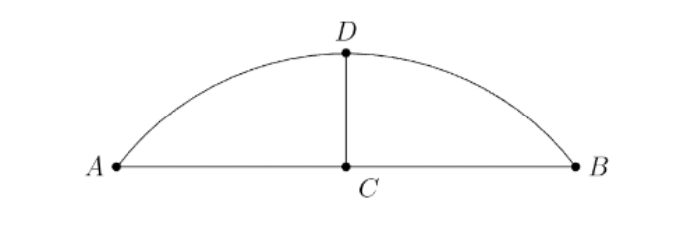
\includegraphics[width=\columnwidth]{olympiad/figs/permo.jpg}
			\caption{}
			\label{fig:plate}
    \end{figure}



    $ C $ is the midpoint of $ AB $, and $ D $ is the midpoint of arc $ AB $. Given that $ AB = 24 $ cm and $ CD = 6 $ cm, what is the radius of the plate in centimeters? (The figure is not drawn to scale.)\hfill(PRMO 2015)
    \item In the coordinate plane, a point is called a lattice point if both of its coordinates are integers. Let $A$ be the point $\brak{12, 84}$. Find the number of right-angled triangles $ABC$ in the coordinate plane where $B$ and $C$ are lattice points, having a right angle at the vertex $A$ and whose incenter is at the origin $\brak{0, 0}$.\hfill(IOQM 2015)
\item Let $ABC$ be an acute-angled triangle with orthocentre $H$, and let $W$ be a point on the side $BC$, lying strictly between $B$ and $C$. The points $M$ and $N$ are the feet of the altitudes from $B$ and $C$ respectively. Denote by $\omega_1$ the circumcircle of $BWN$, and let $X$ be the point on $\omega_1$ such that $WX$ is a diameter of $\omega_1$. Analogously, denote by $\omega_2$ the circumcircle of $CWM$ and let $Y$ be the point on $\omega_2$ such that $WY$ is a diameter of $\omega_2$. Prove that $X$, $Y$ and $H$ are collinear. \hfill(IMO  2013)
\item Let $ABC$ be an acute-angled triangle with circumcentre $O$. Let $P$ on $BC$ be the foot of the altitude from $A$. Suppose that $\angle BC A\geq \angle ABC+30\degree$. Prove that $\angle CAB+\angle COP < \angle 90\degree$.\hfill(IMO 2001)
\item Let $R$ and $S$ be different points on a circle $\Omega$ such that $RS$ is not a diameter. Let $l$ be the tangent line to $\Omega$ at $R$. Point $T$ is such that $S$ is the midpoint of the line segment $RT$. Point $J$ is chosen on the shorter arc $RS$ of $\Omega$ so that the circumcircle $\Gamma$ of triangle $JST$ intersects $l$ at two distinct points. Let $A$ be the common point of $\Gamma$ and $l$ that is closer to $R$. Line $AJ$ meets $\Omega$ again at $K$. Prove that the line $KT$ is tangent to $\Gamma$.\hfill (IMO  2017)
\end{enumerate}

\subsection{JEE}
\begin{enumerate}[label=\thesubsection.\arabic*,ref=\thesubsection.\theenumi]
   % 
    \item Let $ABCD$ be a unit square. Suppose $M$ and $N$ are points on $BC$ and $CD$, respectively, such that the perimeter of triangle $MCN$ is $2$. Let $O$ be the circumcenter of triangle $MAN$, and $P$ be the circumcenter of triangle $MON$. If $\left(\frac{OP}{OA}\right)^2 = \frac{m}{n}$ for some relatively prime positive integers $m$ and $n$, find the value of $m + n$.\hfill(IOQM 2015)
    
    \item In triangle  $ABC$, point $ A_1 $ lies on side $ BC $ and point $B_1$ lies on side $ AC $. Let  $P$ and $ Q $ be points on segments 
$AA_1$ and $BB_1 $, respectively, such that   $PQ \parallel AB$.
Let
 $P_1$ be a point on line  $PB_1$ such that $B_1$ lies strictly between 
$P$ and $P_1$, and $\angle PP_1C$ = $\angle BAC$. Similarly, let $Q_1$ 
be a point on line $QA_1$ such that $A_1$ lies strictly between $Q$ and 
$Q_1$, and $ \angle CQ_1Q$ = $\angle CBA $.
Prove that points $P, Q, P_1,$ and $Q_1$ are concyclic.
\hfill(IMO 2019)


\item Let $D$ be an interior point of the acute triangle $ABC$ with $AB > AC$ so that $\angle DAB = \angle CAD$. The point $E$ on the segment $AC$ satisfies $\angle ADE=\angle BCD$, the point $F$ on the segment $AB$ satisfies $\angle FDA=\angle DBC$, and the point $X$ on the line $AC$ satisfies $CX=BX$. let $O_{1}$ and $O_{2}$ be the circumcentres of the triangles $ADC$ and $EXD$, respectively. Prove that the lines $BC,EF$ and $O_{1} O_{2}$ are concurrent.
 \hfill(IMO 2021)

\item $ABCD$ is cyclic. The feet of the perpendicular from $D$ to the lines $AB$, $BC$, $CA$ are $P, Q,R $ respectivel$y$. Show that the angle bisectors of $ ABC$ and $CDA$ meet on the line $AC$ iff $RP = RQ$.\hfill(IMO 2003)
%
\item In the convex quadrilateral $ABCD$, the diagonals $AC$ and $BD$ are perpendicular and the opposite sides $AB$ and $DC$ are not parallel. Suppose that the point $P$, where the perpendicular bisectors of $AB$and $DC$ meet, is inside $ABCD$. Prove that $ABCD$ is a cyclic quadrilateral if and only if the triangles $ABP$ and $CDP$ have equal areas.

	\hfill(IMO  1998) 
\item Consider five points $A,B,C,D$ and $E$ such that $ABCD$ is a parallelogram and $BCED$ is a cyclic quadrilateral. Let $l$ be a line passing through $A$. Suppose that $l$ intersts the interior of the segment $DC$ at $F$ and intersects line $BC$ at $G$. Suppose also that $EF=EG=EC$. Prove that $l$ is the bisector of angle $DAB$.\hfill(IMO  2007)
		
\item Let $P$ be a point inside triangle $ABC$ such     that                                         
\begin{align*}                                      
	\angle{APB}-\angle{ACB}=\angle{APC}-\angle{ BC}.
 \end{align*}                                       
Let $D$, $E$ be the incenters of triangles $APB$, $APC$, respectively. Show that $AP$, $BD$, $CE$ meet at a point.\hfill(IMO  1996)
\item Let $ABCDEF$ be a convex hexagon such that $A$ is parallel to $DE$, $BC$ is parallel to $EF$, and $CD$ is parallel to $FA$. Let $R_A$, $R_C$, $R_E$ denote the circumradii of triangles $FAB$, $BCD$, $DEF$, respectively, and let $P$ denote the perimeter of the hexagon. Prove that            \hfill(IMO  1996)
\begin{align*}                                            R_A+R_C+R_E\geq\frac{p}{2}.  
\end{align*}
\item The angle at $A$ is the smallest angle of triangle $ABC$. The point $B$ and $C$ divide the circumcircle of the triangle into two arcs. Let $U$ be an interior point of the arc between $B$ and $C$ which does not contain $A$. The perpendicular bisectors of  $AB$ and $AC$ meet the line $AU$ at $V$ and $W$, respctively. The lines $BV$ and $CW$ meet at $T$. Show that
\hfill(IMO  1997)
 \begin{align*}
AU=TB+TC.
 \end{align*}                                   
\item Let $P=A_1A_2 \dots A_k$ be a convex polygon in the plane. The vertices $A_1, A_2,\dots A_k $ have integral coordinates and lie on a circle. Let $S$ be the area of $P$. An odd positive integer $n$ is given such that the squares of the side lengths of $P$ are integers divisible by $n$. Prove that $2S$ is an integer divisible by $n$.\hfill(IMO  2016)
\item Let $I$ be the circumcircle of acute-angled triangle $ABC$. Points $D$ and $E$     lie on segments $AB$ and $AC$ respectively, such that $AD=AE$. The perpendicular bisectors of $BD$ and $CE$ intersect the minor arcs $AB$ and $AC$ of $I$ at points $F$ and $G$ respectively. Prove that the lines $DE$ and $FG$ are parallel (or are the same line).\hfill (IMO  2018)
\item In the plane let $C$ be a circle, $L$ a line  tangent to the circle $C$, and $M$ a point on $L$. Find the locus of all points $P$ with the following property: there exists two points $Q,R$ on $L$ such that $M$ is the midpoint of $QR$ and $C$ is the inscribed circle of triangle $PQR$.  \hfill(IMO  1992)
\item Let $D$ be a point inside acute triangle $ABC$ such that $\angle ADB$ $=$ $\angle ACB$ $+$ $\pi/2$ and $AC \cdot BD = AD \cdot BC$.
 
\begin{enumerate}
\item Calculate the ratio $(AB \cdot CD) / (AC \cdot B)$.
\item Prove that the tangents at $C$ to the circumcircles of $\triangle ACD$ and $\triangle BCD$ are perpendicular. \hfill(IMO  1993)
\end{enumerate}
\item In a triangle $ABC$, let $I$ denote the incenter. Let the lines $AI$, $BI$, and $CI$ intersect the incircle at $P$, $Q$, and $R$, respectively. If $\angle BAC = 40\degree$, what is the value of $\angle QPR$ in degrees?\hfill(PRMO 2014)
\item $AB$ is tangent to the circles $CAMN$ and $NMBD$. $M$ lies between $C$ and $D$ on the line $CD$, and $CD$ is parallel to $AB$. The chords $NA$ and $CM$ meet at $P$; the chords $NB$ and $MD$ meet at $Q$. The rays $CA$ and $DB$ meet at $E$. Prove that $PE = QE$.

	\hfill(IMO 2000)
\item $O$ and $I$ are the circumcentre and incentre of $\triangle ABC$ respectively. Suppose $O$ lies in the interior of $\triangle ABC$ and $I$ lies on the circle passing through $B$, $O$, and $C$. What is the magnitude of $\angle BAC$ in degrees?\hfill(PRMO 2012)
    \item In rectangle $ ABCD $, $ AB = 8 $ and $ BC = 20 $. Let $ P $ be a point on $ AD $ such that $ \angle BPC = 90\degree $. If $ r_1, r_2, r_3 $ are the radii of the incircles of triangles $ APB, BPC $, and $ CPD $, what is the value of $ r_1 + r_2 + r_3 $? \hfill(PRMO 2015)
\item The circle $ \omega $ touches the circle $ \Omega $ internally at $ P $. The center $ O $ of $ \Omega $ is outside $ \omega $. Let $XY$ be a diameter of $ \Omega $ which is also tangent to $ \omega $. Assume $ PY > PX $. Let $ PY $ intersect $ \omega $ at $ Z $. If $ YZ = 2PZ $, what is the magnitude of $ \angle LPYX $ in degrees? 

	\hfill(PRMO 2015)
\item
 Let $I$ be the incentre of acute triangle $ABC$ with $AB$ $\neq AC$. 
The incircle $\omega$ of $ABC$ is tangent to sides $ BC$, $CA$, and $AB$
 at points $D$,  $E$, and $F$, respectively. 
The line 
through $D$ perpendicular to $EF$ meets $\omega$ again at $R$. Line $AR$
 meets $\omega$ again at $P$. The circumcircles of triangles $PCE$ and 
$PBF$ meet again at $Q$.
Prove that lines $DI$ and $PQ$ meet on the line through $ A$ that is perpendicular to $AI$.
\hfill(IMO 2019)
\item Let $r$ be a circle with centre $I$, and $ABCD$ a convex quadrilateral such that each of the segments $AB,BC,CD$ and $DA$ is a tangent to $r$. Let $\Omega$ be the circumcircle of the triangle $AIC$. The extension of $BA$ beyond $A$ meets $\Omega$ at $X$, and the extension of $BC$ beyond $C$ meets $\Omega$ at $Z$. The extensions of $AD$ and $CD$ beyond $D$ meet $\Omega$ at $Y$ and $T$, respectively. Prove that
\begin{align*}
    AD+DT+TX+XA=CD+DY+YZ+ZC
\end{align*}
 \hfill(IMO 2021)
 \item
Let $ABCDE$  be a convex pentagon such that  $BC = DE$.  Assume that there is a point  $T$  inside  $ABCDE$ with  $TB = TD$,  $TC = TE$  and  $\angle{ABT} = \angle{TEA}$.  Let line  $AB$  intersect 
lines $CD$  and  $CT$  at points  $P$  and $Q$,  respectively. Assume that the points  $P, B, A, Q$  occur on their line in that order. Let line  $AE$  intersect lines  $CD$  and  $DT$  at points  $R$  and  $S$,  respectively. Assume 
that the points $ R, E, A, S $ occur on their line in that order. Prove that the points $ P, S, Q, R $ lie on a circle. \hfill(IM0 2022)
\item
Let  $ABC$ be an acute-angled triangle with  $AB \leq AC$. Let $\Omega$  be the circumcircle of  $ABC$.  Let  $S$ be the midpoint of the arc  $CB$  of  $\Omega$ containing $A$.  The perpendicular from $A$  to  $BC$ meets  $BS$  at  $D$  and meets  $\Omega$  again at$ E \neq A$. The line through $
D$ parallel to  $BC$  meets line  $BE$ at  $L$.  Denote the circumcircle of triangle  $BDL$  by  $\omega$.  Let  $\omega$  meet  $\Omega$  again at  $P \neq B$. Prove that the line tangent to $\omega$ at  $P$  meets line $BS$  on the internal angle bisector of  $\angle{BAC}$. \hfill(IMO 2023)
\item
Let  $ABC$  be an equilateral triangle. Let $A_{1}, B_{1}, C_{1}$  be interior points of  $ABC$  such that $ BA_{1} = A_{1}C, CB_{1} = B_{1}A, AC_{1} = C_{1}B,$  and $\angle{BAC} + \angle{CB_{1}A} + \angle{AC_{1}B} = 480^{\circ}.$  Let $ BC_{1}$ and $CB_{1}$  meet at $A_{2}$,  let  $CA_{1}$ and  $A
C_{1}$  meet at  $B_{2}$,  and let  $AB_{1}$ and  $BA_{1}$  meet at  $C_{2}$. Prove that if triangle  $A_{1}B_{1}C_{1}$  is scalene, then the three circumcircles of triangles $AA_{1}A_{2}, BB_{1}B_{2}$  and  $CC_{1}C_{2}$ all pass through two common points.
$\brak{\text{Note: no 2 sides have equal length.}}$ \hfill(IMO 2023)
\item
Let  $ABC$  be a triangle with $ AB \leq AC \leq BC $.  Let the incentre and incircle of triangle   $ABC$  be  $I$ and  $\omega$, respectively. Let $X$ be the point on line  $BC$  different from  $C$  such that the line   through  $X$  parallel to  $AC$  is tangent to  $\omega$.  Similarly, let  $
Y$ be the point on line  $BC$  different from  $B$  such that the line through  $Y$ parallel to  $AB$  is tangent to  $\omega$.  Let $AI$  intersect the circumcircle of  triangle $ABC$  again at  $P \neq A$. Let  $K$  and $L$  be the midpoints of  $AC$  and  $AB$,  respectively.  Prove that  $\angle{KIL} + \angle{YPX} = 180^{\circ}.$ 

\hfill(IMO 2024)
\item In a triangle $ ABC $, let $ H $, $ I $, and $ O $ be the orthocenter, incenter, and circumcenter, respectively. If the points $ B $, $ H $, $ I $, and $ C $ lie on a circle, what is the magnitude of $ \angle BOC $ in degrees?\hfill(PRMO 2013)
\item Let $ S $ be a circle with center $ O $. A chord $ AB $, not a diameter, divides $ S $ into two regions $ R_1 $ and $ R_2 $. Let $ S_1 $ be a circle with center in $ R_1 $ touching $ AB $, the circle $ S $ internally. Let $ S_2 $ be a circle with center in $ R_2 $ touching $ AB $ at $ Y $, the circle $ S $ internally, and passing through the center of $ S $. The point $ X $ lies on the diameter passing through the center of $ S_2 $, and $ \angle YXO = 30\degree $. If the radius of $ S_2 $ is 100, then what is the radius of $ S $?\hfill(PRMO 2013)
\item $BC$ is a diameter of a circle with center $O$. $A$ is any point on the circle with $\angle AOC > 60\degree$. $EF$ is the chord which is the perpendicular bisector of $AO$. $D$ is the midpoint of the minor arc $AB$. The line through $O$ parallel to $AD$ meets $AC$ at $J$. Show that $J$ is the incenter of triangle $CEF$.\hfill(IMO 2002)
\item Let $ABCD$ be a convex quadrilateral such that the line $CD$ is a  tangent to the circle on $AB$ as diameter. Prove that the line $AB$ is a tangent to the  circle on $CD$ as diameter if and only if the lines $BC$ and $AD$ are parallel.\hfill(IMO 1984)
\item let $A$ be one of the two distinct points of intersection of two unequal coplanar tangents to the circles $C_1$ and $C_2$ with centers $ O_1$ and $O_2$, respectively. One of the common tangents to the circles touches $C_1$ at $P_1$ and $C_2$ at $P_2$, while the other touches $C_1$ at $Q_1$ and $C_2$ at $Q_2$.  Let $M_1$ be the midpoint of $P_1Q_1$, $M_2$ be the midpoint of $P_2Q_2$. Prove that $\angle O_1AO_2 =\angle M_1AM_2$.\hfill(IMO 1983)
     \item $A$ circle has center on the side $AB$ of the cyclic quadrilateral $ABCD$. The other three sides are tangent to the circle. Prove that $AD+BC = AB$.\hfill(IMO 1985)
\item A circle with center $O$ passes through the vertices $A$ and $C$ of triangle $ABC$ and intersects the segments $AB$ and $BC$ again at distinct points $K$ and $N$ respectively. The circumscribed circle of the triangle $ABC$ and $EBN$ intersect at exactly two distinct points $B$ and $M$. Prove that angle $OMB$ is a right angle.\hfill(IMO 1985)
\item Three congruent circles have a common point $O$ and lie inside     a given triangle. Each circle touches a pair of sides of the triangle. Prove that the incenter and the circumcenter of the triangle and   the point $O$  are collinear. \hfill(IMO  1981)     
\item A non-isosceles triangle $A_1 A_2 A_3$ is given with sides $a_1,a_2,a_3$ ($a_i$ is the side opposite $A_i$). For all $i = 1, 2, 3, M_i$ is the midpoint of side $a_i$ and $T_i$ is the point where     the incircle touches side $a_i$. Denote by $S_i$ the reflection of $T_i$ in the interior bisector of angle $A_i$. Prove that the lines $M_1S_1$, $ M_2S_2$ and $M_3S_3$ are concurrent.\hfill(IMO  1982)
    \item In an acute-angled triangle $ABC$ the interior bisector of the angle $A$ intersects $BC$ at $L$ and intersects the circumcircle of $ABC$ again at $N$. From point $L$ perpendiculars are drawn to $AB$ and $AC$, the feet of these perpendiculars being $K$ and $M$ respectively. Prove that the quadrilateral $AKNM$ and the triangle $ABC$ have equal areas.

	    \hfill(IMO  1987)
    \item Consider two coplanar circles of radii $R$ and $r$ $\brak{R > r}$ with the same center. Let $P$ be a fixed point on the smaller circle and $B$ a variable point on the larger circle. The line $BP$ meets the larger circle again at $C$. The perpendicular $l$ to $BP $ at $P$ meets the smaller circle again at $A$. (If $l$ is tangent to the circle at $P$ then $A = P$).
\hfill(IMO  1988)
\begin{enumerate}
	\item  Find the set of values of $BC^2+CA^2+AB^2$ 
	\item  Find the locus of the midpoint of $BC$.
\end{enumerate}
\item  Let the excircle of triangle $ABC$ opposite the vertex $A$ be tangent to the side $BC$ at the point $A_1$. Define the points $B_1$ on $CA$ and $C_1$ on $AB$ analogously, using the excircles opposite $B$ and $C$ respectively. Suppose that the circumcentre of triangle $A_1B_1C_1$, lies on the circumcircle of triangle $ABC$. Prove that triangle $ABC$ is right-angled. 
	(The excircle of triangle $ABC$ opposite the vertex $A$ is the circle that is tangent to the line segment $BC$, to the ray $AB$ beyond $B$, and to the ray $AC$ beyond $C$. The excircles opposite $B$ and $C$ are similarly defined. \hfill(IMO  2013)
\item  Convex quadrilateral $ABCD$ has $\angle ABC= \angle CDA = 90 \degree$. Point $H$ is the foot of the perpendicular from $A$ to $BD$. Points $S$ and $T$ lie on sides $AB$ and $AD$ respectively, such that $H$ lies inside triangle $SCT$ and $\angle CHS- \angle CSB = 90 \degree, \angle THC- \angle DTC = 90\degree$.
	Prove that line $BD$ is tangent to the circumcircle of triangle $TSH$.
	\hfill(IMO  2014)
\item   Points $P$ and $Q$ lie on side $BC$ of acute-angled triangle $ABC$ so that $\angle PAB= \angle BCA$ and $\angle CAQ=\angle ABC.$ Points $M$ and $N$ lie on lines $AP$ and $AQ,$ respectively, such that $P$ is the midpoint of $AM,$ and $Q$ is the midpoint of $AN.$ Prove that lines $BM$ and $CN$ intersect on circumcircle of triangle $ABC$ \hfill(IMO  2014)
\item   Let $ABC$ be an acute triangle with $AB > AC$. Let $I$ be its circumcircle, $H$ its orthocentre, and $F$ the foot of the altitude from $A$. Let $M$ be the midpoint of $BC$. Let $Q$ be the point on $T$ such that $\angle HQA= 90$, and let $K$ be the point on $T$ such that $\angle HKQ=90\degree.$ Assume that the points $ A, B, C, K$ and $Q$ are all different, and lie on $T$ in this order.
	Prove that the circumcircles of triangles $KQH$ and $FKM$ are tangent to each other. \hfill(IMO 2015)
\item  Triangle $ABC$ has circumcircle $\Omega$ and circumcentre $O$. A circle $T$ with centre $A$ intersects the segment $BC$ at points $D$ and $E$, such that $B, D, E $ and $C$ are all different and lie on line $BC$ in this order. Let $F$ and $G$ be the points of intersection of $T$ and $\Omega$ such that $A, F, B, C$ and $G$ lie on $\Omega$ in this order. Let $K $ be the second point of intersection of the circumcircle of triangle $BDF$ and the segment $AB$. Let $L$ be the second point of intersection of the circumcircle of triangle $CGE$ and the segment $CA$.
	Suppose that the lines $FK$ and $GL$ are different and intersect at the point $X$. Prove that $X$ lies on the line $AO$. \hfill(IMO  2015)
\item In an acute-angled triangle $ABC$, the internal bisector of angle $A$ meets the circumcircle of the triangle again at $A_1$. Points $B_1$ and $C_1$ are defined similarly. Let $A_0$ be the point of intersection of the line $AA_1$ with the external bisectors of angles $B$ and $C$. Points $B_0$ and $C_0$ are defined similarly. Prove that
\begin{enumerate}
\item The area of the triangle $A_0$ $B_0C_0$ is twice the area of the hexagon $AC_1BA_1CB_1$
\item  The area of the triangle $A_0B_0C_0$ is at least four times the area of the triangle $ABC$. 

	\hfill(IMO  1989)
\end{enumerate}
   \item Chords $AB$ and $CD$ of a circle intersect at a point $E$ inside the circle. Let $M$ be an interior point of the segment $EB$. The tangent line at $E$ to the circle through $D, E$ and $M$ intersects the lines $BC$ and $AC$ at $F$ and $G$ respectively. If $\frac{AM}{AB}=t$,
  find $ \frac{EG}{EF}$  
	  in terms of $t$.\hfill(IMO  1990)
\item In triangle $ABC$, $AB = AC$. A circle is tangent internally to the circumcircle of triangle $ABC$ and also to sides $AB, AC$ at $P, Q$, respectively. Prove that the midpoint of segment $PQ$ is the center of the incircle of triangle $ABC.$\hfill(IMO  1978)
\item Two circles in a plane intersect. Let $A$ be one of the points of intersection. Starting simultaneously from $A$ two points move with constant speeds, each point travelling along its own circle in the same sense. The two points return to $A$ simultaneously after one revolution. Prove that there is a fixed point $P$ in the plane such that, at any time, the distances from $P$ to the moving points are equal.\hfill(IMO  1979) 
\item Let $I$ be the incenter of triangle $ABC$. Let the incircle of $ABC$ touch the sides $BC$,$CA$, and $AB$ at $K$, $L$, and $M$, respectively. The line through $B$ parallel to $MK$ meets the lines $LM$ and $LK$ at $R$ and $S$ respectively. Prove that angle $RIS$ is acute.\hfill(IMO  1998)
%
\item Two circles ${G_{1}}$ and ${G_{2}}$ are contained inside the circle $G$, and are tangent to $G$ at the distinct points $M$ and $N$, respectively. ${G_{1}}$ passes through the center of ${G_{2}}$. The line passing through the two points of intersection of ${G_{1}}$ and ${G_{2}}$ meets $G$ at $A$ and $B$. The lines $MA$ and $MB$ meet ${G_{1}}$ at $C$ and $D$ respectively. Prove that $CD$ is tangent to ${G_{2}}$.\hfill(IMO  1999)
                      	
\item ${A_{1}} {A_{2}} {A_{3}}$ is an acute-angled triangle. The foot of the altitude from ${A_{i}}$ is ${K_{i}}$ and the incircle touches the side opposite ${A_{i}}$ at ${L_{i}}$. The line ${K_{1}}{K_{2}}$ is reflected in the line ${L_{1}}{L_{2}}$. Similarly, the line ${K_{2}}{K_{3}}$ is reflected in ${L_{2}}{L_{3}}$ and ${K_{3}}{K_{1}}$ is reflected in ${L_{3}}{L_{1}}$. Show that the three new lines form a triangle with vertices on the incircle.\hfill(IMO  2000)
\item Let $ABC$ be an acute-angled triangle  with $AB$ $\neq$ $AC$. The circle with diameter $BC$ intersects the sides $AB$ and $AC$ at $M$ and $N$ respectively. Denote by $O$ the midpoint of the side $BC$. The bisectors of the angles $BAC$ and $MON$ intersect at $R$. Prove that the circumcircles of the triangles $BMR$ and $CNR$ have a common point on the side $BC$. \hfill(IMO  2004)
 \item In a convex quadrilateral $ABCD$ the diagonal $BD$ does not bisect the angles $ABC$ and $CDA$. The point $P$ lies inside $ABCD$ and satisfies
 \begin{align*}
	 \angle{PBC}=\angle{DBA} \text{ and } \angle{PDC}=\angle{BDA}.
 \end{align*}
Prove that $ABCD$ is a cyclic quadrilateral if and only if $AP=CP$. \hfill(IMO  2004)
\item Let $ABCD$ be a fixed convex quadrilateral with $BC$ = $DA$ and
    $BC$ not parallel with $DA$. Let two variable points $E$ and $F$ lie on the sides $BC$ and $DA$, respectively and satisfy $BEDF$. The lines $AC$ and $BD$ meet at $P$, the lines $BD$ and $EF$ meet at $Q$, the lines $EF$ and $AC$ meet at $R$. Prove that the circumcircles of the triangles $PQR$, as $E$ and $F$ vary, have a common point other than $P$.\hfill(IMO  2005)
	\item In triangle $ABC$ the bisector of angle $BCA$ intersects the circumcircle again at $R$, the perpendicular bisector of $BC$ at $P$, and the perpendicular bisector of $AC$ at $Q$. The midpoint of $BC$ is $K$ and the midpoint of $AC$ is $L$. Prove that the triangles $RPK$ and $RQL$ have the same area.\hfill(IMO  2007)
	\item An acute-angled triangle $ABC$ has orthocentre $H$. The circle passing through $H$ with centre the midpoint of $BC$ intersects the line $BC$ at $A_1$ and $A_2$. Similarly, the circle passing through $H$ with centre the midpoint of $CA$ intersects the line $CA$ at $B_1$ and $B_2$, and the circle passing through $H$ with centre the midpoint of $AB$ intersects the line $AB$ at $C_1$ and $C_2$. Show that $A_1$, $A_2$, $B_1$, $B_2$, $C_1$, $C_2$ lie on a circle.\hfill(IMO  2008)
	\item Let $ABCD$ be a convex quadrilateral with $|BA| \neq |BC|$. Denote the incircles of triangles $ABC$ and $ADC$ by $\omega_{1}$ and $\omega_{2}$ respectively. Suppose that there exists a circle $\omega$ tangent to the ray $BA$ beyond $A$ and to the ray $BC$ beyond $C$, which is also tangent to the lines $AD$ and $CD$. Prove that the common external tangents of $\omega_{1}$ and $\omega_{2}$ intersect on $\omega$.\hfill(IMO  2008)
		\item Let $ABC$ be a triangle with circumcentre $O$. The points $P$  and $Q$ are interior points of the sides $CA$ and $AB$, respectively. Let $K,L$ and $M$ be the midpoints of the segments $BP$, $CQ$ and $PQ$, respectively, and let $\Gamma$ be the circle passing through $K,L$ and $M$. Suppose that the line $PQ$ is tangent to the circle $\Gamma$. Prove that $OP=OQ$.

			\hfill(IMO  2009)
	\item Let $ABC$ be a triangle with $AB=AC$. The angle bisectors of $\angle CAB$ and $\angle ABC$ meet the sides $BC$ and $CA$ at $D$ and $E$, respectively. Let $K$ be the incentre of triangle $ADC$. Suppose that $ \angle BEK$=$45\degree$. Find all possible values of $\angle CAB$.\hfill(IMO  2009)
	\item Let $A$,$B$,$C$,$D$ be four distinct points on a line, in that order. The circles with diameters $AC$ and $BD$ intersect at $X$ and $Y$. The line $XY$ meets $BC$ at $Z$. Let $P$ be a point on the line $XY$ other than $Z$. The line $CP$ intersects the circle with diameter $AC$ at $C$ and $M$, and the line $BP$ intersects the circle with diameter $BD$ at $B$ and $N$. Prove that the lines $AM$, $DN$, $XY$ are concurrent.\hfill(IMO  1995)
\item $PS$ is a line segment of length 4 and $O$ is the midpoint of $PS$. A semicircular arc is drawn with $PS$ as diameter. Let $X$ be the midpoint of this arc. $Q$ and $R$ are points on the arc $PXS$ such that $QR$ is parallel to $PS$ and the semicircular arc drawn with $QR$ as diameter is tangent to $PS$. What is the area of the region $QXROQ$ bounded by the two semicircular arcs?\hfill(PRMO 2012)
\item The figure below shows a broken piece of a circular plate made of glass.
		\begin{figure}[h!]
    \centering
	    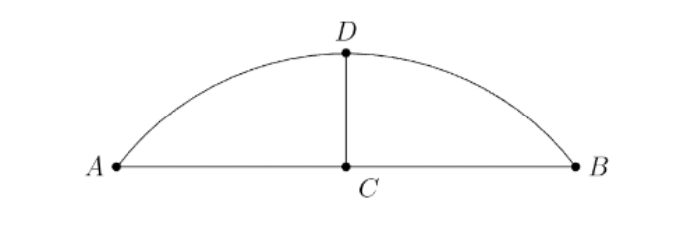
\includegraphics[width=\columnwidth]{olympiad/figs/permo.jpg}
			\caption{}
			\label{fig:plate}
    \end{figure}



    $ C $ is the midpoint of $ AB $, and $ D $ is the midpoint of arc $ AB $. Given that $ AB = 24 $ cm and $ CD = 6 $ cm, what is the radius of the plate in centimeters? (The figure is not drawn to scale.)\hfill(PRMO 2015)
    \item In the coordinate plane, a point is called a lattice point if both of its coordinates are integers. Let $A$ be the point $\brak{12, 84}$. Find the number of right-angled triangles $ABC$ in the coordinate plane where $B$ and $C$ are lattice points, having a right angle at the vertex $A$ and whose incenter is at the origin $\brak{0, 0}$.\hfill(IOQM 2015)
\item Let $ABC$ be an acute-angled triangle with orthocentre $H$, and let $W$ be a point on the side $BC$, lying strictly between $B$ and $C$. The points $M$ and $N$ are the feet of the altitudes from $B$ and $C$ respectively. Denote by $\omega_1$ the circumcircle of $BWN$, and let $X$ be the point on $\omega_1$ such that $WX$ is a diameter of $\omega_1$. Analogously, denote by $\omega_2$ the circumcircle of $CWM$ and let $Y$ be the point on $\omega_2$ such that $WY$ is a diameter of $\omega_2$. Prove that $X$, $Y$ and $H$ are collinear. \hfill(IMO  2013)
\item Let $ABC$ be an acute-angled triangle with circumcentre $O$. Let $P$ on $BC$ be the foot of the altitude from $A$. Suppose that $\angle BC A\geq \angle ABC+30\degree$. Prove that $\angle CAB+\angle COP < \angle 90\degree$.\hfill(IMO 2001)
\item Let $R$ and $S$ be different points on a circle $\Omega$ such that $RS$ is not a diameter. Let $l$ be the tangent line to $\Omega$ at $R$. Point $T$ is such that $S$ is the midpoint of the line segment $RT$. Point $J$ is chosen on the shorter arc $RS$ of $\Omega$ so that the circumcircle $\Gamma$ of triangle $JST$ intersects $l$ at two distinct points. Let $A$ be the common point of $\Gamma$ and $l$ that is closer to $R$. Line $AJ$ meets $\Omega$ again at $K$. Prove that the line $KT$ is tangent to $\Gamma$.\hfill (IMO  2017)
\end{enumerate}

\subsection{Olympiad}
\begin{enumerate}[label=\thesubsection.\arabic*,ref=\thesubsection.\theenumi]
   % 
    \item Let $ABCD$ be a unit square. Suppose $M$ and $N$ are points on $BC$ and $CD$, respectively, such that the perimeter of triangle $MCN$ is $2$. Let $O$ be the circumcenter of triangle $MAN$, and $P$ be the circumcenter of triangle $MON$. If $\left(\frac{OP}{OA}\right)^2 = \frac{m}{n}$ for some relatively prime positive integers $m$ and $n$, find the value of $m + n$.\hfill(IOQM 2015)
    
    \item In triangle  $ABC$, point $ A_1 $ lies on side $ BC $ and point $B_1$ lies on side $ AC $. Let  $P$ and $ Q $ be points on segments 
$AA_1$ and $BB_1 $, respectively, such that   $PQ \parallel AB$.
Let
 $P_1$ be a point on line  $PB_1$ such that $B_1$ lies strictly between 
$P$ and $P_1$, and $\angle PP_1C$ = $\angle BAC$. Similarly, let $Q_1$ 
be a point on line $QA_1$ such that $A_1$ lies strictly between $Q$ and 
$Q_1$, and $ \angle CQ_1Q$ = $\angle CBA $.
Prove that points $P, Q, P_1,$ and $Q_1$ are concyclic.
\hfill(IMO 2019)


\item Let $D$ be an interior point of the acute triangle $ABC$ with $AB > AC$ so that $\angle DAB = \angle CAD$. The point $E$ on the segment $AC$ satisfies $\angle ADE=\angle BCD$, the point $F$ on the segment $AB$ satisfies $\angle FDA=\angle DBC$, and the point $X$ on the line $AC$ satisfies $CX=BX$. let $O_{1}$ and $O_{2}$ be the circumcentres of the triangles $ADC$ and $EXD$, respectively. Prove that the lines $BC,EF$ and $O_{1} O_{2}$ are concurrent.
 \hfill(IMO 2021)

\item $ABCD$ is cyclic. The feet of the perpendicular from $D$ to the lines $AB$, $BC$, $CA$ are $P, Q,R $ respectivel$y$. Show that the angle bisectors of $ ABC$ and $CDA$ meet on the line $AC$ iff $RP = RQ$.\hfill(IMO 2003)
%
\item In the convex quadrilateral $ABCD$, the diagonals $AC$ and $BD$ are perpendicular and the opposite sides $AB$ and $DC$ are not parallel. Suppose that the point $P$, where the perpendicular bisectors of $AB$and $DC$ meet, is inside $ABCD$. Prove that $ABCD$ is a cyclic quadrilateral if and only if the triangles $ABP$ and $CDP$ have equal areas.

	\hfill(IMO  1998) 
\item Consider five points $A,B,C,D$ and $E$ such that $ABCD$ is a parallelogram and $BCED$ is a cyclic quadrilateral. Let $l$ be a line passing through $A$. Suppose that $l$ intersts the interior of the segment $DC$ at $F$ and intersects line $BC$ at $G$. Suppose also that $EF=EG=EC$. Prove that $l$ is the bisector of angle $DAB$.\hfill(IMO  2007)
		
\item Let $P$ be a point inside triangle $ABC$ such     that                                         
\begin{align*}                                      
	\angle{APB}-\angle{ACB}=\angle{APC}-\angle{ BC}.
 \end{align*}                                       
Let $D$, $E$ be the incenters of triangles $APB$, $APC$, respectively. Show that $AP$, $BD$, $CE$ meet at a point.\hfill(IMO  1996)
\item Let $ABCDEF$ be a convex hexagon such that $A$ is parallel to $DE$, $BC$ is parallel to $EF$, and $CD$ is parallel to $FA$. Let $R_A$, $R_C$, $R_E$ denote the circumradii of triangles $FAB$, $BCD$, $DEF$, respectively, and let $P$ denote the perimeter of the hexagon. Prove that            \hfill(IMO  1996)
\begin{align*}                                            R_A+R_C+R_E\geq\frac{p}{2}.  
\end{align*}
\item The angle at $A$ is the smallest angle of triangle $ABC$. The point $B$ and $C$ divide the circumcircle of the triangle into two arcs. Let $U$ be an interior point of the arc between $B$ and $C$ which does not contain $A$. The perpendicular bisectors of  $AB$ and $AC$ meet the line $AU$ at $V$ and $W$, respctively. The lines $BV$ and $CW$ meet at $T$. Show that
\hfill(IMO  1997)
 \begin{align*}
AU=TB+TC.
 \end{align*}                                   
\item Let $P=A_1A_2 \dots A_k$ be a convex polygon in the plane. The vertices $A_1, A_2,\dots A_k $ have integral coordinates and lie on a circle. Let $S$ be the area of $P$. An odd positive integer $n$ is given such that the squares of the side lengths of $P$ are integers divisible by $n$. Prove that $2S$ is an integer divisible by $n$.\hfill(IMO  2016)
\item Let $I$ be the circumcircle of acute-angled triangle $ABC$. Points $D$ and $E$     lie on segments $AB$ and $AC$ respectively, such that $AD=AE$. The perpendicular bisectors of $BD$ and $CE$ intersect the minor arcs $AB$ and $AC$ of $I$ at points $F$ and $G$ respectively. Prove that the lines $DE$ and $FG$ are parallel (or are the same line).\hfill (IMO  2018)
\item In the plane let $C$ be a circle, $L$ a line  tangent to the circle $C$, and $M$ a point on $L$. Find the locus of all points $P$ with the following property: there exists two points $Q,R$ on $L$ such that $M$ is the midpoint of $QR$ and $C$ is the inscribed circle of triangle $PQR$.  \hfill(IMO  1992)
\item Let $D$ be a point inside acute triangle $ABC$ such that $\angle ADB$ $=$ $\angle ACB$ $+$ $\pi/2$ and $AC \cdot BD = AD \cdot BC$.
 
\begin{enumerate}
\item Calculate the ratio $(AB \cdot CD) / (AC \cdot B)$.
\item Prove that the tangents at $C$ to the circumcircles of $\triangle ACD$ and $\triangle BCD$ are perpendicular. \hfill(IMO  1993)
\end{enumerate}
\item In a triangle $ABC$, let $I$ denote the incenter. Let the lines $AI$, $BI$, and $CI$ intersect the incircle at $P$, $Q$, and $R$, respectively. If $\angle BAC = 40\degree$, what is the value of $\angle QPR$ in degrees?\hfill(PRMO 2014)
\item $AB$ is tangent to the circles $CAMN$ and $NMBD$. $M$ lies between $C$ and $D$ on the line $CD$, and $CD$ is parallel to $AB$. The chords $NA$ and $CM$ meet at $P$; the chords $NB$ and $MD$ meet at $Q$. The rays $CA$ and $DB$ meet at $E$. Prove that $PE = QE$.

	\hfill(IMO 2000)
\item $O$ and $I$ are the circumcentre and incentre of $\triangle ABC$ respectively. Suppose $O$ lies in the interior of $\triangle ABC$ and $I$ lies on the circle passing through $B$, $O$, and $C$. What is the magnitude of $\angle BAC$ in degrees?\hfill(PRMO 2012)
    \item In rectangle $ ABCD $, $ AB = 8 $ and $ BC = 20 $. Let $ P $ be a point on $ AD $ such that $ \angle BPC = 90\degree $. If $ r_1, r_2, r_3 $ are the radii of the incircles of triangles $ APB, BPC $, and $ CPD $, what is the value of $ r_1 + r_2 + r_3 $? \hfill(PRMO 2015)
\item The circle $ \omega $ touches the circle $ \Omega $ internally at $ P $. The center $ O $ of $ \Omega $ is outside $ \omega $. Let $XY$ be a diameter of $ \Omega $ which is also tangent to $ \omega $. Assume $ PY > PX $. Let $ PY $ intersect $ \omega $ at $ Z $. If $ YZ = 2PZ $, what is the magnitude of $ \angle LPYX $ in degrees? 

	\hfill(PRMO 2015)
\item
 Let $I$ be the incentre of acute triangle $ABC$ with $AB$ $\neq AC$. 
The incircle $\omega$ of $ABC$ is tangent to sides $ BC$, $CA$, and $AB$
 at points $D$,  $E$, and $F$, respectively. 
The line 
through $D$ perpendicular to $EF$ meets $\omega$ again at $R$. Line $AR$
 meets $\omega$ again at $P$. The circumcircles of triangles $PCE$ and 
$PBF$ meet again at $Q$.
Prove that lines $DI$ and $PQ$ meet on the line through $ A$ that is perpendicular to $AI$.
\hfill(IMO 2019)
\item Let $r$ be a circle with centre $I$, and $ABCD$ a convex quadrilateral such that each of the segments $AB,BC,CD$ and $DA$ is a tangent to $r$. Let $\Omega$ be the circumcircle of the triangle $AIC$. The extension of $BA$ beyond $A$ meets $\Omega$ at $X$, and the extension of $BC$ beyond $C$ meets $\Omega$ at $Z$. The extensions of $AD$ and $CD$ beyond $D$ meet $\Omega$ at $Y$ and $T$, respectively. Prove that
\begin{align*}
    AD+DT+TX+XA=CD+DY+YZ+ZC
\end{align*}
 \hfill(IMO 2021)
 \item
Let $ABCDE$  be a convex pentagon such that  $BC = DE$.  Assume that there is a point  $T$  inside  $ABCDE$ with  $TB = TD$,  $TC = TE$  and  $\angle{ABT} = \angle{TEA}$.  Let line  $AB$  intersect 
lines $CD$  and  $CT$  at points  $P$  and $Q$,  respectively. Assume that the points  $P, B, A, Q$  occur on their line in that order. Let line  $AE$  intersect lines  $CD$  and  $DT$  at points  $R$  and  $S$,  respectively. Assume 
that the points $ R, E, A, S $ occur on their line in that order. Prove that the points $ P, S, Q, R $ lie on a circle. \hfill(IM0 2022)
\item
Let  $ABC$ be an acute-angled triangle with  $AB \leq AC$. Let $\Omega$  be the circumcircle of  $ABC$.  Let  $S$ be the midpoint of the arc  $CB$  of  $\Omega$ containing $A$.  The perpendicular from $A$  to  $BC$ meets  $BS$  at  $D$  and meets  $\Omega$  again at$ E \neq A$. The line through $
D$ parallel to  $BC$  meets line  $BE$ at  $L$.  Denote the circumcircle of triangle  $BDL$  by  $\omega$.  Let  $\omega$  meet  $\Omega$  again at  $P \neq B$. Prove that the line tangent to $\omega$ at  $P$  meets line $BS$  on the internal angle bisector of  $\angle{BAC}$. \hfill(IMO 2023)
\item
Let  $ABC$  be an equilateral triangle. Let $A_{1}, B_{1}, C_{1}$  be interior points of  $ABC$  such that $ BA_{1} = A_{1}C, CB_{1} = B_{1}A, AC_{1} = C_{1}B,$  and $\angle{BAC} + \angle{CB_{1}A} + \angle{AC_{1}B} = 480^{\circ}.$  Let $ BC_{1}$ and $CB_{1}$  meet at $A_{2}$,  let  $CA_{1}$ and  $A
C_{1}$  meet at  $B_{2}$,  and let  $AB_{1}$ and  $BA_{1}$  meet at  $C_{2}$. Prove that if triangle  $A_{1}B_{1}C_{1}$  is scalene, then the three circumcircles of triangles $AA_{1}A_{2}, BB_{1}B_{2}$  and  $CC_{1}C_{2}$ all pass through two common points.
$\brak{\text{Note: no 2 sides have equal length.}}$ \hfill(IMO 2023)
\item
Let  $ABC$  be a triangle with $ AB \leq AC \leq BC $.  Let the incentre and incircle of triangle   $ABC$  be  $I$ and  $\omega$, respectively. Let $X$ be the point on line  $BC$  different from  $C$  such that the line   through  $X$  parallel to  $AC$  is tangent to  $\omega$.  Similarly, let  $
Y$ be the point on line  $BC$  different from  $B$  such that the line through  $Y$ parallel to  $AB$  is tangent to  $\omega$.  Let $AI$  intersect the circumcircle of  triangle $ABC$  again at  $P \neq A$. Let  $K$  and $L$  be the midpoints of  $AC$  and  $AB$,  respectively.  Prove that  $\angle{KIL} + \angle{YPX} = 180^{\circ}.$ 

\hfill(IMO 2024)
\item In a triangle $ ABC $, let $ H $, $ I $, and $ O $ be the orthocenter, incenter, and circumcenter, respectively. If the points $ B $, $ H $, $ I $, and $ C $ lie on a circle, what is the magnitude of $ \angle BOC $ in degrees?\hfill(PRMO 2013)
\item Let $ S $ be a circle with center $ O $. A chord $ AB $, not a diameter, divides $ S $ into two regions $ R_1 $ and $ R_2 $. Let $ S_1 $ be a circle with center in $ R_1 $ touching $ AB $, the circle $ S $ internally. Let $ S_2 $ be a circle with center in $ R_2 $ touching $ AB $ at $ Y $, the circle $ S $ internally, and passing through the center of $ S $. The point $ X $ lies on the diameter passing through the center of $ S_2 $, and $ \angle YXO = 30\degree $. If the radius of $ S_2 $ is 100, then what is the radius of $ S $?\hfill(PRMO 2013)
\item $BC$ is a diameter of a circle with center $O$. $A$ is any point on the circle with $\angle AOC > 60\degree$. $EF$ is the chord which is the perpendicular bisector of $AO$. $D$ is the midpoint of the minor arc $AB$. The line through $O$ parallel to $AD$ meets $AC$ at $J$. Show that $J$ is the incenter of triangle $CEF$.\hfill(IMO 2002)
\item Let $ABCD$ be a convex quadrilateral such that the line $CD$ is a  tangent to the circle on $AB$ as diameter. Prove that the line $AB$ is a tangent to the  circle on $CD$ as diameter if and only if the lines $BC$ and $AD$ are parallel.\hfill(IMO 1984)
\item let $A$ be one of the two distinct points of intersection of two unequal coplanar tangents to the circles $C_1$ and $C_2$ with centers $ O_1$ and $O_2$, respectively. One of the common tangents to the circles touches $C_1$ at $P_1$ and $C_2$ at $P_2$, while the other touches $C_1$ at $Q_1$ and $C_2$ at $Q_2$.  Let $M_1$ be the midpoint of $P_1Q_1$, $M_2$ be the midpoint of $P_2Q_2$. Prove that $\angle O_1AO_2 =\angle M_1AM_2$.\hfill(IMO 1983)
     \item $A$ circle has center on the side $AB$ of the cyclic quadrilateral $ABCD$. The other three sides are tangent to the circle. Prove that $AD+BC = AB$.\hfill(IMO 1985)
\item A circle with center $O$ passes through the vertices $A$ and $C$ of triangle $ABC$ and intersects the segments $AB$ and $BC$ again at distinct points $K$ and $N$ respectively. The circumscribed circle of the triangle $ABC$ and $EBN$ intersect at exactly two distinct points $B$ and $M$. Prove that angle $OMB$ is a right angle.\hfill(IMO 1985)
\item Three congruent circles have a common point $O$ and lie inside     a given triangle. Each circle touches a pair of sides of the triangle. Prove that the incenter and the circumcenter of the triangle and   the point $O$  are collinear. \hfill(IMO  1981)     
\item A non-isosceles triangle $A_1 A_2 A_3$ is given with sides $a_1,a_2,a_3$ ($a_i$ is the side opposite $A_i$). For all $i = 1, 2, 3, M_i$ is the midpoint of side $a_i$ and $T_i$ is the point where     the incircle touches side $a_i$. Denote by $S_i$ the reflection of $T_i$ in the interior bisector of angle $A_i$. Prove that the lines $M_1S_1$, $ M_2S_2$ and $M_3S_3$ are concurrent.\hfill(IMO  1982)
    \item In an acute-angled triangle $ABC$ the interior bisector of the angle $A$ intersects $BC$ at $L$ and intersects the circumcircle of $ABC$ again at $N$. From point $L$ perpendiculars are drawn to $AB$ and $AC$, the feet of these perpendiculars being $K$ and $M$ respectively. Prove that the quadrilateral $AKNM$ and the triangle $ABC$ have equal areas.

	    \hfill(IMO  1987)
    \item Consider two coplanar circles of radii $R$ and $r$ $\brak{R > r}$ with the same center. Let $P$ be a fixed point on the smaller circle and $B$ a variable point on the larger circle. The line $BP$ meets the larger circle again at $C$. The perpendicular $l$ to $BP $ at $P$ meets the smaller circle again at $A$. (If $l$ is tangent to the circle at $P$ then $A = P$).
\hfill(IMO  1988)
\begin{enumerate}
	\item  Find the set of values of $BC^2+CA^2+AB^2$ 
	\item  Find the locus of the midpoint of $BC$.
\end{enumerate}
\item  Let the excircle of triangle $ABC$ opposite the vertex $A$ be tangent to the side $BC$ at the point $A_1$. Define the points $B_1$ on $CA$ and $C_1$ on $AB$ analogously, using the excircles opposite $B$ and $C$ respectively. Suppose that the circumcentre of triangle $A_1B_1C_1$, lies on the circumcircle of triangle $ABC$. Prove that triangle $ABC$ is right-angled. 
	(The excircle of triangle $ABC$ opposite the vertex $A$ is the circle that is tangent to the line segment $BC$, to the ray $AB$ beyond $B$, and to the ray $AC$ beyond $C$. The excircles opposite $B$ and $C$ are similarly defined. \hfill(IMO  2013)
\item  Convex quadrilateral $ABCD$ has $\angle ABC= \angle CDA = 90 \degree$. Point $H$ is the foot of the perpendicular from $A$ to $BD$. Points $S$ and $T$ lie on sides $AB$ and $AD$ respectively, such that $H$ lies inside triangle $SCT$ and $\angle CHS- \angle CSB = 90 \degree, \angle THC- \angle DTC = 90\degree$.
	Prove that line $BD$ is tangent to the circumcircle of triangle $TSH$.
	\hfill(IMO  2014)
\item   Points $P$ and $Q$ lie on side $BC$ of acute-angled triangle $ABC$ so that $\angle PAB= \angle BCA$ and $\angle CAQ=\angle ABC.$ Points $M$ and $N$ lie on lines $AP$ and $AQ,$ respectively, such that $P$ is the midpoint of $AM,$ and $Q$ is the midpoint of $AN.$ Prove that lines $BM$ and $CN$ intersect on circumcircle of triangle $ABC$ \hfill(IMO  2014)
\item   Let $ABC$ be an acute triangle with $AB > AC$. Let $I$ be its circumcircle, $H$ its orthocentre, and $F$ the foot of the altitude from $A$. Let $M$ be the midpoint of $BC$. Let $Q$ be the point on $T$ such that $\angle HQA= 90$, and let $K$ be the point on $T$ such that $\angle HKQ=90\degree.$ Assume that the points $ A, B, C, K$ and $Q$ are all different, and lie on $T$ in this order.
	Prove that the circumcircles of triangles $KQH$ and $FKM$ are tangent to each other. \hfill(IMO 2015)
\item  Triangle $ABC$ has circumcircle $\Omega$ and circumcentre $O$. A circle $T$ with centre $A$ intersects the segment $BC$ at points $D$ and $E$, such that $B, D, E $ and $C$ are all different and lie on line $BC$ in this order. Let $F$ and $G$ be the points of intersection of $T$ and $\Omega$ such that $A, F, B, C$ and $G$ lie on $\Omega$ in this order. Let $K $ be the second point of intersection of the circumcircle of triangle $BDF$ and the segment $AB$. Let $L$ be the second point of intersection of the circumcircle of triangle $CGE$ and the segment $CA$.
	Suppose that the lines $FK$ and $GL$ are different and intersect at the point $X$. Prove that $X$ lies on the line $AO$. \hfill(IMO  2015)
\item In an acute-angled triangle $ABC$, the internal bisector of angle $A$ meets the circumcircle of the triangle again at $A_1$. Points $B_1$ and $C_1$ are defined similarly. Let $A_0$ be the point of intersection of the line $AA_1$ with the external bisectors of angles $B$ and $C$. Points $B_0$ and $C_0$ are defined similarly. Prove that
\begin{enumerate}
\item The area of the triangle $A_0$ $B_0C_0$ is twice the area of the hexagon $AC_1BA_1CB_1$
\item  The area of the triangle $A_0B_0C_0$ is at least four times the area of the triangle $ABC$. 

	\hfill(IMO  1989)
\end{enumerate}
   \item Chords $AB$ and $CD$ of a circle intersect at a point $E$ inside the circle. Let $M$ be an interior point of the segment $EB$. The tangent line at $E$ to the circle through $D, E$ and $M$ intersects the lines $BC$ and $AC$ at $F$ and $G$ respectively. If $\frac{AM}{AB}=t$,
  find $ \frac{EG}{EF}$  
	  in terms of $t$.\hfill(IMO  1990)
\item In triangle $ABC$, $AB = AC$. A circle is tangent internally to the circumcircle of triangle $ABC$ and also to sides $AB, AC$ at $P, Q$, respectively. Prove that the midpoint of segment $PQ$ is the center of the incircle of triangle $ABC.$\hfill(IMO  1978)
\item Two circles in a plane intersect. Let $A$ be one of the points of intersection. Starting simultaneously from $A$ two points move with constant speeds, each point travelling along its own circle in the same sense. The two points return to $A$ simultaneously after one revolution. Prove that there is a fixed point $P$ in the plane such that, at any time, the distances from $P$ to the moving points are equal.\hfill(IMO  1979) 
\item Let $I$ be the incenter of triangle $ABC$. Let the incircle of $ABC$ touch the sides $BC$,$CA$, and $AB$ at $K$, $L$, and $M$, respectively. The line through $B$ parallel to $MK$ meets the lines $LM$ and $LK$ at $R$ and $S$ respectively. Prove that angle $RIS$ is acute.\hfill(IMO  1998)
%
\item Two circles ${G_{1}}$ and ${G_{2}}$ are contained inside the circle $G$, and are tangent to $G$ at the distinct points $M$ and $N$, respectively. ${G_{1}}$ passes through the center of ${G_{2}}$. The line passing through the two points of intersection of ${G_{1}}$ and ${G_{2}}$ meets $G$ at $A$ and $B$. The lines $MA$ and $MB$ meet ${G_{1}}$ at $C$ and $D$ respectively. Prove that $CD$ is tangent to ${G_{2}}$.\hfill(IMO  1999)
                      	
\item ${A_{1}} {A_{2}} {A_{3}}$ is an acute-angled triangle. The foot of the altitude from ${A_{i}}$ is ${K_{i}}$ and the incircle touches the side opposite ${A_{i}}$ at ${L_{i}}$. The line ${K_{1}}{K_{2}}$ is reflected in the line ${L_{1}}{L_{2}}$. Similarly, the line ${K_{2}}{K_{3}}$ is reflected in ${L_{2}}{L_{3}}$ and ${K_{3}}{K_{1}}$ is reflected in ${L_{3}}{L_{1}}$. Show that the three new lines form a triangle with vertices on the incircle.\hfill(IMO  2000)
\item Let $ABC$ be an acute-angled triangle  with $AB$ $\neq$ $AC$. The circle with diameter $BC$ intersects the sides $AB$ and $AC$ at $M$ and $N$ respectively. Denote by $O$ the midpoint of the side $BC$. The bisectors of the angles $BAC$ and $MON$ intersect at $R$. Prove that the circumcircles of the triangles $BMR$ and $CNR$ have a common point on the side $BC$. \hfill(IMO  2004)
 \item In a convex quadrilateral $ABCD$ the diagonal $BD$ does not bisect the angles $ABC$ and $CDA$. The point $P$ lies inside $ABCD$ and satisfies
 \begin{align*}
	 \angle{PBC}=\angle{DBA} \text{ and } \angle{PDC}=\angle{BDA}.
 \end{align*}
Prove that $ABCD$ is a cyclic quadrilateral if and only if $AP=CP$. \hfill(IMO  2004)
\item Let $ABCD$ be a fixed convex quadrilateral with $BC$ = $DA$ and
    $BC$ not parallel with $DA$. Let two variable points $E$ and $F$ lie on the sides $BC$ and $DA$, respectively and satisfy $BEDF$. The lines $AC$ and $BD$ meet at $P$, the lines $BD$ and $EF$ meet at $Q$, the lines $EF$ and $AC$ meet at $R$. Prove that the circumcircles of the triangles $PQR$, as $E$ and $F$ vary, have a common point other than $P$.\hfill(IMO  2005)
	\item In triangle $ABC$ the bisector of angle $BCA$ intersects the circumcircle again at $R$, the perpendicular bisector of $BC$ at $P$, and the perpendicular bisector of $AC$ at $Q$. The midpoint of $BC$ is $K$ and the midpoint of $AC$ is $L$. Prove that the triangles $RPK$ and $RQL$ have the same area.\hfill(IMO  2007)
	\item An acute-angled triangle $ABC$ has orthocentre $H$. The circle passing through $H$ with centre the midpoint of $BC$ intersects the line $BC$ at $A_1$ and $A_2$. Similarly, the circle passing through $H$ with centre the midpoint of $CA$ intersects the line $CA$ at $B_1$ and $B_2$, and the circle passing through $H$ with centre the midpoint of $AB$ intersects the line $AB$ at $C_1$ and $C_2$. Show that $A_1$, $A_2$, $B_1$, $B_2$, $C_1$, $C_2$ lie on a circle.\hfill(IMO  2008)
	\item Let $ABCD$ be a convex quadrilateral with $|BA| \neq |BC|$. Denote the incircles of triangles $ABC$ and $ADC$ by $\omega_{1}$ and $\omega_{2}$ respectively. Suppose that there exists a circle $\omega$ tangent to the ray $BA$ beyond $A$ and to the ray $BC$ beyond $C$, which is also tangent to the lines $AD$ and $CD$. Prove that the common external tangents of $\omega_{1}$ and $\omega_{2}$ intersect on $\omega$.\hfill(IMO  2008)
		\item Let $ABC$ be a triangle with circumcentre $O$. The points $P$  and $Q$ are interior points of the sides $CA$ and $AB$, respectively. Let $K,L$ and $M$ be the midpoints of the segments $BP$, $CQ$ and $PQ$, respectively, and let $\Gamma$ be the circle passing through $K,L$ and $M$. Suppose that the line $PQ$ is tangent to the circle $\Gamma$. Prove that $OP=OQ$.

			\hfill(IMO  2009)
	\item Let $ABC$ be a triangle with $AB=AC$. The angle bisectors of $\angle CAB$ and $\angle ABC$ meet the sides $BC$ and $CA$ at $D$ and $E$, respectively. Let $K$ be the incentre of triangle $ADC$. Suppose that $ \angle BEK$=$45\degree$. Find all possible values of $\angle CAB$.\hfill(IMO  2009)
	\item Let $A$,$B$,$C$,$D$ be four distinct points on a line, in that order. The circles with diameters $AC$ and $BD$ intersect at $X$ and $Y$. The line $XY$ meets $BC$ at $Z$. Let $P$ be a point on the line $XY$ other than $Z$. The line $CP$ intersects the circle with diameter $AC$ at $C$ and $M$, and the line $BP$ intersects the circle with diameter $BD$ at $B$ and $N$. Prove that the lines $AM$, $DN$, $XY$ are concurrent.\hfill(IMO  1995)
\item $PS$ is a line segment of length 4 and $O$ is the midpoint of $PS$. A semicircular arc is drawn with $PS$ as diameter. Let $X$ be the midpoint of this arc. $Q$ and $R$ are points on the arc $PXS$ such that $QR$ is parallel to $PS$ and the semicircular arc drawn with $QR$ as diameter is tangent to $PS$. What is the area of the region $QXROQ$ bounded by the two semicircular arcs?\hfill(PRMO 2012)
\item The figure below shows a broken piece of a circular plate made of glass.
		\begin{figure}[h!]
    \centering
	    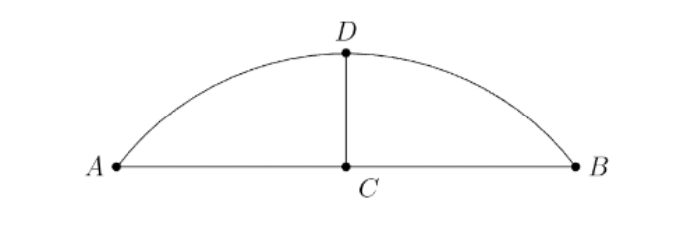
\includegraphics[width=\columnwidth]{olympiad/figs/permo.jpg}
			\caption{}
			\label{fig:plate}
    \end{figure}



    $ C $ is the midpoint of $ AB $, and $ D $ is the midpoint of arc $ AB $. Given that $ AB = 24 $ cm and $ CD = 6 $ cm, what is the radius of the plate in centimeters? (The figure is not drawn to scale.)\hfill(PRMO 2015)
    \item In the coordinate plane, a point is called a lattice point if both of its coordinates are integers. Let $A$ be the point $\brak{12, 84}$. Find the number of right-angled triangles $ABC$ in the coordinate plane where $B$ and $C$ are lattice points, having a right angle at the vertex $A$ and whose incenter is at the origin $\brak{0, 0}$.\hfill(IOQM 2015)
\item Let $ABC$ be an acute-angled triangle with orthocentre $H$, and let $W$ be a point on the side $BC$, lying strictly between $B$ and $C$. The points $M$ and $N$ are the feet of the altitudes from $B$ and $C$ respectively. Denote by $\omega_1$ the circumcircle of $BWN$, and let $X$ be the point on $\omega_1$ such that $WX$ is a diameter of $\omega_1$. Analogously, denote by $\omega_2$ the circumcircle of $CWM$ and let $Y$ be the point on $\omega_2$ such that $WY$ is a diameter of $\omega_2$. Prove that $X$, $Y$ and $H$ are collinear. \hfill(IMO  2013)
\item Let $ABC$ be an acute-angled triangle with circumcentre $O$. Let $P$ on $BC$ be the foot of the altitude from $A$. Suppose that $\angle BC A\geq \angle ABC+30\degree$. Prove that $\angle CAB+\angle COP < \angle 90\degree$.\hfill(IMO 2001)
\item Let $R$ and $S$ be different points on a circle $\Omega$ such that $RS$ is not a diameter. Let $l$ be the tangent line to $\Omega$ at $R$. Point $T$ is such that $S$ is the midpoint of the line segment $RT$. Point $J$ is chosen on the shorter arc $RS$ of $\Omega$ so that the circumcircle $\Gamma$ of triangle $JST$ intersects $l$ at two distinct points. Let $A$ be the common point of $\Gamma$ and $l$ that is closer to $R$. Line $AJ$ meets $\Omega$ again at $K$. Prove that the line $KT$ is tangent to $\Gamma$.\hfill (IMO  2017)
\end{enumerate}

%
\section{Identities}
\subsection{NCERT}
 Verify
\begin{enumerate}[label=\thesubsection.\arabic*.,ref=\thesubsection.\theenumi,resume*]
	\item $x^3+y^3 = \brak{x+y}\brak{x^2-xy+y^2}$
	\item $x^3-y^3 = \brak{x-y}\brak{x^2+xy+y^2}$
	\item $x^3+y^3+z^3-3xyz = \frac{1}{2}\brak{x+y+z}\sbrak{\brak{x-y}^{2}+\brak{y-z}^{2}+\brak{z-x}^{2}}$
\end{enumerate}
Factorize each of the following
\begin{enumerate}[label=\thesubsection.\arabic*.,ref=\thesubsection.\theenumi]
	\item $8a^3+b^3+12a^2b+6ab^2$
	\item $8a^3-b^3-12a^2b+6ab^2$
	\item $27-125a^3-135a+225a^2$
	\item $64a^3-27b^3-144a^2b+108ab^2$
	\item $27p^3-\frac{1}{216}-\frac{9}{2}p^2 + \frac{p}{4}$
	\item $27y^3+125z^3$ 
	\item $64m^3-343n^3$
	\item $27x^3+y^3+z^3-9xyz$
\end{enumerate}
Find the value of each of the following 
\begin{enumerate}[label=\thesubsection.\arabic*.,ref=\thesubsection.\theenumi,resume*]
	\item $\brak{-12}^3+\brak{7}^3+\brak{5}^3$
	\item $\brak{28}^3+\brak{-15}^3+\brak{-13}^3$
\end{enumerate}
Give possible expressions for the length and breadth of each of the following rectangles, in which their areas are given
\begin{enumerate}[label=\thesubsection.\arabic*.,ref=\thesubsection.\theenumi,resume*]
	\item $25a^2-35a+12$
	\item $35a^2+13y-12$
\end{enumerate}
What are the possible expressions for the dimensions of the cuboids whose volumes are given below
\begin{enumerate}[label=\thesubsection.\arabic*.,ref=\thesubsection.\theenumi,resume*]
	\item $3x^2-12x$
	\item $12ky^2+8ky-20k$
\end{enumerate}

\subsection{CBSE}
 Verify
\begin{enumerate}[label=\thesubsection.\arabic*.,ref=\thesubsection.\theenumi,resume*]
	\item $x^3+y^3 = \brak{x+y}\brak{x^2-xy+y^2}$
	\item $x^3-y^3 = \brak{x-y}\brak{x^2+xy+y^2}$
	\item $x^3+y^3+z^3-3xyz = \frac{1}{2}\brak{x+y+z}\sbrak{\brak{x-y}^{2}+\brak{y-z}^{2}+\brak{z-x}^{2}}$
\end{enumerate}
Factorize each of the following
\begin{enumerate}[label=\thesubsection.\arabic*.,ref=\thesubsection.\theenumi]
	\item $8a^3+b^3+12a^2b+6ab^2$
	\item $8a^3-b^3-12a^2b+6ab^2$
	\item $27-125a^3-135a+225a^2$
	\item $64a^3-27b^3-144a^2b+108ab^2$
	\item $27p^3-\frac{1}{216}-\frac{9}{2}p^2 + \frac{p}{4}$
	\item $27y^3+125z^3$ 
	\item $64m^3-343n^3$
	\item $27x^3+y^3+z^3-9xyz$
\end{enumerate}
Find the value of each of the following 
\begin{enumerate}[label=\thesubsection.\arabic*.,ref=\thesubsection.\theenumi,resume*]
	\item $\brak{-12}^3+\brak{7}^3+\brak{5}^3$
	\item $\brak{28}^3+\brak{-15}^3+\brak{-13}^3$
\end{enumerate}
Give possible expressions for the length and breadth of each of the following rectangles, in which their areas are given
\begin{enumerate}[label=\thesubsection.\arabic*.,ref=\thesubsection.\theenumi,resume*]
	\item $25a^2-35a+12$
	\item $35a^2+13y-12$
\end{enumerate}
What are the possible expressions for the dimensions of the cuboids whose volumes are given below
\begin{enumerate}[label=\thesubsection.\arabic*.,ref=\thesubsection.\theenumi,resume*]
	\item $3x^2-12x$
	\item $12ky^2+8ky-20k$
\end{enumerate}

\subsection{JEE}
 Verify
\begin{enumerate}[label=\thesubsection.\arabic*.,ref=\thesubsection.\theenumi,resume*]
	\item $x^3+y^3 = \brak{x+y}\brak{x^2-xy+y^2}$
	\item $x^3-y^3 = \brak{x-y}\brak{x^2+xy+y^2}$
	\item $x^3+y^3+z^3-3xyz = \frac{1}{2}\brak{x+y+z}\sbrak{\brak{x-y}^{2}+\brak{y-z}^{2}+\brak{z-x}^{2}}$
\end{enumerate}
Factorize each of the following
\begin{enumerate}[label=\thesubsection.\arabic*.,ref=\thesubsection.\theenumi]
	\item $8a^3+b^3+12a^2b+6ab^2$
	\item $8a^3-b^3-12a^2b+6ab^2$
	\item $27-125a^3-135a+225a^2$
	\item $64a^3-27b^3-144a^2b+108ab^2$
	\item $27p^3-\frac{1}{216}-\frac{9}{2}p^2 + \frac{p}{4}$
	\item $27y^3+125z^3$ 
	\item $64m^3-343n^3$
	\item $27x^3+y^3+z^3-9xyz$
\end{enumerate}
Find the value of each of the following 
\begin{enumerate}[label=\thesubsection.\arabic*.,ref=\thesubsection.\theenumi,resume*]
	\item $\brak{-12}^3+\brak{7}^3+\brak{5}^3$
	\item $\brak{28}^3+\brak{-15}^3+\brak{-13}^3$
\end{enumerate}
Give possible expressions for the length and breadth of each of the following rectangles, in which their areas are given
\begin{enumerate}[label=\thesubsection.\arabic*.,ref=\thesubsection.\theenumi,resume*]
	\item $25a^2-35a+12$
	\item $35a^2+13y-12$
\end{enumerate}
What are the possible expressions for the dimensions of the cuboids whose volumes are given below
\begin{enumerate}[label=\thesubsection.\arabic*.,ref=\thesubsection.\theenumi,resume*]
	\item $3x^2-12x$
	\item $12ky^2+8ky-20k$
\end{enumerate}

\section{Equations}
\subsection{NCERT}
 \input{ncert/eq.tex}
\subsection{CBSE}
 \input{cbse/eq.tex}
\subsection{JEE}
 \input{JEE/eq.tex}
 %\input{JEE/zchapters/trigonometric-functions-equations.tex}
\section{Inequalities}
\subsection{NCERT}
\input{./chapters/trig/ineq}
\subsection{JEE}
\input{JEE/ineq}
%\appendices
\fi
\end{document}

